\documentclass{article}

% 在主文件的 \documentclass 之后加载；建议使用 XeLaTeX 编译。
% 此文件集中加载宏包，具体版式与自定义命令分别放在 layout-portrait.tex 和 mystyle.tex 中。

% 中文支持；不采用 ctex 的中文标题名称与版式方案。
% 无布局的独立接口测试使用 Fandol；正式字体由 layout-portrait.tex 覆盖。
\PassOptionsToPackage{fontset=fandol}{ctex}
\usepackage[scheme=plain]{ctex}

% 数学公式、矩阵、对齐环境与数学符号（含 \mathbb）。
\usepackage{amsmath}
\usepackage{amssymb}
\usepackage{unicode-math}

% 图片与颜色。
\usepackage{graphicx}
\usepackage{xcolor}

% 删除线；normalem 保留 \emph 的原有强调语义。
\usepackage[normalem]{ulem}

% 页面尺寸、边距与多栏排版；具体参数在 layout-portrait.tex 中设置。
\usepackage{geometry}
\usepackage{multicol}
\usepackage{titlesec}
\usepackage{needspace}
\usepackage{enumitem}
\usepackage{fancyhdr}
\usepackage{tocloft}
\usepackage{lastpage}
\usepackage{etoolbox}
\usepackage{newunicodechar}

% 代码高亮，以及后续代码标题栏、引用块所需的盒子支持。
\usepackage{minted}
\usepackage{tcolorbox}
\tcbuselibrary{skins,breakable,minted}

% 目录链接、URL 和交叉引用；在上述宏包之后加载。
\usepackage[
    hidelinks
]{hyperref}

% 横版布局：只放本版参数；三版共用的实现及双栏机制见 preamble/shared/。
% A4 横向双栏；四边 12 mm，上下包含页眉、页脚及其间距。
\geometry{
  a4paper,landscape,left=12mm,right=12mm,top=12mm,bottom=12mm,
  includeheadfoot,headheight=12pt,headsep=4mm,footskip=6mm
}

% 正文、数学、行内等宽与代码块字体及单色符号见共用文件。
% 三版共用的字体：正文与导航、单色符号、数学、行内等宽与代码块。
% 由各版布局在 \geometry 之后 \input；字号、行距等参数由各版布局设置。
% 本机字体须可供 XeLaTeX 访问，不静默替换。

% 正文与导航字体：使用与已确认样张一致的 Latin Modern Roman 10 pt 静态字形。
\setmainfont{lmroman10}[
  Extension=.otf,UprightFont=*-regular,BoldFont=*-bold,
  ItalicFont=*-italic,BoldItalicFont=*-bolditalic
]
\setsansfont{PingFang SC}[BoldFont={PingFang SC Semibold}]
\setCJKmainfont{Songti SC}[BoldFont={Songti SC Bold},ItalicFont={Songti SC}]
\setCJKsansfont{PingFang SC}[BoldFont={PingFang SC Semibold}]
% 宋体正文的双引号改用当前西文正文字形（用户确认），输入仍为 Unicode “”。
% 跟随 NFSS 字体族选择：粗体/斜体保留规则，苹方与 Maple（含自定义代码字体）恢复原分类。
% 保存 xeCJK 已分配的类号，不硬编码；半角左右标点类取自西文圆括号。
% 不在 selectfont 中反复调用 xeCJKDeclareCharClass：它会全局追加字符范围表。
% 这里只作局部 XeTeXcharclass 赋值，嵌套字体分组结束时自然恢复外层分类。
\makeatletter
\chardef\BookQuoteFullLeft=\XeTeXcharclass"201C
\chardef\BookQuoteFullRight=\XeTeXcharclass"201D
\chardef\BookQuoteHalfLeft=\XeTeXcharclass`\(
\chardef\BookQuoteHalfRight=\XeTeXcharclass`\)
\newcommand{\BookSelectQuoteClass}{%
  \ifx\f@family\rmdefault
    \XeTeXcharclass"201C=\BookQuoteHalfLeft
    \XeTeXcharclass"201D=\BookQuoteHalfRight
  \else
    \XeTeXcharclass"201C=\BookQuoteFullLeft
    \XeTeXcharclass"201D=\BookQuoteFullRight
  \fi}
\AddToHook{selectfont}[book/quotes]{\BookSelectQuoteClass}
\makeatother
% 单色符号使用项目内的静态字体；标题中也保持常规直立字重。
% 只映射原稿实际使用的两个字符，不更改正文或全局字符分类。
\newfontfamily\BookSymbolFont{NotoEmoji-Regular.ttf}[
  Path=preamble/fonts/,
  BoldFont=NotoEmoji-Regular.ttf,
  ItalicFont=NotoEmoji-Regular.ttf,
  BoldItalicFont=NotoEmoji-Regular.ttf
]
% xeCJK 默认借用当前字体空格；Noto Emoji 的空格宽达 1.27em。
% 仅在符号局部分组内固定中西文间距，避免中文后的符号被推远。
\DeclareRobustCommand{\BookStar}{{%
  \xeCJKsetup{CJKecglue={\hskip .25em\relax}}%
  \BookSymbolFont\char"2B50\relax}}
\DeclareRobustCommand{\BookFlag}{{%
  \xeCJKsetup{CJKecglue={\hskip .25em\relax}}%
  \BookSymbolFont\char"1F6A9\relax}}
\newunicodechar{⭐}{\BookStar}
\newunicodechar{🚩}{\BookFlag}
% 书签保留原 Unicode，避免把字体命令写入 PDF 字符串。
\pdfstringdefDisableCommands{%
  \def⭐{\string⭐}%
  \def🚩{\string🚩}%
}
\setmathfont{Latin Modern Math}
% 直立数学字母与算子均使用数学字体；\text 仍使用正文字体。
% 显式外层分组兼容原稿的 ^\mathrm{mid}、_\mathrm{mid} 写法。
% 直接使用 mathrm=sym 时，unicode-math 的内部组命令不能充当上下标组。
% 在 unicode-math 完成文档起始初始化后设置，避免被其默认定义覆盖。
\AddToHook{begindocument/end}{\renewcommand{\mathrm}[1]{{\symup{#1}}}}
\setoperatorfont{\symup}
% 保留 \boldsymbol 对完整表达式（含算子和定界符）的语义。
% 数学字体没有独立粗体文件，bold 版本采用轻度合成加粗。
\setmathfont{Latin Modern Math}[version=bold,FakeBold=1.2]
% 保留文本类数学字母（如 \mathbf、\mathit）的 bold 版本字体映射。
% \mathrm 已由上方定义改用数学字形，不走此文本映射。
\setboldmathrm{lmroman10}[
  Extension=.otf,UprightFont=*-bold,BoldFont=*-bold,
  ItalicFont=*-bolditalic,BoldItalicFont=*-bolditalic
]

% 行内等宽文字使用 Maple，字号随所在正文；与代码块采用相同字形特性。
\setmonofont{Maple Mono NF CN}[
  Ligatures={NoCommon,NoContextual,NoDiscretionary,NoHistoric},
  RawFeature={-calt;-tlig;+cv01;+cv32;+cv33;+cv34;+cv35;+cv36;+cv37}
]
\setCJKmonofont{Maple Mono NF CN}[
  Ligatures={NoCommon,NoContextual,NoDiscretionary,NoHistoric},
  RawFeature={-calt;-tlig;+cv01;+cv32;+cv33;+cv34;+cv35;+cv36;+cv37}
]

% 只供 minted 使用（fontfamily=bookcode）；不改变 \texttt 或代码标题栏。
% 禁用标准、上下文、可选、历史连字，以及 calt/TeX 字符替换。
% cv01 去除符号间隙；cv32--cv37 将手写斜体改为常规斜体（仍保留倾斜）。
\newfontfamily\BookCodeLatin{Maple Mono NF CN}[
  Ligatures={NoCommon,NoContextual,NoDiscretionary,NoHistoric},
  RawFeature={-calt;-tlig;+cv01;+cv32;+cv33;+cv34;+cv35;+cv36;+cv37}
]
\newCJKfontfamily\BookCodeCJK{Maple Mono NF CN}[
  Ligatures={NoCommon,NoContextual,NoDiscretionary,NoHistoric},
  RawFeature={-calt;-tlig;+cv01;+cv32;+cv33;+cv34;+cv35;+cv36;+cv37}
]
\makeatletter
\@namedef{FV@fontfamily@bookcode}{%
  \def\FV@FontScanPrep{}%
  \def\FV@FontFamily{\BookCodeLatin\BookCodeCJK}%
}
\makeatother

% 页眉页脚、目录点线与代码配色见共用文件。
% 三版共用的配色，由各版布局在 shared/fonts.tex 之后 \input。
% 页眉页脚、目录、代码样式与扉页引用这里的颜色；mystyle.tex 中各接口自带的颜色不在此处。

% 页眉、页脚与次要文字。
\definecolor{BookMuted}{HTML}{666666}
% 目录二、三级条目的点线。
\definecolor{BookTOCDots}{HTML}{888888}
% 代码阅读 / 打印配色：仅两种彩色；名称、调用与标点保持深灰。
\definecolor{BookCodeText}{HTML}{30343B}
\definecolor{BookCodeBlue}{HTML}{506B82}
\definecolor{BookCodeGreen}{HTML}{58715D}
\definecolor{BookCodeComment}{HTML}{70757D}
% 扉页：主要文字、次要文字与细框；唯一强调色与代码高亮的蓝灰一致。
\definecolor{BookTitlePageInk}{HTML}{1D1D1F}
\definecolor{BookTitlePageSecondary}{HTML}{6E6E73}
\definecolor{BookTitlePageHairline}{HTML}{D1D1D6}
\colorlet{BookTitlePageAccent}{BookCodeBlue}

\makeatletter
% 固定正文及常用相对字号，数学上下间距随正常字号一起恢复。
\renewcommand\normalsize{%
  \@setfontsize\normalsize{10pt}{14pt}%
  \abovedisplayskip=7pt plus 2pt minus 2pt
  \belowdisplayskip=7pt plus 2pt minus 2pt
  \abovedisplayshortskip=3pt plus 1pt
  \belowdisplayshortskip=5pt plus 1pt minus 1pt
}
\renewcommand\small{\@setfontsize\small{9pt}{12pt}}
\renewcommand\footnotesize{\@setfontsize\footnotesize{8pt}{10.5pt}}
\makeatother
\normalsize
\setlength{\parindent}{0pt}
\setlength{\parskip}{2pt plus 1pt minus 1pt}
% 窄栏含较长行内公式时，增加断行算法的应急伸展量；不改变正常行距。
% 用户确认 6em（曾试改 3em 后撤回）：3em 时 Overfull 较多，6em 只留少量过松行。
\setlength{\emergencystretch}{6em}
\raggedbottom
\clubpenalty=10000
\widowpenalty=10000
\displaywidowpenalty=10000
\setlist{topsep=3pt,itemsep=1pt,parsep=1pt,partopsep=0pt,leftmargin=*}
% 二级无序列表用空心圆点（用户确认）；Latin Modern 的 U+25E6 与一级圆点外框相同，只差填充。
\renewcommand{\labelitemii}{\labelitemfont\textopenbullet}

\titleformat{\section}{\sffamily\bfseries\fontsize{16}{21}\selectfont}{}{0pt}{\BookChapterAnchor}
\titleformat{\subsection}{\sffamily\bfseries\fontsize{12}{17}\selectfont}{}{0pt}{}
\titleformat{\subsubsection}{\sffamily\bfseries\fontsize{10.5}{15}\selectfont}{}{0pt}{}
\titlespacing*{\section}{0pt}{10pt}{5pt}
\titlespacing*{\subsection}{0pt}{8pt plus 2pt minus 2pt}{4pt}
\titlespacing*{\subsubsection}{0pt}{6pt plus 2pt minus 1pt}{3pt}
\titleformat{\paragraph}{\sffamily\bfseries\fontsize{10}{14}\selectfont}{}{0pt}{}
\titleformat{\subparagraph}{\sffamily\bfseries\fontsize{10}{14}\selectfont}{}{0pt}{}
\titlespacing*{\paragraph}{0pt}{5pt}{2pt}
\titlespacing*{\subparagraph}{0pt}{4pt}{2pt}
% 栏距；启动双栏、通栏目录标题、页顶所在章的页眉与图片按栏宽见 shared/twocolumn.tex。
\setlength{\columnsep}{8mm}

% 标题编号、目录条目与书签设置，以及双栏机制见共用文件。
% 三版共用的标题编号、目录条目与书签设置，由各版布局在设置字号之后 \input。
% 目录标题及目录前后的分页由各版负责：竖版用 tocloft 的标题设置，双栏版本见 shared/twocolumn.tex。
% 每次排目录前须把 \BookTOCPreviousLevel 清零：竖版在布局中挂钩，双栏版本在重定义的 \tableofcontents 中清零。

% 保留原文的 0xPQ 编号：只关闭章节标题的自动编号。
\setcounter{secnumdepth}{-1}
% 目录展开到三级；PDF 书签包含全部标题层级并默认全部展开。
\setcounter{tocdepth}{3}
\hypersetup{bookmarksdepth=5,bookmarksopen=true}
\renewcommand{\contentsname}{目录}
% 方案 A：一级沿用苹方 Semibold；二三级沿用正文宋体与 Latin Modern Roman。
\newlength{\BookTOCUnit}
\settowidth{\BookTOCUnit}{\normalfont\fontsize{10}{15}\selectfont 中}
% 每条目录装入完整段落盒：续行保持本级缩进，页码固定在末行右端。
% 条目间使用可丢弃的竖直间距，页首不残留标题前留白。
% 根据前后层级禁止父标题与首个子条目之间分页，不捆绑整个章节。
\makeatletter
\newcount\BookTOCPreviousLevel
\BookTOCPreviousLevel=0
\newcommand{\BookTOCEntry}[4]{%
  \par
  \ifnum\BookTOCPreviousLevel=1 \penalty10000
  \else\ifnum\BookTOCPreviousLevel=2
    \ifnum#1=3 \penalty10000\else\penalty0\fi
  \else\penalty0\fi\fi
  \begingroup
  \@tempdima=0pt
  \ifnum\BookTOCPreviousLevel=1 \advance\@tempdima by5pt\fi
  \ifnum#1=1 \advance\@tempdima by12pt\fi
  \vskip\@tempdima
  \nointerlineskip
  \vbox{%
    \hsize=\linewidth
    \normalfont\fontsize{10}{15}\selectfont
    \ifnum#1=1 \sffamily\bfseries\fontsize{12}{15}\selectfont
    \else\ifnum#1=2 \fontsize{10.5}{15}\selectfont\fi\fi
    \leftskip=#2\relax \rightskip=30pt
    \parfillskip=-\rightskip \parindent=0pt \parskip=0pt
    \interlinepenalty=10000
    \noindent\strut#3\nobreak
    \ifnum#1=1 \hfill
    % 9pt 是实际点中心间距；两端各留 3pt，空间不足一格时不绘点。
    \else{\normalfont\fontsize{10}{15}\selectfont\color{BookTOCDots}%
      \kern3pt\leaders\hbox to9pt{\hss.\hss}\hfill\kern3pt}\fi
    \nobreak\hb@xt@20pt{\hfil\normalfont
      \ifnum#1=1 \fontsize{11}{15}\else\fontsize{10}{15}\fi\selectfont#4}\strut\par
  }%
  \endgroup
  \global\BookTOCPreviousLevel=#1\relax}
\renewcommand*{\l@section}[2]{%
  \ifnum\c@tocdepth>0 \BookTOCEntry{1}{0pt}{#1}{#2}\fi}
\renewcommand*{\l@subsection}[2]{%
  \ifnum\c@tocdepth>1 \BookTOCEntry{2}{2\BookTOCUnit}{#1}{#2}\fi}
\renewcommand*{\l@subsubsection}[2]{%
  \ifnum\c@tocdepth>2 \BookTOCEntry{3}{4\BookTOCUnit}{#1}{#2}\fi}
\makeatother

% 横版与代码版共用的双栏机制：启动双栏、通栏目录标题、页顶所在章的页眉、图片按栏宽解释 \textwidth。
% 由两版布局在 shared/toc.tex 之后 \input；栏距等版面参数由各版布局设置，
% 一级标题格式须在标题文字处调用 \BookChapterAnchor。

% 入口无排版选项；启动标准双栏输出，章节自然连续，不平衡章末。
\setlength{\columnseprule}{0pt}
\AddToHook{begindocument/end}{\twocolumn\raggedbottom}

% 目录标题由下方重写的 \tableofcontents 以通栏居中排出（22/28 pt，后接 16pt），
% 不使用 tocloft 的标题设置。
\makeatletter
% tocloft 在 begindocument 中重定义入口，此处在其初始化结束后安装。
% 标准双栏的可选通栏头只用于目录首张；条目仍按栏自然流动。
\AddToHook{begindocument/end}{%
  \renewcommand{\tableofcontents}{%
    \clearpage
    \markboth{}{}%
    \global\BookTOCPreviousLevel=0
    \twocolumn[{%
      \centering\sffamily\bfseries\fontsize{22}{28}\selectfont
      \contentsname\par\vspace{16pt}%
    }]%
    \@starttoc{toc}%
    \clearpage
  }%
}
\makeatother

% 页眉显示页顶所在的一级标题（用户确认，2026-10-14）：
% 本页没有新章，或新章不在左栏顶端时，取页首延续的章（TopMark）；
% 本页第一个新章恰好位于左栏顶端时，取该章。章节连续排版，
% 一页可含多章，不能沿用竖版取本页最后标记的 \leftmark。
% 位置由标题文字内的 \pdfsavepos 记录，需两轮编译；run.sh 至少两轮。
\makeatletter
\NewMarkClass{book-chapter}
\newcounter{BookChapter}
\AddToHook{cmd/section/before}{\stepcounter{BookChapter}}
% 置于标题文字内部，保证位置与标题同在一栏，不会因断页与标题分离。
\newcommand{\BookChapterAnchor}[1]{%
  \leavevmode\pdfsavepos
  \RecordProperties{BookChapter@\the\value{BookChapter}}{xpos,ypos}#1}
\newdimen\BookChapterTopLimit
\newcommand{\BookHeaderChapter}{%
  \begingroup
  \edef\BookTop{\TopMark{book-chapter}}%
  \edef\BookFirst{\FirstMark{book-chapter}}%
  \let\BookShown\BookTop
  \ifx\BookTop\BookFirst\else
    \ifx\BookTop\@empty\let\BookShown\BookFirst\fi
    % 左栏顶端标题的基线距版心顶约一个 topskip；留 20pt 容差，
    % 上方哪怕只有一行正文，标题基线也会再低约 30pt。
    \BookChapterTopLimit=\dimexpr\paperheight-1in-\voffset-\topmargin
      -\headheight-\headsep-\topskip-20pt\relax
    \ifdim\RefProperty{BookChapter@\BookFirst}{xpos}sp<.5\paperwidth
      \ifdim\RefProperty{BookChapter@\BookFirst}{ypos}sp>\BookChapterTopLimit
        \let\BookShown\BookFirst
      \fi
    \fi
  \fi
  \ifx\BookShown\@empty\else
    \csname BookChapterName@\BookShown\endcsname
  \fi
  \endgroup}
\makeatother
\pagestyle{fancy}
\fancyhf{}
\fancyhead[L]{\sffamily\fontsize{8}{10}\selectfont\color{BookMuted}%
  \BookHeaderChapter}
\fancyfoot[C]{\sffamily\fontsize{8}{10}\selectfont\color{BookMuted}\thepage}
\renewcommand{\headrulewidth}{0pt}
\renewcommand{\footrulewidth}{0pt}
% 保留标准标记，另记章号及章名供页眉判断页顶所在的章。
\renewcommand{\sectionmark}[1]{%
  \markboth{#1}{}%
  \expandafter\gdef\csname BookChapterName@\the\value{BookChapter}\endcsname{#1}%
  \InsertMark{book-chapter}{\the\value{BookChapter}}}
\renewcommand{\subsectionmark}[1]{\markright{#1}}
\fancypagestyle{plain}{\fancyhf{}\fancyfoot[C]{\sffamily\fontsize{8}{10}\selectfont\color{BookMuted}\thepage}}

% 双栏图片按当前容器计算正文宽度；保持原路径、可选参数和长宽比。
% 用户已批准将现有 0.8\textwidth / \textwidth 分别解释为 0.8 / 1 栏宽。
% 局部分组避免改变双栏输出的整页 textwidth。
\NewCommandCopy{\BookIncludeGraphics}{\includegraphics}
\RenewDocumentCommand{\includegraphics}{s O{} m}{%
  \begingroup
  \setlength{\textwidth}{\linewidth}%
  \IfBooleanTF{#1}
    {\BookIncludeGraphics*[#2]{#3}}
    {\BookIncludeGraphics[#2]{#3}}%
  \endgroup
}


% 代码块的词法配色、minted 默认设置与代码卡片标题见共用文件。
% 三版共用的代码块样式：Pygments 词法配色、minted 默认设置与代码卡片标题。
% 由各版布局在 shared/fonts.tex、shared/colors.tex 之后 \input。
% 某版需要不同的代码字号时，在 \input 之后用 \setminted{fontsize=…} 覆盖。

% 使用 bw 提供 Pygments 转义与分词接口，在每次加载样式后替换 token 外观。
% 兼容目标：minted 3.x / Pygments 2.x；不安装系统 Python 插件。
% 未列出的 token 不增加颜色、粗体、下划线或错误边框。
\makeatletter
\newcommand{\BookCodeBlueText}[1]{\textcolor{BookCodeBlue}{#1}}
\newcommand{\BookCodeGreenText}[1]{\textcolor{BookCodeGreen}{#1}}
\newcommand{\BookCodeCommentText}[1]{\textcolor{BookCodeComment}{#1}}
\def\BookToken@k{\let\PYG@tc\BookCodeBlueText}
\let\BookToken@m\BookToken@k
\let\BookToken@no\BookToken@k
\let\BookToken@ow\BookToken@k
% 内建名称：C++ 的 true、false、NULL，Bash、Python 的内建命令与函数。
\let\BookToken@nb\BookToken@k
\def\BookToken@s{\let\PYG@tc\BookCodeGreenText}
\def\BookToken@c{\let\PYG@tc\BookCodeCommentText}
\def\BookToken@cp{\let\PYG@tc\BookCodeBlueText\let\PYG@it\relax}
\def\BookToken@cpf{\let\PYG@tc\BookCodeGreenText\let\PYG@it\relax}
% Pygments 2.19、2.20 把 1ll、1llu、1lu 分成浮点数 1l 与名称 l、lu、u（pygments/pygments#1847），
% 把 C++23 的 1z、1uz、1zu 分成整数与名称 z、zu。数字后紧跟只由 l、u、z（含大写）组成的名称时，
% 名称只会是拆开的后缀，改按数字着色；10_km 等自定义后缀以下划线开头，不受影响。上游修复进入 TeX Live 后可删除。
% fvextra 给每个 token 加分组，折行时又以 \FancyVerbBreakStart/Stop 包住内容，故用全局状态，匹配时容许这层包装。
% 每行先测宽再排版，每遍都从 \FancyVerbFormatText 开始，在此清除上一遍留下的状态。
\ExplSyntaxOn
\bool_new:N \g__book_code_after_number_bool
\regex_const:Nn \c__book_code_suffix_regex
  { \A (?: \c{FancyVerbBreakStart} )? [lLuUzZ]{1,3} (?: \c{FancyVerbBreakStop} )? \Z }
\cs_new_protected:Npn \BookCode@Suffix #1#2
  {
    \bool_if:NT \g__book_code_after_number_bool
      {
        \str_if_eq:nnT {#1} {n}
          { \regex_match:NnT \c__book_code_suffix_regex {#2} { \BookToken@m } }
      }
    \str_if_eq:eeTF { \str_range:nnn {#1} { 1 } { 3 } } { l+m }
      { \bool_gset_true:N \g__book_code_after_number_bool }
      { \bool_gset_false:N \g__book_code_after_number_bool }
  }
\cs_new_eq:NN \__book_code_format_text:n \FancyVerbFormatText
\cs_set_protected:Npn \FancyVerbFormatText #1
  {
    \bool_gset_false:N \g__book_code_after_number_bool
    \__book_code_format_text:n {#1}
  }
\ExplSyntaxOff
% Pygments 的 Bash 词法把 <0.in、diff 1.out 中文件名开头的数字单独标为数字（Literal.Number），
% 其后的 .in、.out 是不经 \PYG 的普通文字；数字后紧跟“.”时改按普通文字排。
% fvextra 在每个 token 之后结束分组，故越过这个 \endgroup 再看下一个字符；不是 \endgroup 时照常着色。
\def\BookCode@Number#1{\@ifnextchar\endgroup{\BookCode@Number@i{#1}}{\PYG@do{#1}}}
\def\BookCode@Number@i#1\endgroup{%
  \@ifnextchar.{\let\PYG@tc\relax\PYG@do{#1}\endgroup}{\PYG@do{#1}\endgroup}}
\AddToHook{cmd/minted@defstyle/after}{%
  \edef\BookCodeStyle{\mintedtexoptvalueof{style}}%
  \ifdefstring{\BookCodeStyle}{bw}{%
    \def\PYG@tok#1{\ifcsname BookToken@#1\endcsname
      \csname BookToken@#1\endcsname\fi}%
    % 同 Pygments 的 \PYG，只加入上面两项处理。
    \def\PYG#1#2{\PYG@reset\PYG@toks#1+\relax+\BookCode@Suffix{#1}{#2}%
      \ifstrequal{#1}{l+m}{\BookCode@Number{#2}}{\PYG@do{#2}}}%
  }{}%
}
\makeatother
\setminted{
  fontfamily=bookcode,fontsize=\fontsize{8}{10.5}\selectfont,
  baselinestretch=1,style=bw,linenos=false,
  formatcom=\color{BookCodeText}\mdseries\upshape,
  breaklines=true,breakanywhere=false,tabsize=4
}
% 词法高亮并非 C++ 语义分析；仅补充明确要求的三个标准库类型名称、本书的整数类型别名 i64、i128、u64、u32，
% 以及 GCC 的 __int128_t、__uint128_t（__int128 已是关键字）。这些别名与 GCC 类型名不会用作变量名。
\setminted[cpp]{extrakeywordstype={vector,string,pair,i64,i128,u64,u32,__int128_t,__uint128_t}}
\setminted[c++]{extrakeywordstype={vector,string,pair,i64,i128,u64,u32,__int128_t,__uint128_t}}
\setminted[cxx]{extrakeywordstype={vector,string,pair,i64,i128,u64,u32,__int128_t,__uint128_t}}
\newfontfamily\BookCodeTitleLatin{PingFang SC Medium}
\newCJKfontfamily\BookCodeTitleCJK{PingFang SC Medium}
% coltext 同时保证 tcolorbox 续页恢复深灰，而非默认纯黑。
\tcbset{input-code-title/.style={coltext=BookCodeText,fonttitle=\mdseries\upshape\BookCodeTitleLatin\BookCodeTitleCJK\fontsize{9}{12}\selectfont}}
% 代码卡片与引用块共用的前后距，取代 tcolorbox 默认的 beforeafter skip balanced；
% 长度 \BookBoxBeforeSkip、\BookBoxAfterSkip 由各版布局设定。
% 盒前用 tcolorbox 的 before skip：盒顶距上一行的底为前距，盒与盒之间也是这个距离。
% 紧跟标题时 tcolorbox 不执行盒前设置（\iftcb@nobreak），标题与盒之间不受影响。
% 盒后把 \prevdepth 归零再加后距：后接正文时按段距与行距接排，后接标题时盒底相当于上一行的基线。
\makeatletter
\tcbset{book-box-spacing/.style={
  before skip=\BookBoxBeforeSkip,
  after={\tcb@parfillskip@check\par\ifvmode\prevdepth\z@\addvspace{\BookBoxAfterSkip}\fi}}}
\makeatother


% 扉页：外观与提交信息读取见共用文件；入口提供书名、作者、英文书名与配图路径。
% 版面沿用竖版的元素与间距，按 A4 横向重排：书名基线距页顶 48 mm，提交信息底边距纸边 17 mm；
% 页高只有 210 mm，配图区由竖版的 130 × 110 mm 收紧为 110 × 70 mm。
% 三版共用的扉页：书名、英文书名、作者、配图，以及底部的仓库地址与 Last commit；设了版本标记时悬挂在书名右侧。
% 由各版布局在 shared/fonts.tex、shared/colors.tex 之后 \input，再用 \TitlePageSetup 给出本版的版面参数。
% 书名、作者、英文书名、配图路径、版本标记与仓库地址由入口提供；路径均相对于项目根目录。
% 绝对定位依赖 TikZ 的 remember picture，至少编译两轮（根目录 run.sh 已保证）。

\newfontfamily\BookTitlePageMediumLatin{PingFang SC Medium}
\newCJKfontfamily\BookTitlePageMediumCJK{PingFang SC Medium}
% 提交信息的眉题：小号大写，加宽字距。
\newfontfamily\BookTitlePageEyebrow{PingFang SC Medium}[LetterSpace=14]
% 提交说明原样输出：此字体族不启用 TeX 连字，-- 等不会被替换。
\newfontfamily\BookTitlePagePlainLatin{PingFang SC}

% 版面参数：以纸张中心为原点，书名、英文书名、作者的基线，配图区中心，底部信息区底边的纵向位置，
% 以及配图区的宽和高。配图在配图区内等比缩放后居中；标题区与底部信息区的位置不随图片比例变化。
% 各版布局须给出全部 7 项，缺少时编译报错；数值按原文交给 TikZ 与 \setlength，不预先换算。
\newlength{\BookTitlePageImageWidth}
\newlength{\BookTitlePageImageHeight}
\pgfkeys{
  /book/titlepage/.is family,
  /book/titlepage/title/.store in=\BookTitlePageTitleY,
  /book/titlepage/english/.store in=\BookTitlePageEnglishY,
  /book/titlepage/author/.store in=\BookTitlePageAuthorY,
  /book/titlepage/image/.store in=\BookTitlePageImageY,
  /book/titlepage/stamp/.store in=\BookTitlePageStampY,
  /book/titlepage/image-width/.code={\setlength{\BookTitlePageImageWidth}{#1}},
  /book/titlepage/image-height/.code={\setlength{\BookTitlePageImageHeight}{#1}},
}
\newcommand{\TitlePageSetup}[1]{\pgfkeys{/book/titlepage/.cd,#1}}

\makeatletter
% 元信息：英文书名、配图路径与版本标记；不写或参数为空时省略对应内容。
% 版本标记只写文字（如“代码版”），全角括号与样式由扉页添加。
\newcommand*{\EnglishTitle}[1]{\gdef\BookTitlePage@EnglishTitle{#1}}
\newcommand*{\TitlePageImage}[1]{\gdef\BookTitlePage@Image{#1}}
\newcommand*{\EditionLabel}[1]{\gdef\BookTitlePage@Edition{#1}}
\let\BookTitlePage@EnglishTitle\@empty
\let\BookTitlePage@Image\@empty
\let\BookTitlePage@Edition\@empty
% PDF 文档属性同步入口的书名与作者；有版本标记时标题附上，如“算法竞赛小记（代码版）”。
% 入口未设置书名或作者时不写入。
\let\BookTitlePage@DefaultTitle\@title
\let\BookTitlePage@DefaultAuthor\@author
\AtBeginDocument{%
  \ifx\@title\BookTitlePage@DefaultTitle\else
    \ifx\BookTitlePage@Edition\@empty
      \hypersetup{pdftitle={\@title}}%
    \else
      \hypersetup{pdftitle={\@title（\BookTitlePage@Edition）}}%
    \fi
  \fi
  \ifx\@author\BookTitlePage@DefaultAuthor\else\hypersetup{pdfauthor={\@author}}\fi}
\makeatother

% 仓库地址：设置后，底部信息区首行为 GitHub 标志加地址，整行链接到仓库；提交哈希链接到 GitHub 上的
% 该提交“<仓库地址>/commit/<短哈希>”，外观不变（hidelinks）。地址不带末尾的 /，按原样读取，
% ~ _ % 等字符不需转义；不写或参数为空时没有地址行，哈希也不加链接。
\ExplSyntaxOn
\str_new:N \g__book_titlepage_repository_str
\NewDocumentCommand \RepositoryURL { v }
  { \str_gset:Nn \g__book_titlepage_repository_str {#1} }
\ExplSyntaxOff

% 提交信息文件由 scripts/commit-info.sh 经根目录 run.sh 写入编译输出目录，
% 四行依次为日期、短哈希、提交说明、clean 或 dirty。按原样逐行读取，
% 不经 TeX 转义；文件不存在或缺少日期、哈希时不显示提交信息。
\ExplSyntaxOn
\ior_new:N \g__book_titlepage_ior
\str_new:N \g__book_titlepage_date_str
\str_new:N \g__book_titlepage_hash_str
\str_new:N \g__book_titlepage_subject_str
\str_new:N \g__book_titlepage_state_str
\bool_new:N \g__book_titlepage_commit_bool
\cs_new_protected:Npn \__book_titlepage_get:N #1
  {
    \ior_if_eof:NTF \g__book_titlepage_ior
      { \str_gclear:N #1 }
      {
        \ior_str_get:NN \g__book_titlepage_ior \l_tmpa_str
        \str_gset_eq:NN #1 \l_tmpa_str
      }
  }
\NewDocumentCommand \TitlePageReadCommit { m }
  {
    \bool_gset_false:N \g__book_titlepage_commit_bool
    \file_if_exist:nT {#1}
      {
        \ior_open:Nn \g__book_titlepage_ior {#1}
        \__book_titlepage_get:N \g__book_titlepage_date_str
        \__book_titlepage_get:N \g__book_titlepage_hash_str
        \__book_titlepage_get:N \g__book_titlepage_subject_str
        \__book_titlepage_get:N \g__book_titlepage_state_str
        \ior_close:N \g__book_titlepage_ior
        \bool_lazy_or:nnF
          { \str_if_empty_p:N \g__book_titlepage_date_str }
          { \str_if_empty_p:N \g__book_titlepage_hash_str }
          { \bool_gset_true:N \g__book_titlepage_commit_bool }
      }
  }
% 默认读取本次编译的 <jobname>.commit；样张可在 \maketitle 前改读其他文件。
\AtBeginDocument { \TitlePageReadCommit { \c_sys_jobname_str .commit } }
% 有提交信息或设了仓库地址时，排底部信息区。
\NewDocumentCommand \BookTitlePageIfStampTF { +m +m }
  {
    \bool_lazy_or:nnTF
      { \g__book_titlepage_commit_bool }
      { ! \str_if_empty_p:N \g__book_titlepage_repository_str }
      {#1} {#2}
  }
% 仓库地址行（用户确认）：Nerd Fonts 的 GitHub 标志 oct-mark_github 加去掉开头 https:// 的地址，
% 与日期同为等宽次要灰；整行链接到仓库，标志与地址作为整体居中。标志取自等宽字体，字形宽 1 em，
% 步进却只有 0.6 em，所以放进 1 em 宽的盒子，再空 0.45 em 接地址。
\str_new:N \l__book_titlepage_repository_text_str
\cs_new_protected:Npn \__book_titlepage_repository_line:
  {
    \str_set_eq:NN \l__book_titlepage_repository_text_str \g__book_titlepage_repository_str
    \str_if_eq:eeT
      { \str_range:Nnn \l__book_titlepage_repository_text_str { 1 } { 8 } } { https:// }
      {
        \str_set:Ne \l__book_titlepage_repository_text_str
          { \str_range:Nnn \l__book_titlepage_repository_text_str { 9 } { -1 } }
      }
    \exp_args:Ne \href { \g__book_titlepage_repository_str }
      {
        \ttfamily
        \makebox [ 1em ] [ l ] { \symbol { "F408 } }
        \hspace { 0.45em }
        \str_use:N \l__book_titlepage_repository_text_str
      }
  }
% 底部信息区：设了仓库地址时首行为地址行；有提交信息时其下为眉题式三行：眉题“LAST COMMIT”；
% 日期与哈希，dirty 时附圆角细框标签；提交说明。不用分隔符串联，依靠换行、留白及字体差异区分标签与数值。
% 只有哈希本身链接到提交；dirty 时同样链接到所基于的提交。
% 间距（用户确认）：行高 11 pt；地址行到眉题的基线间距为 1.5 倍行高，眉题与它标注的两行按行高排成一组，
% 组间空白约为组内的 2 倍。dirty 时标签细框高出数字约 1 pt、低于基线约 2 pt，日期行上下各补足这么多，
% 使细框上下的空白与没有标签时接近。
\bool_new:N \l__book_titlepage_dirty_bool
\NewDocumentCommand \BookTitlePageStampText { }
  {
    \str_if_empty:NF \g__book_titlepage_repository_str
      {
        \__book_titlepage_repository_line:
        \bool_if:NT \g__book_titlepage_commit_bool { \\ [ 5.5pt ] }
      }
    \bool_if:NT \g__book_titlepage_commit_bool
      {
        \str_if_eq:VnTF \g__book_titlepage_state_str { dirty }
          { \bool_set_true:N \l__book_titlepage_dirty_bool }
          { \bool_set_false:N \l__book_titlepage_dirty_bool }
        { \BookTitlePageEyebrow \fontsize { 6.5 } { 8 } \selectfont LAST ~ COMMIT }
        \bool_if:NTF \l__book_titlepage_dirty_bool { \\ [ 1pt ] } { \\ }
        { \ttfamily \str_use:N \g__book_titlepage_date_str }
        \hspace { 0.8em }
        { \ttfamily \color { BookTitlePageAccent }
          \str_if_empty:NTF \g__book_titlepage_repository_str
            { \str_use:N \g__book_titlepage_hash_str }
            {
              \exp_args:Ne \href
                { \g__book_titlepage_repository_str / commit / \g__book_titlepage_hash_str }
                { \str_use:N \g__book_titlepage_hash_str }
            }
        }
        \bool_if:NT \l__book_titlepage_dirty_bool
          { \hspace { 0.6em } \usebox \BookTitlePageDirtyBox }
        \str_if_empty:NF \g__book_titlepage_subject_str
          {
            \bool_if:NTF \l__book_titlepage_dirty_bool { \\ [ 2pt ] } { \\ }
            \BookTitlePagePlainLatin \str_use:N \g__book_titlepage_subject_str
          }
      }
  }
\ExplSyntaxOff
% 未提交修改标签：0.4 pt 浅灰圆角细框，与代码卡片同一视觉语言。
% 在扉页的 tikzpicture 之外预先排入盒子，避免嵌套 TikZ。
\newsavebox{\BookTitlePageDirtyBox}
\newcommand*{\BookTitlePageMakeDirtyBox}{%
  \sbox{\BookTitlePageDirtyBox}{\tikz[baseline=(tag.base)]
    \node[draw=BookTitlePageHairline,line width=0.4pt,rounded corners=1.1mm,
      inner xsep=1.3mm,inner ysep=0.45mm,text=BookTitlePageInk,
      font=\sffamily\fontsize{6.5}{8}\selectfont] (tag) {含未提交修改};}}

% 版面以纸张中心为原点：标题区在上，配图居中偏下，底部信息区贴近底边；双栏正文不影响绝对定位的扉页。
% 版本标记（用户确认，2026-10-15）：全角括号、苹方常规体 22 pt（书名字号的一半）、
% 次要灰，与书名同基线，悬挂在书名右侧、不参与居中；书名仍以页面中轴居中，
% 与英文书名、作者对齐。
\makeatletter
\renewcommand{\maketitle}{%
  \clearpage
  \thispagestyle{empty}%
  \BookTitlePageMakeDirtyBox
  \null
  \begin{tikzpicture}[remember picture,overlay]
    \begin{scope}[shift={(current page.center)}]
      \node[anchor=base,inner sep=0pt,text=BookTitlePageInk,
        font=\sffamily\bfseries\fontsize{44}{52}\selectfont] (title) at (0,\BookTitlePageTitleY) {\@title};
      \ifx\BookTitlePage@Edition\@empty\else
        \node[anchor=base west,inner sep=0pt,text=BookTitlePageSecondary,
          font=\sffamily\mdseries\fontsize{22}{26}\selectfont] at (title.base east)
          {（\BookTitlePage@Edition）};
      \fi
      \ifx\BookTitlePage@EnglishTitle\@empty\else
        \node[anchor=base,inner sep=0pt,text=BookTitlePageSecondary,
          font=\sffamily\fontsize{15}{18}\selectfont] at (0,\BookTitlePageEnglishY)
          {\BookTitlePage@EnglishTitle};
      \fi
      \node[anchor=base,inner sep=0pt,text=BookTitlePageInk,
        font=\BookTitlePageMediumLatin\BookTitlePageMediumCJK\fontsize{12}{15}\selectfont]
        at (0,\BookTitlePageAuthorY) {\@author};
      \ifx\BookTitlePage@Image\@empty\else
        \node[inner sep=0pt] at (0,\BookTitlePageImageY) {\includegraphics[
          width=\BookTitlePageImageWidth,height=\BookTitlePageImageHeight,
          keepaspectratio]{\BookTitlePage@Image}};
      \fi
      % 底边对齐：整块从底边向上排，地址行在提交信息之上，提交说明换行也向上增长，不进入下边距。
      % flush center 使用 fil 胶居中；align=center 的有限伸缩会拉开 xeCJK 字距。
      \BookTitlePageIfStampTF{%
        \node[anchor=south,inner sep=0pt,text width=150mm,align=flush center,
          text=BookTitlePageSecondary,font=\sffamily\fontsize{8}{11}\selectfont]
          at (0,\BookTitlePageStampY) {\BookTitlePageStampText};
      }{}%
    \end{scope}
  \end{tikzpicture}%
  \clearpage}
\makeatother

\TitlePageSetup{title=57mm, english=43.5mm, author=32mm, image=-17mm, stamp=-88mm,
  image-width=110mm, image-height=70mm}

% 行内代码保持 C07 的 \texttt / \verb 语法，只统一字号与字体族。
\let\PortraitOriginalTexttt\texttt
\RenewDocumentCommand{\texttt}{m}{{\fontsize{8.1bp}{14bp}\selectfont\PortraitOriginalTexttt{#1}}}
\makeatletter
\def\verbatim@font{\normalfont\ttfamily\fontsize{8.1bp}{14bp}\selectfont}
\makeatother

% xcode 为试排候选，可按语言覆盖；源代码与缩进不变。
\newcommand\CodeFontSize{\fontsize{8.1bp}{12.5bp}\selectfont}
\definecolor{CodeNumber}{HTML}{999999}
\setminted{style=xcode,fontsize=\CodeFontSize,baselinestretch=1,
  linenos,firstnumber=1,numbersep=5bp,xleftmargin=22bp,
  tabsize=4,autogobble=false,mathescape=false,texcomments=false,
  showspaces=false,showtabs=false,breaklines=true,breakanywhere=true,
  breaksymbolleft={\textcolor{CodeNumber}{\ensuremath{\hookrightarrow}}},
  breaksymbolright={},breakindent=0pt}
\renewcommand\theFancyVerbLine{\textcolor{CodeNumber}{\ttfamily\fontsize{7bp}{9bp}\selectfont\arabic{FancyVerbLine}}}

% 与 HTML <mark> 相同的纯黄底色；零内边距，不改变短语尺寸。
% \colorbox 把短语作为不可拆分的行内盒子，局部分组防止间距设置外泄。
\newcommand{\Highlight}[1]{%
  \begingroup
  \setlength{\fboxsep}{0pt}%
  \colorbox[HTML]{FFFF00}{#1}%
  \endgroup
}

% 代码标题栏固定外观；代码字体、配色、行号与折行由 \setminted[语言] 控制。
\definecolor{InputCodeTitle}{HTML}{F2F2F2}
\ExplSyntaxOn
\str_new:N \l__inputcode_area_str
\str_new:N \l__inputcode_base_str
\str_new:N \l__inputcode_ext_str
\str_new:N \l__inputcode_title_str

\cs_new_protected:Npn \__inputcode_filename:n #1
  {
    \file_parse_full_name:nNNN {#1}
      \l__inputcode_area_str \l__inputcode_base_str \l__inputcode_ext_str
    \str_set:Nx \l__inputcode_title_str
      {\str_use:N \l__inputcode_base_str \str_use:N \l__inputcode_ext_str}
  }

\cs_new_protected:Npn \__inputcode_print_title:n #1
  {
    \str_map_inline:nn {#1}
      {
        \str_if_eq:nnTF {##1} { ~ }
          {\hspace{\fontdimen2\font}}
          {##1}
      }
  }

\cs_new_protected:Npn \__inputcode_box:nnn #1#2#3
  {
    \par
    \begin{tcolorbox}[
      enhanced,
      breakable,
      title={{\xeCJKsetup{CJKecglue={}}\__inputcode_print_title:n {#1}}},
      colback=white,
      colbacktitle=InputCodeTitle,
      colframe=black,
      coltitle=black,
      boxrule=0.4pt,
      titlerule=0.4pt,
      arc=0pt,
      left=1mm,right=1mm,top=1mm,bottom=1mm,
      lefttitle=1mm,righttitle=1mm,toptitle=0.5mm,bottomtitle=0.5mm,
      fonttitle={\normalfont\ttfamily\mdseries\upshape\fontsize{9bp}{14bp}\selectfont}
    ]
    \xeCJKsetup{CJKecglue={}}
    \inputminted[mathescape=false,texcomments=false,autogobble=false]{#2}{#3}
    \end{tcolorbox}
  }

\NewDocumentCommand{\InputCode}{o m m}
  {
    \IfNoValueTF{#1}
      {
        \__inputcode_filename:n {#3}
        \exp_args:NV \__inputcode_box:nnn \l__inputcode_title_str {#2} {#3}
      }
      {\__inputcode_box:nnn {#1} {#2} {#3}}
  }
\ExplSyntaxOff

% 可跨页的引用块：浅灰背景、左侧深灰竖线，无其余边框。
\definecolor{QuoteBlockBackground}{HTML}{F7F7F7}
\definecolor{QuoteBlockRule}{HTML}{777777}
\newtcolorbox{quoteblock}{
  enhanced,
  breakable,
  colback=QuoteBlockBackground,
  boxrule=0pt,
  borderline west={2pt}{0pt}{QuoteBlockRule},
  arc=0pt,
  boxsep=0pt,
  left=2mm,right=2mm,top=2mm,bottom=2mm
}

% Markdown 水平分隔线：按当前容器的 \linewidth 排版，不改变分页。
\definecolor{SeparatorRule}{HTML}{A0A0A0}
\NewDocumentCommand{\Separator}{}{%
  \par\addvspace{\baselineskip}%
  \noindent{\color{SeparatorRule}\rule{\linewidth}{0.4pt}}\par
  \addvspace{\baselineskip}%
}


\title{算法竞赛小记-v4}
\author{C.L.}
\date{}

\begin{document}

\tableofcontents

\section{0x11\ 基础\ Misc}
\label{sec:0x11}

\subsection{常用常数表}

% 原 HTML：<img src="https://cdn.luogu.com.cn/upload/image_hosting/tmzjcvie.png" style="zoom:67%;" />
\begin{center}
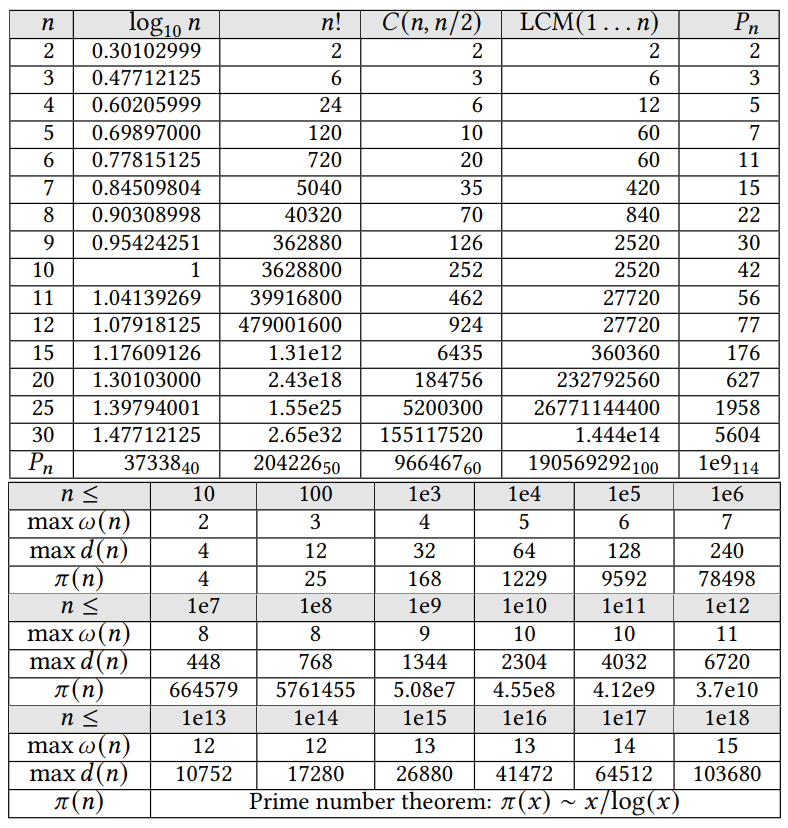
\includegraphics[width=0.8\textwidth]{contents/0x10 基础/figures/0x11 常数表.png}
\end{center}

\subsection{常用公式}

\subsubsection{日期公式}

\InputCode{cpp}{contents/0x10 基础/code/0x11 日期公式.cpp}

\subsubsection{xorshift}

\InputCode{cpp}{contents/0x10 基础/code/0x11 xorshift.cpp}

\subsubsection{xorsum}

\[
\operatorname{xor}_{i = 1}^n i = \begin{cases}
n, & n \bmod 4 = 0 \\
1, & n \bmod 4 = 1 \\
n + 1, & n \bmod 4 = 2 \\
0, & n \bmod 4 = 3
\end{cases}
\]

\InputCode{cpp}{contents/0x10 基础/code/0x11 xorsum.cpp}

\subsubsection{Sum of Powers}

\[
\begin{gathered}
\sum_{i = 1}^n i^2 = \frac{n(n + 1)(2n + 1)}{6}, \quad \sum_{i = 1}^n i^3 = \left( \frac{n(n + 1)}{2} \right)^2 \\
\sum_{i = 1}^n i^4 = \frac{n(n + 1)(2n + 1)(3n^2 + 3n - 1)}{30} \\
\sum_{i = 1}^n i^5 = \frac{n^2(n + 1)^2(2n^2 + 2n - 1)}{12}
\end{gathered}
\]

\subsection{常用配置}

\subsubsection{makefile}

\begin{minted}{make}
CXXFLAGS = -std=c++23 -O2 -Wall -fsanitize=undefined

# -D_GLIBCXX_DEBUG : STL debug mode
# -fsanitize=address : 内存错误检查
# -fsanitize=undefined : UB 检查
\end{minted}

\subsubsection{pragma}

\begin{minted}{cpp}
#pragma GCC optimize("O3,unroll-loops")
#pragma GCC target("avx2")
\end{minted}

\subsubsection{ulimit}

\begin{minted}{bash}
ulimit -s 1048576
\end{minted}

\subsubsection{Linux 对拍脚本}

需要 \texttt{chmod +x cmp.sh}，然后才能 \texttt{./cmp.sh}。

\begin{minted}{bash}
while true; do
    ./gen >0.in
    ./obj <0.in >1.out
    ./std <0.in >2.out
    let cnt=cnt+1; echo "Test $cnt:"
    if diff 1.out 2.out; then
        echo ac
    else
        echo wa
        break;
    fi
done
\end{minted}

\subsubsection{Windows 对拍程序}

\begin{minted}{cpp}
#include <bits/stdc++.h>
int main() {
    int T = 100;
    for (int i = 1; i <= T; i ++) {
        system("gen.exe >0.in");
        system("obj.exe <0.in >1.out");
        system("std.exe <0.in >2.out");
        std::cout << "Test " << i << ":\n";
        if (system("fc 1.out 2.out")) {
            std::cout << "wa\n";
            break;
        } else {
            std::cout << "ac\n";
        }
    }
}
\end{minted}

\subsection{随机数据生成}

\subsubsection{生成区间 [l,r] 中的随机整数}

\InputCode{cpp}{contents/0x10 基础/code/0x11 生成区间 [l,r] 中的随机整数.cpp}

\subsubsection{生成区间 [l,r) 中的随机浮点数}

\InputCode{cpp}{contents/0x10 基础/code/0x11 生成区间 [l,r) 中的随机浮点数.cpp}

\subsubsection{生成互不相同的随机整数}

\InputCode{cpp}{contents/0x10 基础/code/0x11 生成互不相同的随机整数.cpp}

\subsubsection{生成随机树}

\begin{itemize}
\item 均匀随机树的期望直径为 $\mathcal{O}(\sqrt{n})$ 级别。
\end{itemize}

\InputCode{cpp}{contents/0x10 基础/code/0x11 生成随机树.cpp}

\subsection{常用库函数重载}

\subsubsection{i128}

重载了 \texttt{\_\_int128} 的标准输入输出流。

\InputCode{cpp}{contents/0x10 基础/code/0x11 i128.cpp}

\subsubsection{整数除法精确取整}

\InputCode{cpp}{contents/0x10 基础/code/0x11 整数除法精确取整.cpp}

\subsubsection{取最值}

\InputCode{cpp}{contents/0x10 基础/code/0x11 取最值.cpp}

\subsubsection{取模}

\InputCode{cpp}{contents/0x10 基础/code/0x11 取模.cpp}

\subsubsection{精确开根号}

\InputCode{cpp}{contents/0x10 基础/code/0x11 精确开根号.cpp}

\subsubsection{精确取对数}

\InputCode{cpp}{contents/0x10 基础/code/0x11 精确取对数.cpp}

\subsubsection{快读}

\InputCode{cpp}{contents/0x10 基础/code/0x11 快读.cpp}

\subsubsection{超级快读}

\InputCode{cpp}{contents/0x10 基础/code/0x11 超级快读.cpp}

\subsection{高精度}

\InputCode{cpp}{contents/0x10 基础/code/0x11 高精度.cpp}

\subsection{分数类}

\InputCode{cpp}{contents/0x10 基础/code/0x11 分数类.cpp}



\section{0x12\ 基础\ 算法}
\label{sec:0x12}

\subsection{主定理}

\Highlight{主定理}：用于求解分治递归类型的渐进时间复杂度问题。

具体地，对于一个规模为 $n$ 的问题，将其划分成 $a$ 个规模为 $\frac{n}{b}$ 的子问题，附带 “合并/分割” 的开销 $f(n)$。
\[
T(n) = aT\left( \frac{n}{b} \right) + f(n)
\]

\textbf{以 $n^{\log_b a}$ 为处理问题用时的基准线。}

\begin{itemize}
\item 若 $f(n) = O(n^{\log_b a - \epsilon})$\newline{}
\textbf{直觉：总工作量由 “叶子层” 主导。}
\[
T(n) = \Theta(n^{\log_b a})
\]

\item 若 $f(n) = \Theta(n^{\log_b a}\log^k n)$ 且满足 $k\geq 0$\newline{}
\textbf{直觉：每一层工作量相近，共 $\log_b n$ 层。}
\[
T(n) = \Theta(n^{\log_b a}\log^{k + 1} n)
\]

\item 若 $f(n) = \Omega(n^{\log_b a + \epsilon})$ 且满足正则性条件 $af(\frac{n}{b}) \leq cf(n)$（其中 $c < 1$）\newline{}
\textbf{直觉：总工作量由顶层的 合并/分割 主导。}
\[
T(n) = \Theta(f(n))
\]
\end{itemize}

\begin{quoteblock}
一些例子：

\begin{itemize}
\item 情形 1：遍历满二叉树 $T(n) = 2T(\frac{n}{2}) + O(1) = O(n)$。
\item 情形 2：归并排序 $T(n) = 2T(\frac{n}{2}) + O(n) = \mathcal{O}(n \log n)$。
\item 情形 3：多项式牛顿迭代 $T(n) = T(\frac{n}{2}) + \mathcal{O}(n \log n) = \mathcal{O}(n \log n)$。
\end{itemize}

一个主定理处理不了的例子：$T(n) = 2T\left(\frac{n}{2}\right) + \mathcal{O}\left(\frac{n}{\log n}\right) = \mathcal{O}(n \log \log n)$。
\end{quoteblock}

\subsection{快速乘}

求解 $a \times b \bmod p$，其中 $a, b, p$ 均为 \texttt{long long} 范围。

正道正确率更高，魔道效率更高。

\subsubsection{正道：i128}

\InputCode{cpp}{contents/0x10 基础/code/0x12 快速乘（i128）.cpp}

\subsubsection{魔道：long double}

注意到 $a\times b \bmod p = a\times b - \lfloor \frac{a \times b}{p} \rfloor\times p$，利用 \texttt{long double} 来处理 $\lfloor \frac{a \times b}{p} \rfloor$。

\textbf{模数较大时可能会出锅。}

\InputCode{cpp}{contents/0x10 基础/code/0x12 快速乘（long double）.cpp}

\subsection{光速幂}

对于一个\textbf{固定底数} $a$，多次询问 $a^i \bmod p$ 的值（其中 $0 \leq i \leq n$）。

取阈值 $B = \left\lceil \sqrt{n} \right\rceil$，先预处理出 $a^1, a^2, \dots, a^i, \dots, a^B$，再预处理出 $a^B, a^{2B}, \dots, a^{iB}, \dots, a^{\lfloor n / B \rfloor B}$。

每次只需利用 $a^i = a^{\lfloor i / B \rfloor B}\times a^{i \bmod B}$ 回答询问即可。

时间复杂度：预处理 $\mathcal{O}(\sqrt{n})$，查询 $\mathcal{O}(1)$。

\begin{quoteblock}
$k$ 进制快速幂：利用 $a^i = \left( a^k \right)^{\lfloor i / k \rfloor} \times a^{i \bmod k}$ 递归处理询问（右侧预处理，左侧递归）。

时间复杂度：预处理 $\mathcal{O}(k \log_k n)$，查询 $\mathcal{O}(\log_k n)$。
\end{quoteblock}

\InputCode{cpp}{contents/0x10 基础/code/0x12 光速幂.cpp}



\section{0x21\ 字符串\ I}
\label{sec:0x21}

\subsection{哈希}

\subsubsection{字符串哈希}

\Highlight{字符串哈希}：字符串哈希要求\textbf{数据有序}。将字符串的元素通过某种\textbf{不具有交换律的运算}结合（例如字符串拼接，矩阵乘法 ...）。

通常将字符串 $s$ 视为一个 \textbf{$\mathrm{base}$ 进制数}，即
\[
f(s) \equiv \sum_{i = 1}^{l} s_i \times \mathrm{base}^{l - i} \pmod M
\]

其中模数 $M$ 尽量为\textbf{大质数}，并且尽量对两个大质数模数 $M_1, M_2$ 各求一次哈希（\textbf{双哈希}）

\Highlight{静态字符串区间哈希}：
\[
\begin{gathered}
\mathrm{pre}_i = \mathrm{pre}_{i - 1} \times \mathrm{base} + s_i \\
f(s[l : r]) = \mathrm{pre}_r - \mathrm{pre}_{l - 1} \times \mathrm{base}^{r - l + 1}
\end{gathered}
\]

\Highlight{动态字符串区间哈希}：区间哈希值可以合并。设左右两个区间的长度与哈希值分别为 $(l_1, h_1), (l_2, h_2)$，将它们拼接形成大区间的长度与哈希值为
\[
(l_1 + l_2, h_1 \times \mathrm{base}^{l_2} + h_2)
\]

可以使用线段树动态维护。

\Highlight{卡自然溢出哈希（Hash Killer I）}：

$\mathrm{base}$ 为偶数：此时 $\mathrm{base}^{64} \equiv 0 \pmod{2^{64}}$。所以两个长度 $> 64$，且后 $64$ 位相同的不完全相同字符串就会哈希冲突。

$\mathrm{base}$ 为奇数：使用 Thue Morse 序列攻击。对于二进制串 $s$，设 $\overline{s}$ 表示 $s$ 按位取反后得到的串。

Thue Morse 序列：$t_0 = \mathtt{0}$，$t_i = t_{i - 1} + \overline{t_{i - 1}}$。此时
\[
\begin{gathered}
f(t_i) = \mathrm{base}^{2^{i - 1}} f(t_{i - 1}) + f(\overline{t_{i - 1}}) \\
f(\overline{t_i}) = \mathrm{base}^{2^{i - 1}} f(\overline{t_{i - 1}}) + f(t_{i - 1})
\end{gathered}
\]

记 $h_i = f(t_i) - f(\overline{t_i})$，有 $h_i = \left(\mathrm{base}^{2^{i - 1}} - 1\right)h_{i - 1}$。由于
\[
\mathrm{base}^{2^{i - 1}} - 1 = (\mathrm{base}^{2^{i - 2}} + 1)(\mathrm{base}^{2^{i - 3}} + 1)\dots(\mathrm{base} + 1)(\mathrm{base} - 1)
\]

其中每一项都是偶数，所以 $2^i \mid \mathrm{base}^{2^{i - 1}} - 1$。于是 $2^{\frac{i(i + 1)}{2}} \mid h_i$，因此 $t_{11}$ 与 $\overline{t_{11}}$ 就会哈希冲突。

\begin{quoteblock}
Thue Morse 序列的规律：第 $x$ ($x \geq 0$) 位上的值等于 $\mathrm{popcount}(x) \bmod 2$。
\end{quoteblock}

\Highlight{卡大质数哈希（Hash Killer II）}：使用生日悖论攻击。

\subsubsection{集合哈希}

\Highlight{集合哈希}：集合哈希要求\textbf{数据无序}。将集合的元素通过某种映射规则转化后，再通过某种\textbf{具有交换律的运算}结合。

\Highlight{可用的映射规则}：以打乱原来可能有的某些性质。

\begin{itemize}
\item 查表映射：将原数值 $x$ 随机赋一个新数值 $c_x$ 并存入表中。
\end{itemize}

\Highlight{可用的结合方式}：

\begin{itemize}
\item 使用加法结合：
\[
f(S) = \sum_{x \in S} \mathrm{shift}(x)
\]

\item 使用异或结合（\textbf{异或哈希}）：
\[
f(S) = \bigoplus_{x \in S} \mathrm{shift}(x)
\]
\end{itemize}

此时出现偶数次元素无贡献，出现奇数次元素只贡献一次。

\Highlight{异或哈希判完全平方数}：定义\textbf{完全异或性}函数 $f$，对于任意正整数 $x, y$ 都有 $f(xy) = f(x) \oplus f(y)$。先对 $1 \sim n$ 进行一次线性筛。给其中的所有质数 $p$ 对应的 $f(p)$ 赋一个范围较大的随机数，其余合数的 $f$ 值通过线性筛得出。

\textbf{此时 $x$ 为完全平方数，当且仅当 $f(x) = 0$}。

当待判断的数可以表示为若干个 $[1, n]$ 范围内整数的乘积时，就可以根据这些数的 $f$ 函数异或和求出该数的 $f$ 函数，从而快速判断其是否为完全平方数。

\subsection{kmp}

\Highlight{字符串的 border}：对字符串 $s$ 与整数 $0 \leq r < |s|$，若 $s$ 长度为 $r$ 的前缀与后缀相等，则称 $s$ 长度为 $r$ 的前缀为 $s$ 的 border。

\Highlight{字符串的周期}：对字符串 $s$ 与整数 $1 \leq p \leq |s|$，若对于任意 $i \in [1, |s| - p]$ 均有 $s_i = s_{i + p}$，则称 $p$ 为 $s$ 的周期。特别地，若 $p$ 整除 $|s|$，则称 $p$ 为 $s$ 的整周期。

相当于 $s[1 : n - p] = s[p + 1 : n]$，所以 \textbf{$s$ 有长度为 $r$ 的 border $\iff$ $|s| - r$ 是 $s$ 的周期}。

\Highlight{kmp}：记 $\mathrm{next}_i$ 表示字符串 $s[1 : i]$ 的最长 border 的长度。

利用 border 的 border 还是原串 border 的性质，可以 $\mathcal{O}(n)$ 求解前缀函数。

进一步，\textbf{$s[1 : i]$ 的所有 border 为 $\mathrm{next}_i, \mathrm{next}_{\mathrm{next}_i}, \dots$}

\InputCode{cpp}{contents/0x20 字符串/code/0x21 kmp.cpp}

\subsubsection{border 理论}

\Highlight{弱周期引理}：若 $p, q$ 是 $s$ 的周期且 $p + q \leq n$，则 $\gcd(p, q)$ 也是 $s$ 的周期。

证明：不妨设 $p > q$，下面证明 $p - q$ 也是 $s$ 的周期。

\begin{itemize}
\item 当 $i \leq q$ 时，$s_i = s_{i + p} = s_{i + p - q}$。
\item 当 $i > q$ 时，$s_i = s_{i - q} = s_{i + p - q}$。
\end{itemize}

所以 $p - q$ 也是 $s$ 的周期，运用辗转相除法可知 $\gcd(p, q)$ 也是 $s$ 的周期。

\begin{quoteblock}
周期引理：若 $p, q$ 是 $s$ 的周期且 $p + q - \gcd(p, q) \leq n$，则 $\gcd(p, q)$ 也是 $s$ 的周期。
\end{quoteblock}

\Highlight{长 border 结构}：$s$ 的所有长度 $\geq \left\lfloor\frac{n}{2}\right\rfloor$ 的 border，它们与 $n$ 共同构成一个等差数列，公差为 $s$ 的最小周期。

证明：对于两个不同 border $n - p, n - q$ ($p, q \leq \left\lceil \frac{n}{2} \right\rceil$)，\textbf{其中 $n - p$ 是最大的 border}。

已知 $p, q$ 是 $s$ 的周期，由于 $p + q \leq n$，可知 $\gcd(p, q)$ 也是 $s$ 的周期。由于 $n - p$ 是最大 border，所以 $p$ 是最小周期。结合两个条件可得 $\gcd(p, q) = p$，即 $p \mid q$。同时，周期的整数倍也一定是周期。

综上，$s$ 的所有长度 $\geq \left\lfloor\frac{n}{2}\right\rfloor$ 的 border 与 $n$ 共同构成一个\textbf{公差为 $p$（最小周期）的等差数列}。

\begin{quoteblock}
短周期结构：$s$ 的所有长度 $\leq \left\lceil \frac{n}{2} \right\rceil$ 的周期，都是 $s$ 最小周期的倍数。

证明同「长 border 结构」。
\end{quoteblock}

\Highlight{字符串 border 结构}：$s$ 的所有 border 可以被划分成至多 $\left\lceil \log_2 n \right\rceil$ 个等差数列。

进一步，每个等差数列都具有一定的周期性。同一个等差数列里的字符串，都可以被表示成
\[
W, W + A, W + A^2, \dots, W + A^k
\]

或
\[
W, B + W, B^2 + W, \dots, B^k + W
\]

其中 $W, A, B$ 均为字符串。

证明：设 $[2^i, 2^{i + 1})$ 中最大的 border 为 $p$，那么段内的其余 border 都是 $s[1 : p]$ 的 border，且长度 $\geq \left\lfloor \frac{p}{2} \right\rfloor$，由「长 border 结构」可知段内构成一个等差数列。

推论：$s$ 的所有公差 $\geq d$ 的 border 的等差数列总大小是 $\mathcal{O}\left( \frac{n}{d} \right)$ 的。

\Highlight{Misc}：

\begin{itemize}
\item 若 $s$ 在 $t$ 中的某两个匹配 $s_1, s_2$ 有重合，且起始位置相差 $d$，则 $d$ 均为 $s$ 与 $s_1 \cup s_2$（两个匹配区间并）的周期。
\item 若 $|s| \geq \frac{|t|}{2}$，则 $s$ 在 $t$ 中的匹配起始位置形成等差数列。若该等差数列至少有 $3$ 项，则公差为 $s$ 的最小周期 $\mathrm{per}(s)$。
\end{itemize}

\subsection{Z Algorithm}

\Highlight{Z Algorithm}：记 $Z_i$ 表示字符串 $s$ 与 $s[i : n]$ 的最长公共前缀（LCP）长度。在某些情况下，可能会记 $Z_1 = 0$。

考虑从前向后扫。维护一个右端点最靠右，且与 $s$ 的前缀匹配的子串 $s[l : r]$。

\begin{itemize}
\item 若 $i \leq r$，则
\[
Z_i \geq \min(Z_{i - l + 1}, r - i + 1)
\]

\item 若 $i > r$，则
\[
Z_i \geq 0
\]
\end{itemize}

在当前 $Z_i$ 的基础上不断尝试扩展。

注意到单次枚举的次数为 $\max\{l + Z_l - 1\}$ 的增量，时间复杂度 $\mathcal{O}(n)$。

\InputCode{cpp}{contents/0x20 字符串/code/0x21 Z-Algorithm.cpp}

\subsection{manacher}

\Highlight{奇偶回文串的处理}：回文串按照长度分成奇偶两类，奇回文串的对称轴处于一个字符上，偶回文串的对称轴处于两个相邻字符的中间。

可以在一个字符串的首尾以及所有的相邻两字符之间，插入一个原串中从未出现的字符（例如 \texttt{\#}, \texttt{\$}, \texttt{\textasciicircum{}}）。

这样原串中的每一个回文串，都可以对应到新串中的一个两端都是分隔符的奇回文串。

\Highlight{manacher}：记 $p_i$ 表示以位置 $i$ 为中心的最长回文子串的半径（含中心）。

考虑从前向后扫。维护一个右端点最靠右的回文子串，不妨记该回文串的中心为 $k$。

\begin{itemize}
\item 若 $i \leq k + p_k - 1$，则
\[
p_i \geq \min(k + p_k - i, p_{2k - i})
\]

\item 若 $i > k + p_k - 1$，则
\[
p_i \geq 0
\]
\end{itemize}

在当前 $p_i$ 的基础上不断尝试扩展。

注意到单次枚举的次数为 $\max\{k + p_k - 1\}$ 的增量，时间复杂度 $\mathcal{O}(n)$。

\InputCode{cpp}{contents/0x20 字符串/code/0x21 manacher.cpp}

\InputCode{cpp}{contents/0x20 字符串/code/0x21 manacher（奇偶分开考虑）.cpp}

\Highlight{反回文串}：对于长度为 $n$ 的字符串 $s$，若对于任意 $i \in [1, n]$ 均有 $s_i \neq s_{n - i + 1}$，则称 $s$ 为反回文串。

\Highlight{01 串的反 manacher}：相当于对于每两个相邻字符的中间，求以该位置为中心的\textbf{最长反回文子串}的半径。注意我们只需要考虑长度为偶数的串。

当字符集大小为 $2$ 时，考虑形如 \texttt{ABCD} 的字符串，若已知 $A \neq B, A \neq D, B \neq C$，可以推出 $C\neq D$，所以 manacher 的对称复用逻辑还是正确的。但是字符集大小超过 $2$ 的时候，上述推理就不成立了。

具体实现时，只需要将 manacher 偶回文串指针扩展过程中的 \texttt{==} 改成 \texttt{!=} 即可。

\subsection{Lyndon 分解}

\Highlight{Lyndon 串}：对于字符串 $s$，若 $s$ 的字典序小于 $s$ 的所有非空真后缀，则称 $s$ 为 Lyndon 串。

等价定义：

\begin{itemize}
\item 字符串 $s$ 的字典序\textbf{严格小于} $s$ 的其他循环移位。
\item 对字符串 $s$ 的任意非空分解 $s = uv$，都有 $u < v$。
\item 对字符串 $s$ 的任意非空分解 $s = uv$，都有 $uv < vu$。
\end{itemize}

\Highlight{Lyndon 串的拼接性质}：

\begin{itemize}
\item \textbf{若字符串 $u, v$ 均为 Lyndon 串并且 $u < v$，则 $uv$ 为 Lyndon 串，且 $u < uv < v$}。
\item 若字符串 $u, v$ 均为 Lyndon 串并且 $u < v$，则对于任意正整数 $a, b$，均有 $u^av^b$ 为 Lyndon 串，且 $u < u^av^b < v$。
\item 字符串 $s$ ($|s| \geq 2$) 是 Lyndon 串，当且仅当 $s = uv$ ($|u| > 0, |v| > 0, \boldsymbol{u < v}$) 并且 $u, v$ 均为 Lyndon 串。
\end{itemize}

\Highlight{Lyndon 串的简单性质}：

\begin{itemize}
\item Lyndon 串不存在非空 border。
\item 截取 Lyndon 串的某个前缀，将其末字符增大，结果仍是 Lyndon 串（截出的前缀本身不必是 Lyndon 串）。
\item 若字符串 $s_1, s_2$ 满足 $s_1$ 是 Lyndon 串且 $s_1 > s_2$，则 $s_1 > s_2^2$。
\end{itemize}

\Highlight{Lyndon 分解}：将字符串 $s$ 分解为 $w_1w_2\dots w_k$，其中所有的 $w_i$ 均为 Lyndon 串，且满足 $w_1 \geq w_2 \geq \dots \geq w_k$。

\Highlight{Lyndon 分解的性质}：

\begin{itemize}
\item Lyndon 分解存在且唯一。
\item 字符串 $s$ 的字典序最小非空后缀为 $w_k$。
\item 字符串 $s$ 是 Lyndon 串当且仅当 $k = 1$。
\end{itemize}

\Highlight{Lyndon 分解（duval）}：

\InputCode{cpp}{contents/0x20 字符串/code/0x21 duval.cpp}

\subsection{最小表示法}

\Highlight{循环同构}：若长度为 $n$ 的字符串 $s$，可以选择一个起始位置 $i$ ($1 \leq i \leq n$)，使得 $s[i : n] + s[1 : i - 1] = t$，则称 $s, t$ 循环同构。

\Highlight{最小表示法}：字符串 $s$ 的最小表示法，为与 $s$ 循环同构的所有字符串中，字典序最小的字符串。

对于两个不同的起始位置 $i, j$，已知它们的前 $k$ 位相同。考虑继续比较下一位：

\begin{itemize}
\item 若 $s_{(i + k) \bmod n} > s_{(j + k) \bmod n}$，可以发现区间 $[i, i + k]$ 内的起始位置都不能成为答案，因为\textbf{对于起始位置 $i + p$ ($p \in [0, k]$) 来说，起始位置 $j + p$ 一定更优}。所以此时可以跳过区间 $[i, i + k]$ 的起始位置，令 $i \gets i + k + 1$，$k \gets 0$。
\item 若 $s_{(i + k) \bmod n} < s_{(j + k) \bmod n}$ 也是同理，跳过区间 $[j, j + k]$ 的起始位置，令 $j \gets j + k + 1$，$k \gets 0$。
\item 若 $s_{(i + k) \bmod n} = s_{(j + k) \bmod n}$，令 $k \gets k + 1$，然后继续比较。
\end{itemize}

在跳转的过程中，若两个起始位置 $i, j$ 相同，则任选一个加一。最终 $\min(i, j)$ 即为最优的起始位置。

时间复杂度 $\mathcal{O}(n)$。

\InputCode{cpp}{contents/0x20 字符串/code/0x21 最小表示法.cpp}

\subsection{带通配符的字符串匹配}



\section{0x22\ 字符串\ II}
\label{sec:0x22}

\subsection{Trie}

\Highlight{trie}：trie 是一个纯正的自动机，形态是树。

\begin{itemize}
\item 一个起点，若干终点。
\item 多模式串的所有前缀，与 trie 上的所有状态一一对应。
\item trie 主要考虑一种转移边：表示在当前状态所表示的串后面加一个字符。
\end{itemize}

\Highlight{01 trie}：

\begin{itemize}
\item 01 trie 支持可持久化，可以作为 \textbf{01 trie 的前缀和}来使用。
\item 01 trie 支持合并：
  \begin{itemize}
  \item 01 trie 单次合并复杂度，取决于两棵 01 trie 的交集大小。
  \item 01 trie 合并总复杂度，取决于所有 01 trie 的节点总数。
  \end{itemize}
\item 01 trie 支持可持久化合并，需要在合并时新建节点。
\end{itemize}

\InputCode{cpp}{contents/0x20 字符串/code/0x22 01 trie.cpp}

\InputCode{cpp}{contents/0x20 字符串/code/0x22 可持久化 01 trie.cpp}

\Highlight{01 trie 查询与 $x$ 异或的最大值}：\textbf{从高位到低位贪心}，有异走异，无异走同。

\Highlight{01 trie 查询与 $x$ 异或的第 $k$ 大值}：\textbf{从高位到低位}

\begin{itemize}
\item 设当前考虑到第 $i$ 位，设 $x$ 的异位有 $\mathrm{cnt}$ 个数。
  \begin{itemize}
  \item 若 $k \leq \mathrm{cnt}$，则查询 $x$ 的异位中，与 $x$ 异或的第 $k$ 大值。
  \item 若 $k > \mathrm{cnt}$，则查询 $x$ 的同位中，与 $x$ 异或的第 $k - \mathrm{cnt}$ 大值。
  \end{itemize}
\end{itemize}

\Highlight{01 trie 查询与 $x$ 异或 $\geq k$ 的信息}：\textbf{从高位到低位}

\begin{itemize}
\item 设当前考虑到第 $i$ 位：
  \begin{itemize}
  \item 若 $k$ 的第 $i$ 位为 $1$，直接走 $x$ 的异位。
  \item 若 $k$ 的第 $i$ 位为 $0$，统计 $x$ 的异位的贡献，然后走 $x$ 的同位。
  \end{itemize}
\item 考虑完所有位之后，统计当前叶子节点的贡献。
\end{itemize}

\Highlight{01 trie 全局异或 $x$}：\textbf{从高位到低位}，运用懒标记。

设当前考虑到第 $i$ 位，若懒标记的第 $i$ 位为 $1$，则交换左右儿子。

\Highlight{01 trie 维护集合异或和，支持插入、删除、全局 +1}：\textbf{从低位到高位}

\begin{itemize}
\item 额外维护：
  \begin{itemize}
  \item $\mathrm{cnt}$：当前状态的子树内的节点数。
  \item $\mathrm{xr}$：当前状态的子树内的异或和。
  \end{itemize}
\item 插入、删除：递归操作即可。
\item 全局 +1：交换当前节点的左右儿子，然后进入 $0$ 转移边（未交换前是 $1$ 转移边）的儿子进行递归交换。
\end{itemize}

（因为考虑二进制下 +1，相当于是\textbf{从低位到高位}找到第一个 $0$ 将其改为 $1$，然后将前面的 $1$ 都改为 $0$）

\InputCode{cpp}{contents/0x20 字符串/code/0x22 01 trie 维护集合异或和.cpp}

\subsection{AC 自动机}

\Highlight{AC 自动机}：AC 自动机是一个状态自动机，形态是 trie。

\begin{itemize}
\item 一个起点，若干终点。
\item 多模式串的所有前缀，与 AC 自动机上的所有状态一一对应。
\item AC 自动机主要考虑两种边：
  \begin{itemize}
  \item 普通转移边：表示在当前状态所表示的串后面加一个字符。
  \item 失配指针 fail：表示当前状态所表示的串的最长匹配后缀。这类边构成一棵树，称作 fail 树。
  \end{itemize}
\end{itemize}

\Highlight{trie 图}：将原来 trie 中不存在的转移边 $\delta(p, c)$ 指向 $\delta(\mathrm{fail}_p, c)$。本质上是路径压缩。

\Highlight{trie 图的普通转移边}：从字符串 $s$ 指向 $s' + c$，其中 $s'$ 为 $s$ 中满足 $s' + c$ 存在的最长后缀。

\InputCode{cpp}{contents/0x20 字符串/code/0x22 AC 自动机.cpp}

\Highlight{AC 自动机（大字符集）}：当字符集很大时，需要用到 \texttt{std::map} 与可持久化数组建立 trie 图。

\InputCode{cpp}{contents/0x20 字符串/code/0x22 AC 自动机（大字符集）.cpp}

\Highlight{AC 自动机查询所有模式串在文本串中的出现位置}：

\textbf{将所有询问串 $t$ 去重之后}，所有询问串 $t$ 在文本串 $s$ 中的出现次数之和不超过 $\mathcal{O}(|s|\sqrt{\sum |t|})$ 级别。

因为询问串的串长 $|t|$ 种类数不超过 $\mathcal{O}(\sqrt{\sum |t|})$ 级别，同一长度的询问串 endpos 各不相同。

对询问串建 AC 自动机（trie 图），每个节点记录一下向上跳 fail 指针遇到的最近询问节点 up。

然后从左到右扫描 $s$，扫描到右端点 $r$ 时，维护以 $r$ 结尾的最长匹配串对应的状态。然后在当前状态不断地跳 up 指针，去更新（记录）当前询问串在 $s$ 中的 endpos。

\subsection{SA}

\Highlight{序列 SA 的求法}：

\begin{itemize}
\item $\mathcal{O}(n \log^2 n)$：sort + 倍增 + hash。当比较函数时间开销较大时，尝试使用 \texttt{std::stable\_sort()}。
\item $\mathcal{O}(n \log n)$：倍增 + 基数排序（双关键字排序）。
\item $\mathcal{O}(n)$：DC3，SA-IS。
\end{itemize}

\Highlight{height 数组}：$\mathrm{height}_i = \mathrm{LCP}(\mathrm{sa}_{i - 1}, \mathrm{sa}_i)$

\Highlight{height 数组求后缀 LCP}：后缀 $\mathrm{sa}_i, \mathrm{sa}_j$ ($i < j$) 的最长公共前缀为

\[
\mathrm{LCP}(\mathrm{sa}_i, \mathrm{sa}_j) = \min_{i < k \leq j}\{\mathrm{height}_k\}
\]
\Highlight{本质不同子串个数}：

\[
\frac{n(n + 1)}{2} - \sum_{i = 2}^n \mathrm{height}_i
\]

\Highlight{（序列 SA）height 数组的性质}：$\mathrm{height}_{\mathrm{rk}_i} \geq \mathrm{height}_{\mathrm{rk}_{i - 1}} - 1$

证明：

\begin{itemize}
\item 当 $\mathrm{height}_{\mathrm{rk}_{i - 1}} = 0$ 时，命题成立。
\item 当 $\mathrm{height}_{\mathrm{rk}_{i - 1}} \geq 1$ 时，考虑到后缀排序将 “前缀相近的后缀” 放到一起，所以 $\mathrm{height}_i$ 可以视为字典序小于 $\mathrm{sa}_i$ 的后缀与 $\mathrm{sa}_i$ 的 LCP 最大值。记 $u = \mathrm{sa}_{\mathrm{rk}_{i - 1} - 1}$，则有 $s_u = s_{i - 1}$，于是 $s[u + 1 : n]$ 的字典序比 $s[i : n]$ 更小，则必然存在一个字典序小于 $s[i : n]$ 的后缀使得与其的 LCP 大于等于 $\mathrm{height}_{\mathrm{rk}_{i - 1}} - 1$，故命题成立。
\end{itemize}

\InputCode{cpp}{contents/0x20 字符串/code/0x22 SA.cpp}

\subsection{SAM}

\Highlight{SAM 与其他后缀数据结构的关系}：

\begin{itemize}
\item 后缀 trie：一个字符串的所有后缀构成的 trie。
\item 后缀 trie 上建 AC 自动机的 fail 指针：表示删除当前状态所表示的串的首字母。
\item 后缀树：后缀 trie 虚树化（仅保留所有后缀在后缀 trie 上的终止节点，以及两两 LCA）。
\item 后缀自动机的 parent 树：反串的后缀树。
\end{itemize}

\Highlight{SAM}：SAM 是一个状态自动机，形态是 DAG。

\begin{itemize}
\item 一个起点，若干终点。
\item 原串的所有本质不同的子串，与在 SAM 上从起点开始到任意点结束的所有路径一一对应，不重不漏。
\item SAM 主要考虑两种边：
  \begin{itemize}
  \item 普通转移边：表示在当前状态所表示的串后面加一个字符。
  \item 后缀链接 link：表示将当前状态所表示的最短串的首字母删除。这类边构成一棵树，称作 parent 树。
  \end{itemize}
\item SAM 点数 $\leq 2n - 1$，边数 $\leq 3n - 4$。
\end{itemize}

\Highlight{endpos 集合}：子串 $s$ 的所有终止位置的集合，记做 $\mathrm{endpos}(s)$。

\begin{itemize}
\item SAM 中的每一个状态，都对应一个 endpos 等价类。
\item SAM 中的每一个状态（endpos 等价类），包含的子串长度构成一个连续段，且短串是长串的后缀。
\item 若 $s_1$ 为 $s_2$ 的后缀，则 $\mathrm{endpos}(s_1) \supseteq \mathrm{endpos}(s_2)$；否则 $\mathrm{endpos}(s_1) \bigcap \mathrm{endpos}(s_2) = \varnothing$。
\end{itemize}

\Highlight{endpos 集合的维护}：在 parent 树上使用\textbf{（可持久化）线段树合并}维护。

由于在 parent 树上，节点 $p$ 的 endpos 集合为 $\mathrm{subtree}(p)$ 中所有节点 endpos 集合的并集。为此，我们\textbf{在 $s[1 : i]$ 对应状态的 endpos 集合里插入位置 $i$，然后使用数据结构合并子树的 endpos 集合}。

当字符集很大时，需要用到 \texttt{std::map} 建立 SAM。

\InputCode{cpp}{contents/0x20 字符串/code/0x22 SAM.cpp}

\Highlight{SAM 子串定位}：\textcolor{blue}{求 $s[l : r]$ 在 SAM 中的对应状态}

先定位 $s[1 : r]$ 在 SAM 中的对应状态（在构造 SAM 的过程中记录一下），然后\textbf{在 parent 树上倍增}，找到深度最浅的满足 $\mathrm{maxl} \geq r - l + 1$ 的状态。

\Highlight{SAM 子串匹配}：\textcolor{blue}{给定模式串 $S$ 与文本串 $T$，对每个右端点~$r$ 求最左端的 $l$ 使得 $T[l : r]$ 为 $S$ 的子串}

当 $r$ 扩展时，不断地跳后缀链接（这里令 $\mathrm{len}$ 变为对应状态的 $\mathrm{maxl}$），直到跳到根节点或存在相应的转移边为止。

若存在相应的转移边，则走该转移边（这里令 $\mathrm{len} \gets \mathrm{len} + 1$）。

\begin{minted}{cpp}
int p = 1, len = 0; // 当前匹配到的状态与长度
for (int i = 1; i <= m; i ++) {
    int c = T[i] - 'a';
    while (p > 1 && !SAM::t[p].trans[c]) {
        p = SAM::t[p].link, len = SAM::t[p].maxl;
    }
    if (SAM::t[p].trans[c]) {
        p = SAM::t[p].trans[c], len ++;
    }
    // 此时的 p 与 len，就是以 i 为结尾时匹配到的最长状态与长度
}
\end{minted}

\Highlight{子 SAM}：\textcolor{blue}{给定模式串 $S$ 与文本串 $T$，让 $T$ 在 $S[l : r]$ 中进行匹配}

判断由 $S[l : r]$ 组成的子 SAM 是否存在相应的转移边，首先在原 SAM 就要存在相应的转移边，并且原 SAM 中新状态的 endpos 集合在区间 $[l + \mathrm{len}' - 1, r]$ 中至少要有一个元素。

失配时，应先尝试 $\mathrm{len} \gets \mathrm{len} - 1$ 然后继续匹配，而非直接跳失配链接。

\Highlight{SAM 前端删除}：\textcolor{blue}{在一个状态的前面删除字符，求新状态}

若当前长度等于当前状态的 $\mathrm{minl}$，则跳后缀链接。

\Highlight{SAM 前端插入}：\textcolor{blue}{在一个状态的前面添加字符，求新状态}

维护每个状态 $u$ 对应 endpos 集合的任意一个元素 $\mathrm{pos}_u$，就可以做到\textbf{在原串中定位状态 $u$}。

\begin{itemize}
\item 若长度等于当前状态的 $\mathrm{maxl}$：则相当于\textbf{在 parent 树上向某一个儿子走}。在构建 parent 树的时候，预处理每个状态的极长串前加一个字符 $c$，能走到哪个儿子即可（枚举 $u$ 以及其儿子 $v$，根据 $\mathrm{pos}_v$ 在原串中定位，即可得知从 $u$ 到 $v$ 需要添加什么字符）。
\item 若长度小于当前状态的 $\mathrm{maxl}$：相当于要考虑当前状态是否能够容纳新串，根据 $\mathrm{pos}_u$ 在原串中定位，判断新加的字符是否与原串对应位置上的字符匹配。
\end{itemize}

\InputCode{cpp}{contents/0x20 字符串/code/0x22 SAM 前端操作.cpp}

\Highlight{SAM 补节点}：\textcolor{blue}{在 parent 树中，补充询问对应的状态}

parent 树是反串的后缀树，而后缀树又是后缀 trie 虚树化（仅保留所有后缀在后缀 trie 上的终止节点，以及两两 LCA）。

由于询问串 $s[l : r]$ 在 SAM 上的状态可能不完全覆盖 $\mathrm{minl} \sim \mathrm{maxl}$（为该区间的一个前缀），于是我们离线将所有询问串在 SAM 上的状态找出来，然后将状态划分，\textbf{建立有关询问串的虚拟节点（补充有关询问串的虚树结构）}。此时所有询问串一定完整地覆盖了从当前状态到根的路径，且总节点数不超过 $2n + m$。

简化了 parent 树的结构，降低了讨论难度。

\Highlight{广义 SAM}：\textcolor{blue}{对多模式串建立 SAM}

\InputCode{cpp}{contents/0x20 字符串/code/0x22 广义 SAM（离线）.cpp}

\InputCode{cpp}{contents/0x20 字符串/code/0x22 广义 SAM（在线）.cpp}

\subsection{PAM}

\Highlight{PAM}：PAM 是一个状态自动机，形态为由两棵树构成的森林。

\begin{itemize}
\item 两个起点（偶根为 $0$，奇根为 $1$），若干终点。
\item 原串的所有本质不同的回文子串，与 PAM 上的所有状态一一对应，不重不漏。
\item PAM 主要考虑两种边：
  \begin{itemize}
  \item 普通转移边：表示在当前状态所表示的串\textbf{前后各加一个字符}。
  \item 后缀链接 link：表示当前状态所表示的串的\textbf{最长回文后缀}。这类边构成一棵树，称作 parent 树。
  \end{itemize}
\item 偶根的 link 指向奇根，而我们不关心奇根的 link（因为奇根不可能失配，奇根转移出的下一个状态是单个字符，必定为回文串）。
\item PAM 点数（\textbf{本质不同回文子串个数}）$\leq n$。因为在任意串后面加一个字符，由反证法可知本质不同回文子串至多 $+1$。
\end{itemize}

\InputCode{cpp}{contents/0x20 字符串/code/0x22 PAM.cpp}

\Highlight{PAM half 指针}：表示当前状态所表示的串，长度小于等于该串一半的\textbf{最长回文后缀}。

\InputCode{cpp}{contents/0x20 字符串/code/0x22 PAM half.cpp}

\subsubsection{Palindrome Series}

当 $t$ 是回文串 $s$ 的后缀时，$t$ 是 $s$ 的 border $\iff$ $t$ 是回文串。

所以\textbf{回文串 $s$ 的回文后缀一定是 border，反之亦然}。

\Highlight{Palindrome Series}：回文串 $s$ 的所有回文后缀，可以被划分成至多 $\left\lceil \log_2 n \right\rceil$ 个等差数列。

进一步，每个等差数列都具有一定的周期性。同一个等差数列里的字符串，都可以被表示成

\[
W, W + A, W + A^2, \dots, W + A^k
\]

或

\[
W, B + W, B^2 + W, \dots, B^k + W
\]

其中 $W, A, B$ 均为字符串。

\Highlight{PAM series-link}：对于 PAM 上的每个状态 $u$

\begin{itemize}
\item $\mathrm{diff}_u = \mathrm{len}_u - \mathrm{len}_{\mathrm{link}_u}$。
\item $\mathrm{slink}_u$ 表示 $u$ 不断跳后缀链接 link，跳到的第一个满足 $\mathrm{diff}_v \neq \mathrm{diff}_u$ 的节点 $v$。
\end{itemize}

我们称 \textbf{diff 值相同的连续 link 链为一个 Series}，Series 中的回文串长度都构成一个等差数列。那么 $\mathrm{slink}_u$ 就表示 $u$ 所在的 Series 对应的下一个 Series 的最长回文节点。

上述理论可以用来优化一类 dp 问题：

\[
f_i = \bigoplus_{s[j + 1 : i] \ \text{is} \ \text{Palindrome}} f_j
\]

（其中 $\oplus$ 表示一种运算，例如 $+$ 或者 $\min$）

考虑将一个 Series 表示的所有回文串的 dp 值都记录到最长的回文串上，设 $g_u$ 表示 $u$ 所在 Series 的 dp 贡献之和（其中 $u$ 作为该 Series 中最长回文节点）。

若节点 $u$ 最近一次在位置 $i$ 结尾，且 $\mathrm{diff}_u = \mathrm{diff}_{\mathrm{link}_u}$，则 $\mathrm{link}_u$ 在严格早于 $i$ 的最近一次出现在位置 $i - \mathrm{diff}_u$ 结尾。

假设当前处理到位置 $i$，沿着 slink 处理每一个 Series 的贡献。设当前节点为 $u$，则 $u$ 所在 Series 中最短回文串长度为 $\mathrm{diff}_u + \mathrm{len}_{\mathrm{slink}_u}$，除了最短回文串的其他贡献，恰好等于在位置 $i - \mathrm{diff}_u$ 时已经维护好的 $g_{\mathrm{link}_u}$。因此有转移：

\[
g_u = \begin{cases}
f_{i - \mathrm{diff}_u - \mathrm{len}_{\mathrm{slink}_u}} & \mathrm{diff}_u \neq \mathrm{diff}_{\mathrm{link}_u} \\
f_{i - \mathrm{diff}_u - \mathrm{len}_{\mathrm{slink}_u}} \oplus g_{\mathrm{link}_u} & \mathrm{diff}_u = \mathrm{diff}_{\mathrm{link}_u}
\end{cases}
\]
\InputCode{cpp}{contents/0x20 字符串/code/0x22 PAM series-link.cpp}


\section{0x31\ 数学\ 多项式}
\label{sec:0x31}

\subsection{拉格朗日插值}

\Highlight{多项式的插值}：给出 $n + 1$ 个点 $(x_1, y_1), (x_2, y_2), \dots, (x_{n + 1}, y_{n + 1})$，\textbf{其中横坐标（模意义下）两两不同}。求一个\textbf{至多 $n$ 次}的多项式，使得这 $n + 1$ 个点都在 $f(x)$ 上。

\Highlight{拉格朗日插值}：

\[
f(x) = \sum\limits_{i = 1}^{n + 1} y_i \prod\limits_{j \neq i} \frac{x - x_j}{x_i - x_j}
\]

可以发现 $f(x)$ 是一个\textbf{至多 $n$ 次}的多项式，并且可以证明\textbf{拉格朗日插值是唯一的插值多项式}。

朴素实现的时间复杂度为 $\mathcal{O}(n^2)$，可以使用多项式优化到 $\mathcal{O}(n \log^2 n)$（详见多项式快速插值）。

\begin{quoteblock}
构造方法：考虑构造 $n + 1$ 个函数，\textbf{其中第 $i$ 个函数 $f_i(x)$ 的图像经过 $(x_i, y_i)$，对于其他的 $j \neq i$ 经过 $(x_j, 0)$}。则我们要求的 $f(x)$ 即为这 $n + 1$ 个函数的和 $\sum_{i = 1}^{n + 1} f_i(x)$。

尝试构造 $f_i(x) = a_i\prod_{j \neq i}(x - x_j)$，其中 $a_i$ 是待定的系数。此时对于 $j \neq i$ 均有 $f_i(x_j) = 0$。代入 $f_i(x_i) = y_i$ 即可解得 $a_i = \frac{y_i}{\prod_{j \neq i}(x_i - x_j)}$。

于是原式得证。
\end{quoteblock}

\InputCode{cpp}{contents/0x30 数学/code/0x31 拉格朗日插值.cpp}

\Highlight{拉格朗日插值求系数}：相当于是直接将整个多项式求出来。运用了\textbf{暴力除以单项式}的技巧。

\begin{itemize}
\item 记系数部分 $a_i = \frac{y_i}{\prod_{j \neq i} (x_i - x_j)}$。
\item 记多项式 $g(x) = \prod_{j} (x - x_j)$，记多项式 $h_i(x) = \prod_{j \neq i} (x - x_j)$。
\item 先 $\mathcal{O}(n^2)$ 暴力多项式乘法求出 $g(x)$。\textbf{考虑由 $g(x)$ 得到 $h_i(x)$，相当于是多项式 $g(x)$ 除以一个单项式 $(x - x_i)$}，仍然可以 $\mathcal{O}(n)$ 暴力除以单项式。具体地，由于 $(x - x_i)h_i(x) = g(x)$，则对于 $g(x)$ 的 $j$ ($j \geq 1$) 次项系数，有 $[x^{j - 1}]h_i - x_i[x^j]h_i = [x^j]g$。于是

\[
\begin{gathered}
[x^n]h_i = [x^{n + 1}]g \\
[x^j]h_i = [x^{j + 1}]g + x_i[x^{j + 1}]h_i \\
\end{gathered}
\]

\item 求出了 $a_i$ 与 $h_i(x)$ 之后，计算 $f(x) = \sum_{i = 1}^{n + 1}a_ih_i(x)$。时间复杂度 $\mathcal{O}(n^2)$。
\end{itemize}

\InputCode{cpp}{contents/0x30 数学/code/0x31 拉格朗日插值求系数.cpp}

\Highlight{\textbf{连续点值}的拉格朗日插值}：给出 $n + 1$ 个连续点值 $f(1), f(2), \dots, f(n + 1)$，代入拉格朗日插值公式，得

\[
f(x) = \sum\limits_{i = 1}^{n + 1}y_i \prod\limits_{j \neq i}\frac{x - j}{i - j}
\]

现在考虑给定一个自变量 $x$，求出因变量 $f(x)$。考虑右边的乘积项怎么求

\begin{itemize}
\item 分子：记 $\mathrm{pre}_i = \prod_{1 \leq j \leq i} (x - j)$，$\mathrm{suf}_i = \prod_{i \leq j \leq n + 1} (x - j)$，则分子为 $\mathrm{pre}_{i - 1} \times \mathrm{suf}_{i + 1}$。
\item 分母：$j < i$ 的部分\textbf{是 $i - 1$ 到 $1$ 乘起来}。$j > i$ 的部分\textbf{是 $-1$ 到 $-(n + 1 - i)$ 乘起来}。故分母为 $(i - 1)! (n + 1 - i)! (-1)^{n + 1 - i}$。
\end{itemize}

故最后的式子为

\[
f(x) = \sum\limits_{i = 1}^{n + 1}y_i \frac{\mathrm{pre}_{i - 1} \times \mathrm{suf}_{i + 1}}{(i - 1)!(n + 1 - i)!(-1)^{n + 1 - i}}
\]

求出单个点值的时间复杂度为 $\mathcal{O}(n)$。

\begin{quoteblock}
若给出 $n + 1$ 个连续点值 $f(h), f(h + 1), \dots, f(h + n)$，分母的求法是完全不变的，只需将分子改成 $x - x_j$ 相乘即可。

或者可以考虑将坐标系向左平移 $h - 1$。
\end{quoteblock}

\InputCode{cpp}{contents/0x30 数学/code/0x31 连续点值的拉格朗日插值.cpp}

\subsection{FFT}

\Highlight{单位根}：$n$ 次单位根，即为 $x^n = 1$ 的所有复数解。单位圆上辐角为 $0, \frac{2\pi}{n}, \frac{4\pi}{n}, \dots, \frac{2(n - 1)\pi}{n}$ 的复数都是单位根，共 $n$ 个。这些单位根依次表示为

\[
\omega_n^0, \omega_n^1, \omega_n^2, \dots, \omega_n^{n - 1}
\]
\Highlight{单位根的简单性质}：欧拉公式：$e^{ix} = \cos(x) + i \sin(x)$。这说明 $x \in \mathbb{R}$ 时，$e^{ix}$ 可以描述一个单位圆上辐角为 $x$ 的复数。

\begin{itemize}
\item $\omega_n^1 = e^{\frac{2\pi i}{n}} = \cos(\frac{2\pi}{n}) + i \sin(\frac{2\pi}{n})$。
\item $\omega_n^i \times \omega_n^j = \omega_n^{i + j}$。
\item $\left(\omega_n^i\right)^j = \omega_n^{ij}$。
\item $\omega_{2n}^{2k} = \omega_n^k$。
\item $\omega_{2n}^k = -\omega_{2n}^{k + n}$。
\end{itemize}

\Highlight{补充界}：在进行 FFT 之前，需要对其最高位补 $0$，将其补成一个最高次数为 $2^P - 1$ 的多项式。方便后续的奇偶性分组。

\subsubsection{DFT}

DFT 的思想：“系数表示法” 转 “点值表示法”。

已知系数 $a_0, \dots, a_{n - 1}$，取自变量 $\omega_n^0, \omega_n^1, \dots, \omega_n^{n - 1}$，计算点值 $F(\omega_n^0), F(\omega_n^1), \dots, F(\omega_n^{n - 1})$。

记 $n = 2^P$，考虑一个 $2^P - 1$ 次的多项式 $F(x)$

\[
F(x) = a_0 + a_1x + \dots + a_{n - 1}x^{n - 1}
\]
将每一项按照次数的奇偶性，划分成两部分（由于 $n$ 是 $2$ 的若干次幂，每次分出来的奇偶部分的次数一定相等）。

\[
F(x) = \left( a_0 + a_2x^2 + \dots + a_{n - 2}x^{n - 2} \right) + \left( a_1x + a_3x^3 + \dots + a_{n - 1}x^{n - 1} \right)
\]
记

\[
\begin{gathered}
F_L(x) = a_0 + a_2x + \dots + a_{n - 2}x^{n / 2 - 1} \\
F_R(x) = a_1 + a_3x + \dots + a_{n - 1}x^{n / 2 - 1}
\end{gathered}
\]
则

\[
F(x) = F_L(x^2)+ xF_R(x^2)
\]
考虑计算因变量 $F(\omega_n^0), F(\omega_n^1), \dots, F(\omega_n^{n - 1})$。

\begin{itemize}
\item 对于 $k < n / 2$，代入 $\omega_n^k$ 得

\[
\begin{aligned}
F(\omega_n^k) & = F_L\left((\omega_n^k)^2\right) + \omega_n^k F_R\left((\omega_n^k)^2\right) \\
& = F_L(\omega_{n / 2}^k) + \omega_n^k F_R(\omega_{n / 2}^k)
\end{aligned}
\]

\item 对于 $k < n / 2$，代入 $\omega_n^{k + n/2}$ 得

\[
\begin{aligned}
F(\omega_n^{k + n / 2}) & = F_L\left((\omega_n^{k + n / 2})^2\right) + \omega_n^{k + n / 2}F_R\left((\omega_n^{k + n / 2})^2\right) \\
& = F_L(\omega_n^{2k + n}) + \omega_n^{k + n / 2} F_R(\omega_n^{2k + n}) \\
& = F_L(\omega_{n / 2}^k) - \omega_{n}^{k} F_R(\omega_{n / 2}^k)
\end{aligned}
\]
\end{itemize}

注意到 $F(\omega_n^k), F(\omega_n^{k + n / 2})$ 等于 $F_L(\omega_{n / 2}^k) \pm \omega_n^kF_R(\omega_{n / 2}^k)$。

如果我们知道 $F_L(x), F_R(x)$ 分别在 $\omega_{n / 2}^0, \omega_{n / 2}^1, \dots, \omega_{n / 2}^{n / 2 - 1}$ 处的点值表示，就可以 $\mathcal{O}(n)$ 求出 $F(x)$ 在 $\omega_n^0, \omega_n^1, \dots, \omega_n^{n - 1}$ 处的点值表示。

这是一个分治的过程，不断分治直到仅剩一个项即可。

时间复杂度 $\mathcal{O}(n \log n)$。

\subsubsection{IDFT}

\textbf{结论：将 DFT 中的 $\omega_n^1$ 换成 $\omega_n^{-1}$，做完以后除以 $n$ 即可}。

IDFT 的思想：“点值表示法” 转 “系数表示法”。

已知点值 $F(\omega_n^0), F(\omega_n^1), \dots, F(\omega_n^{n - 1})$，求出系数 $a_0, \dots, a_{n - 1}$。

记 $n = 2^P$，对于一个 $2^{P} - 1$ 的多项式 $F(x)$，设其经过 DFT 之后，得到的点值序列 $g_0, g_1, \dots, g_{n - 1}$，可以证明：

\[
g_k = \sum\limits_{i = 0}^{n - 1}a_i \left( \omega_n^k \right)^i \iff a_k = \frac{1}{n} \sum\limits_{i = 0}^{n - 1}g_i \left( \omega_n^{-k} \right)^i
\]
证明：将 $g_i$ 代入该式子，得

\[
\begin{aligned}
  & \frac{1}{n} \sum\limits_{i = 0}^{n - 1}\sum\limits_{j = 0}^{n - 1}(\omega_n^{-k})^i(\omega_n^i)^j a_j \\
= & \sum\limits_{j = 0}^{n - 1} a_j \left(\frac{1}{n}\sum\limits_{i = 0}^{n - 1}\omega_{n}^{i(j - k)}\right)
\end{aligned}
\]
后面括号里的和式，即为单位根反演的经典结论 $[n \mid k] = \frac{1}{n}\sum_{i = 0}^{n - 1}\omega_{n}^{ik}$。具体地，分类讨论：

\begin{itemize}
\item 当 $j = k$ 时，和式为 $\frac{1}{n}\sum_{i = 0}^{n - 1}\omega_n^0 = 1$。
\item 当 $j \neq k$ 时，和式为

\[
\frac{1}{n} \sum_{i = 0}^{n - 1} \omega_{n}^{i(j - k)} = \frac{1}{n}\sum_{i = 0}^{n - 1} \left(\omega_n^{j - k} \right)^i = \frac{1}{n} \frac{1 - (\omega_n^{j - k})^n}{1 - \omega_n^{j - k}} = 0
\]
\end{itemize}

故 $a_k = \frac{1}{n} \sum_{i = 0}^{n - 1}g_i \left( \omega_n^{-k} \right)^i$ 成立。

\Separator{}

进一步，观察 IDFT 的式子，相当于将 DFT 中的 $\omega_n^1$ 换成 $\omega_n^{-1}$，做完以后再除以 $n$。

再进一步，发现 $F(\omega_n^{-i}) = F(\omega_n^{n - i})$，于是 IDFT 可以看作将 DFT 后得到的点值进行翻转（注意 $F(\omega_n^0)$ 这一项不参与翻转），然后再除以 $n$。

套用 DFT 的板子即可。

\subsubsection{*DFT 与 IDFT 的矩阵角度}

对于 DFT 前的系数表示法 $a_0, a_1, \dots, a_{n - 1}$ 以及 DFT 后的点值表示法 $g_0, g_1, \dots, g_{n - 1}$。可以写成一个\textbf{系数向量}左乘一个转移矩阵得到\textbf{点值向量}的式子：

\[
\begin{bmatrix}
g_0 \\
g_1 \\
\vdots \\
g_{n - 1}
\end{bmatrix}
=
\begin{bmatrix}
1 & 1 & 1 & 1 & \dots & 1 \\
1 & \omega_n^1 & \omega_n^2 & \omega_n^3 & \dots & \omega_n^{n - 1} \\
1 & \omega_n^2 & \omega_n^4 & \omega_n^6 & \dots & \omega_n^{2(n - 1)} \\
1 & \omega_n^3 & \omega_n^6 & \omega_n^9 & \dots & \omega_n^{3(n - 1)} \\
\vdots & \vdots & \vdots & \vdots & \ddots & \vdots \\
1 & \omega_n^{n - 1} & \omega_n^{2(n - 1)} & \omega_n^{3(n - 1)} & \dots & \omega_n^{(n - 1)(n - 1)}
\end{bmatrix}
\begin{bmatrix}
a_0 \\
a_1 \\
\vdots \\
a_{n - 1}
\end{bmatrix}
\]
其中转移矩阵（下标从 $0$ 开始）第 $i$ 行第 $j$ 列的系数即为自变量 $\omega_n^i$ 的 $j$ 次方 $\left(\omega_{n}^i\right)^j$。

如何从点值向量得到系数向量？只需让上式等号两边都左乘一个转移矩阵的逆即可。\textbf{结论：DFT 矩阵的逆，为各个系数取倒数，再除以矩阵大小 $n$}。故有

\[
\begin{bmatrix}
a_0 \\
a_1 \\
\vdots \\
a_{n - 1}
\end{bmatrix}
=
\frac{1}{n}
\begin{bmatrix}
1 & 1 & 1 & 1 & \dots & 1 \\
1 & \omega_n^{-1} & \omega_n^{-2} & \omega_n^{-3} & \dots & \omega_n^{-(n - 1)} \\
1 & \omega_n^{-2} & \omega_n^{-4} & \omega_n^{-6} & \dots & \omega_n^{-2(n - 1)} \\
1 & \omega_n^{-3} & \omega_n^{-6} & \omega_n^{-9} & \dots & \omega_n^{-3(n - 1)} \\
\vdots & \vdots & \vdots & \vdots & \ddots & \vdots \\
1 & \omega_n^{-(n - 1)} & \omega_n^{-2(n - 1)} & \omega_n^{-3(n - 1)} & \dots & \omega_n^{-(n - 1)(n - 1)}
\end{bmatrix}
\begin{bmatrix}
g_0 \\
g_1 \\
\vdots \\
g_{n - 1}
\end{bmatrix}
\]
这也解释了 IDFT 的结论：将 DFT 中的 $\omega_n^1$ 换成 $\omega_n^{-1}$，做完以后除以 $n$。

\subsubsection{FFT 倍增实现}

\Highlight{位逆序置换}：

以 $n = 8$ 为例，模拟分治的过程：

\[
\begin{gathered}
\{ x_0, x_1, x_2, x_3, x_4, x_5, x_6, x_7 \} \\
\{ x_0, x_2, x_4, x_6 \}\{ x_1, x_3, x_5, x_7 \} \\
\{ x_0, x_4 \} \{ x_2, x_6 \} \{ x_1, x_5 \} \{ x_3, x_7 \} \\
\{ x_0 \} \{ x_4 \} \{ x_2 \} \{ x_6 \} \{ x_1 \} \{ x_5 \} \{ x_3 \} \{ x_7 \}
\end{gathered}
\]
从分治的角度，每次将 $x_i$ 按照奇偶性分类，偶则分到左边，奇则分到右边。直到只剩下一个项为止。

从倍增的角度，我们希望对于每个项 $x_i$，求出其经过不断分治以后，只剩下一个项时，在哪一个位置。然后根据变换后的位置，不断地倍增合并点值。

将 $x$ 用二进制数表示，变换后的位置即为\textbf{该二进制数的翻转}（例如 \texttt{011000} 变成 \texttt{000110}）。证明：每次根据奇偶性将 $x_i$ 进行分类，相当于是由最低位决定最高位。以此类推，次低位决定次高位，第三低位决定第三高位 ...

设 $\mathrm{rev}(x)$ 表示二进制数 $x$ 的翻转。首先有 $\mathrm{rev}(0) = 0$，考虑从小到大递推，有递推式

\[
\mathrm{rev}(x) = \left\lfloor \frac{\mathrm{rev}\left( \left\lfloor \frac{x}{2} \right\rfloor \right)}{2} \right\rfloor + (x \bmod 2) \times 2^{P - 1}
\]
\Highlight{蝶形运算}：已知 $F_L(\omega_{n / 2}^k), F_R(\omega_{n / 2}^k)$。每次更新，需要用 $F_L(\omega_{n / 2}^k) \pm \omega_n^kF_R(\omega_{n / 2}^k)$ 求出 $F(\omega_n^k), F(\omega_n^{k + n / 2})$。使用位逆序置换后

\begin{itemize}
\item 更新前：$F_L(\omega_{n / 2}^k)$ 储存在数组下标为 $k$ 的位置，$F_R(\omega_{n / 2}^k)$ 储存在数组下标为 $k + n / 2$ 的位置。
\item 更新后：$F(\omega_n^k)$ 储存在数组下标为 $k$ 的位置，$F(\omega_n^{k + n / 2})$ 储存在数组下标为 $k + n / 2$ 的位置。
\end{itemize}

因此可以直接在数组下标为 $k$ 和 $k + n / 2$ 的位置进行覆写，而不用开额外的数组保存值。

\subsubsection{FFT 多项式乘法}

对于两个多项式 $A, B$，现在要求出多项式 $C = A \times B$。

考虑对 $A, B$ 进行 DFT，经过 DFT 之后得到一系列关于 $A, B$ 的点值，将关于 $A, B$ 的点值对应位置相乘即可得到 $C$ 的点值，再对 $C$ 的点值进行 IDFT 即可得到 $C$ 的系数。

\begin{quoteblock}
核心思想：$A, B$ 的系数转 $A, B$ 的点值，$A, B$ 的点值点积转 $C$ 的点值，$C$ 的点值转 $C$ 的系数。
\end{quoteblock}

时间复杂度 $\mathcal{O}((n + m) \log (n + m))$。

\InputCode{cpp}{contents/0x30 数学/code/0x31 FFT.cpp}

\subsection{NTT}

回顾一些内容：

\Highlight{阶}：设整数 $m > 0$，满足 $a^x \equiv 1 \pmod m$ 的最小正整数 $x$，称作 $a$ 模 $m$ 的阶。记作 $\mathrm{ord}_m(a)$。

\Highlight{阶的存在条件}：\textbf{当且仅当 $\gcd(a, m) = 1$ 时}，$a$ 模 $m$ 的阶存在。

\Highlight{阶的简单性质}：

\begin{itemize}
\item 若 $a\perp m$，则 $a, a^2, \dots, a^{\mathrm{ord}_m(a)}$ 模 $m$ 两两不同。
\item 若 $a\perp m$，则 $\mathrm{ord}_m(a) \mid \varphi(m)$。
\item 若 $a \perp m$，则

\[
\mathrm{ord}_m(a^k) = \frac{\mathrm{ord}_m(a)}{\gcd(\mathrm{ord}_m(a), k)}
\]
\end{itemize}

\Highlight{原根}：设整数 $m > 0$，若 $\mathrm{ord}_m(g) = \varphi(m)$，则称 $g$ 为模 $m$ 的原根。

\Separator{}

在模意义下，我们希望找到一个东西来代替单位根。主要是要满足 FFT 过程中，用到的单位根满足的三个性质：

\begin{itemize}
\item $\omega_n$ 的阶为 $n$。
\item $\omega_{2n}^{2k} = \omega_n^k$。
\item $\omega_{2n}^k = -\omega_{2n}^{n + k}$。
\end{itemize}

对于一个质数 $m$，考虑 $m$ 的一个原根 $g$。此时 $g$ 的阶为 $m - 1$，显然原根 $g$ 不能直接代替 $n$ 阶单位根。

考虑 $g$ 的若干次幂。$g^k$ 的阶为 $\frac{m - 1}{\gcd(m - 1, k)}$，必为 $m - 1$ 的约数。\textbf{且当 $n \mid (m - 1)$ 时，可以构造 $g^{\frac{m - 1}{n}}$ 的阶恰好等于 $n$}。

尝试使用 $g^{\frac{m - 1}{n}}$ 代替 $n$ 阶单位根，性质 1, 2 的证明显然，性质 3 相当于是要证明 $g^{\frac{m - 1}{2}} \equiv -1 \pmod m$，可以使用二次剩余中的欧拉判别法来证明（原根必定不是二次剩余）。

\textbf{于是当 $n \mid (m - 1)$ 时，我们完全可以使用 $g^{\frac{m - 1}{n}}$ 来代替 $n$ 阶单位根 $\omega_n$。}

现在还要满足 $n \mid (m - 1)$ 才可以代替，对模数 $m$ 的取值有特殊的要求。注意到 FFT 过程中的 $n$ 都是 $2$ 的若干次幂，所以 $m - 1$ 只需要包含大量的因子 $2$ 即可。例如 $998244353 = 2^{23} \times 7 \times 17 + 1$，就是一个经典的 NTT 模数。

\Highlight{常用的 NTT 模数}：

\begin{itemize}
\item \texttt{998244353}：原根为 $3$。
\item \texttt{1004535809}：原根为 $3$。
\item \texttt{469762049}：原根为 $3$。
\item \texttt{167772161}：原根为 $3$。
\item \texttt{924844033}：原根为 $5$。
\item \texttt{4179340454199820289}（\textbf{$4 \times 10^{18}$ 级别，以时间换精度}）：原根为 $3$。
\end{itemize}

\InputCode{cpp}{contents/0x30 数学/code/0x31 NTT.cpp}

\subsection{MTT}

当模数不为常用的 NTT 模数时，我们就需要使用一些技巧使得多项式乘法可以继续进行。

首先不可以简单地使用 FFT，因为 double 的有效精度只有 15\textasciitilde{}16 位，而对于常见的数据范围 $n, m \leq 10^5$ 以及 $a_i, b_i \leq 10^9$，卷积结果的最大值接近 $10^5 \times 10^9 \times 10^9 = 10^{23}$，一定会掉精度。

\subsubsection{三模 NTT}

由于常见的数据范围下，卷积结果的最大值接近 $10^{23}$。于是我们考虑选择三个 $10^9$ 级别的常用 NTT 模数，\textbf{用三个模数分别做一次多项式乘法，将得到的三个结果使用 CRT 合并}。

常用的 NTT 模数选法如下，因为这三个 NTT 模数均有一个原根为 $3$。

\[
\begin{aligned}
& \mathrm{mod}1 = 998244353 \\
& \mathrm{mod}2 = 1004535809 \\
& \mathrm{mod}3 = 469762049
\end{aligned}
\]
CRT 过程中需要使用 \texttt{\_\_int128}。

\InputCode{cpp}{contents/0x30 数学/code/0x31 MTT（三模 NTT）.cpp}

\subsection{Trick：翻转卷积}

给出序列 $a_0, \dots, a_n$ 与序列 $b_0, \dots, b_m$，对于每一个 $k$ 需要求出 $c_k = \sum_{i} a_ib_{i - k}$，即下标差恒为 $k$ 的卷积式（相当于 $a_ib_j$ 贡献给了 $c_{i - j}$）。

将序列 $b$ 翻转得到 $b'$，其中 $b'_{m - j} = b_j$。\textbf{对序列 $a, b'$ 进行普通卷积得到序列 $c'$，此时 $a_ib_j$ 贡献给了 $c'_{m + i - j}$，于是有 $c_k = c'_{k + m}$}。

\subsection{Trick：积卷积}

给出序列 $a_1, \dots, a_{p - 1}$ 与序列 $b_1, \dots, b_{p - 1}$，对于每一个 $k \in [1, p)$ 需要求出 $c_k = \sum_{i\cdot j \bmod p = k} a_ib_j$。

当模数为较小的质数 $p$ 时，可以使用 “离散对数”，\textbf{将模 $p$ 意义下的乘法转换为模 $p - 1$ 意义下的加法}。

\subsection{Trick：多项式点乘向量}

给出多项式 $A(x) = \sum_{i = 0}^n a_ix^i$ 与向量 $\mathbf{B} = (b_0, \dots, b_n)$，现在我们要求多项式 $A$ 点乘向量 $\mathbf{B}$ 的值

\[
A \cdot \mathbf{B} = \sum_{i = 0}^n a_ib_i
\]
记翻转多项式 $B^R(x) = \sum_{i = 0}^n b_{n - i}x^i$，则点乘的值即为 $[x^n](A \times B^R)$，\textbf{即 $A \times B^R$ 的其中一项}。

当 $A$ 可以分解成两个多项式乘积 $A = A_1 \times A_2$ 时，若已知 $A_1 \times B^R$ 以及 $A_2$，可以 $\mathcal{O}(n)$ 求出 $[x^n](A \times B^R)$。

\begin{quoteblock}
e.g. 给出多项式序列 $p_1, \dots, p_n$，欲求 $\left(\prod_{i = l}^r p_i\right) \cdot \mathbf{B}$，即求 $\mathrm{pre}_r \times \mathrm{ipre}_{l - 1} \times B^R$。预处理出所有的 $\mathrm{pre}_i \times B^R$ 以及 $\mathrm{ipre}_i$ 即可。
\end{quoteblock}

\subsection{Model：分治卷积}

\Highlight{分治 NTT 模型 1}：给出 $n$ 个数 $a_1, \dots, a_n$，求出 $n$ 个单项式的积 $\prod_{i = 1}^n(a_ix + 1)$。

设 $f(l, r)$ 表示区间 $[l, r]$ 中所有单项式的积，\textbf{$f(l, r)$ 是一个次数为 $r - l + 1$ 的多项式（与区间长度有关）}。

取 $\mathrm{mid} = \lfloor \frac{l + r}{2} \rfloor$，则有

\[
f(l, r) = f(l, \mathrm{mid}) \times f(\mathrm{mid} + 1, r)
\]
这是一个分治的过程，不断分治直到 $l = r$ 即可。

时间复杂度 $T(n) = 2T\left( \frac{n}{2} \right) + \mathcal{O}(n \log n) = \mathcal{O}(n \log^2 n)$。

\begin{quoteblock}
By the way：求出 $n$ 个多项式的积，次数之和为 $m$。

可以每次取出两个次数最小的多项式相乘后放回，时间复杂度 $\mathcal{O}(m \log^2 m)$。其实使用分治求解的时间复杂度也是相同的。
\end{quoteblock}

\Highlight{分治 NTT 模型 2}：给出 $n$ 个数 $a_1, \dots, a_n$，求出 $n$ 个单项分式的和 $\sum_{i = 1}^n \frac{1}{1 - a_ix}$。

对于分式 $\frac{A_1}{A_2}, \frac{B_1}{B_2}$，若我们已知分子 $A_1, B_1$ 与分母 $A_2, B_2$，\textbf{由通分可得} $\frac{A_1}{A_2} + \frac{B_1}{B_2} = \frac{A_1B_2 + A_2B_1}{A_2B_2}$，由此可以得到新的分子 $A_1B_2 + A_2B_1$ 与分母 $A_2B_2$。

设 $A(l, r), B(l, r)$ 分别表示区间 $[l, r]$ 中所有单项分式的和，按照上述合并方法所得的分子与分母。$A(l, r), B(l, r)$ 的次数同样与区间长度有关。

取 $\mathrm{mid} = \lfloor \frac{l + r}{2} \rfloor$，则有

\[
\begin{gathered}
A(l, r) = A(l, \mathrm{mid}) \times B(\mathrm{mid} + 1, r) + A(\mathrm{mid} + 1, r) \times B(l, \mathrm{mid}) \\
B(l, r) = B(l, \mathrm{mid}) \times B(\mathrm{mid} + 1, r)
\end{gathered}
\]
通过分治求出 $A(1, n), B(1, n)$，最后求逆一次即可。

时间复杂度 $\mathcal{O}(n \log^2 n)$。

\Highlight{分治 NTT 模型 3}：给出 $n$ 个数 $a_1, \dots, a_n$，求出 $\sum_{i = 1}^n \prod_{j \neq i} (a_jx + 1)$。

设 $f(l, r) = \sum_{i = l}^r \prod_{j \in [l, r], j \neq i} (a_jx + 1)$ 与 $g(l, r) = \prod_{i = l}^r (a_ix + 1)$，$f(l, r), g(l, r)$ 的次数同样与区间长度有关。

取 $\mathrm{mid} = \lfloor \frac{l + r}{2} \rfloor$，则有

\[
\begin{gathered}
f(l, r) = f(l, \mathrm{mid}) \times g(\mathrm{mid} + 1, r) + f(\mathrm{mid} + 1, r) \times g(l, \mathrm{mid}) \\
g(l, r) = g(l, \mathrm{mid}) \times g(\mathrm{mid} + 1, r)
\end{gathered}
\]
时间复杂度 $\mathcal{O}(n \log^2 n)$。

\Highlight{分治 NTT 模型 4}：若递归到分治树的节点 $u$ 时，只需要保留多项式中的 $\mathcal{O}(s_u)$ 个有效项（其余的项可以特殊处理从而无需继续递归），并且节点 $u$ 上需要进行规模为 $\mathcal{O}(s_u)$ 的卷积。

记整棵分治树所有节点的 $s_u$ 之和等于 $m$，则时间复杂度 $\mathcal{O}(m \log m)$。

\Highlight{分治 NTT 模型 5（djq 分治）}：$Q$ 次询问组合数前缀和。每次询问给出 $n, m$，求 $\sum_{i = 0}^m \binom{n}{i} \bmod 998244353$。

注意到 $\binom{n}{m} = \frac{n \times (n - 1) \times \dots \times (n - m + 1)}{m!}$，可以将 $\binom{n}{m}$ 看成一个关于 $n$ 的 $m$ 次多项式。

记多项式 $F_i(x) = \frac{x - i + 1}{i}$（特别地 $F_0(x) = 1$），则单次查询的答案为

\[
\sum_{i = 0}^m\prod_{j = 0}^i F_j(n)
\]
记 $M = \max\{m\}$，对下标区间 $[0, M + 1]$ 建立线段树。对于一次询问 $n, m$，将其挂在叶子节点 $[m + 1, m + 1]$ 上。

对于线段树上表示区间 $[l, r]$ 的节点 $u$，预处理出：

\begin{itemize}
\item $\prod_{i = l}^r F_i(x)$。
\item $\sum_{i = l}^r \prod_{j = l}^i F_j(x)$。
\end{itemize}

接下来在线段树上递归，假设当前递归到了表示区间 $[l, r]$ 的节点 $u$，维护当前的 $\prod_{i = 0}^{l - 1} F_i(x)$ 与 $\sum_{i = 0}^{l - 1} \prod_{j = 0}^i F_j(x)$。在递归的过程中，两个多项式的次数太大，无法承受。

考虑运用多项式多点求值的经典套路：$f(x) \equiv f(n) \pmod{x - n}$。所以递归到节点 $u$ 的时候，将两个多项式均对 $\prod_{m + 1\in [l, r]} (x - n)$ 取模（也就是对区间内所有询问的 $x - n$ 之积取模，同样在线段树上预处理出，注意叶子可能有多个询问，乘积需要单独计算），此时两个多项式的次数均不超过区间内询问个数。

最后递归到叶子时，由于叶子可能有多个询问，对当前多项式进行多点求值即可。

时间复杂度 $\mathcal{O}(M \log^2 M + Q \log^2 Q)$，该做法的优点是时间复杂度与 $n$ 无关。

\begin{quoteblock}
还有一种基于莫队的做法。
\end{quoteblock}

\subsection{Model：半在线卷积}

\Highlight{半在线卷积}：给出 $g_1, \dots, g_n$，求出 $f_0, \dots, f_n$，其中初值 $f_0 = 1$，递推式 $f_i = \sum_{j = 1}^i f_{i - j}g_j$。

使用\textbf{强制中序遍历转移的 CDQ 分治}：设 $\mathrm{solve}(l, r)$ 表示求出区间 $[l, r]$ 中所有的 $f$ 值，取 $\mathrm{mid} = \lfloor \frac{l + r}{2} \rfloor$。

\begin{itemize}
\item 先递归 $\mathrm{solve}(l, \mathrm{mid})$，求出 $f_l, \dots, f_{\mathrm{mid}}$。
\item \textbf{计算 $f_{[l, \mathrm{mid}]}$ 与 $g_{[0, r - l]}$ 的卷积结果，求出左半区间对右半区间的贡献}。
\item 后递归 $\mathrm{solve}(\mathrm{mid} + 1, r)$，求出 $f_{\mathrm{mid} + 1}, \dots, f_r$。
\item 最后递归到 $l = r$ 时，请注意根据具体递推式调整 $f_i$（e.g. 递推式 $f_i = g_i - \sum_{j = 1}^{i - 1} \binom{i - 1}{j - 1} f_{i - j}g_j$）。
\end{itemize}

时间复杂度 $T(n) = 2T\left( \frac{n}{2} \right) + \mathcal{O}(n \log n) = \mathcal{O}(n \log^2 n)$。

\begin{quoteblock}
卡常技巧：计算 $f_{[l, \mathrm{mid}]}$ 与 $g_{[0, r - l]}$ 的卷积结果时，\textbf{只需将补充界设定成 $\geq \mathrm{len}$ 即可（而非 $\geq \frac{3 \cdot \mathrm{len}}{2}$）}。

实际上我们要求的是 $\frac{\mathrm{len}}{2}$ 次多项式与 $\mathrm{len}$ 次多项式相乘的 $\frac{\mathrm{len}}{2} \sim \mathrm{len}$ 次项。

由于 NTT 是循环卷积（$a_ib_j \to c_{(i + j) \bmod L}$，其中 $L$ 表示补充界），普通卷积的 $\mathrm{len} \sim \frac{3 \cdot \mathrm{len}}{2}$ 次项会污染掉循环卷积的 $0 \sim \frac{\mathrm{len}}{2}$ 次项，但我们只需要循环卷积的 $\frac{\mathrm{len}}{2} \sim \mathrm{len}$ 次项，所以将补充界调小不会对贡献产生影响。
\end{quoteblock}

\Highlight{全在线卷积}：求出 $f_0, \dots, f_n$，其中初值 $f_0 = 1$，递推式 $f_i = \sum_{j = 1}^i f_{i - j}g_j$，其中 $g_i$ 与 $f_0, \dots, f_i$ 强相关。

仍然使用强制中序遍历转移的 CDQ 分治。但 $g_{[0, r - l]}$ 我们不一定提前知道，进一步分析分治树的结构，\textbf{发现仅有 $l = 0$ 时不知道 $g_{[0, r - l]}$}。所以我们需要修改计算贡献的方式。

\begin{itemize}
\item 当 $l = 0$ 时，\textbf{计算 $f_{[0, \mathrm{mid}]} \times g_{[0, \mathrm{mid}]}$ 的贡献}（此时还有 $f_{[0, \mathrm{mid}]} \times g_{[\mathrm{mid} + 1, r]}$ 的贡献没被计算）。
\item 当 $l > 0$ 时，\textbf{计算 $f_{[l, \mathrm{mid}]} \times g_{[0, r - l]} + g_{[l, \mathrm{mid}]} \times f_{[0, r - l]}$ 的贡献}（后半部分即为 $l = 0$ 中漏掉的贡献）。
\end{itemize}

可以证明，点对的贡献不重不漏。

时间复杂度 $\mathcal{O}(n \log^2 n)$。

\subsection{Model：树上路径长度统计}

\Highlight{树上路径长度统计}：有一个包含 $n$ 个点的树，对于每个 $k$ ($1 \leq k < n$) 求出有多少条路径的长度为 $k$。

对树进行点分治，设当前的分治重心为 $c$，考虑统计经过当前分治重心的路径贡献。设删除分治重心 $c$ 之后，剩下的连通块内的点到 $c$ 的距离分布多项式分别为 $b_1(x), \dots, b_m(x)$，其中 $[x^k]b_i(x)$ 表示第 $i$ 个连通块有多少个距离 $c$ 为 $k$ 的点。

则分治重心 $c$ 的贡献多项式为

\[
\sum_{i = 1}^{m} b_i(x) \left( \sum_{j = 1}^{i - 1}b_j(x) + 1 \right)
\]
将多项式 $b_1(x), \dots, b_m(x)$ 按照\textbf{次数从小到大排序}后，维护一个前缀多项式之和，计算上式即可。

时间复杂度 $\mathcal{O}(n \log^2 n)$。

\begin{quoteblock}
还有一种基于长链剖分的做法，时间复杂度 $\mathcal{O}(n \log n)$，详见 \href{https://www.cnblogs.com/zkyJuruo/p/18809573}{zak 的博客}。
\end{quoteblock}

\subsection{多项式除法（暴力）}

\Highlight{多项式除法}：给出两个多项式 $A(x), B(x)$，你需要求出多项式 $C(x)$，满足 $B(x)C(x) = A(x)$。

设 $A(x) = \sum_{i = 0}^n a_ix^i, B(x) = \sum_{i = 0}^m b_ix^i, C(x) = \sum_{i = 0}^{n - m}c_ix^i$。直接根据定义 $\sum_{j = 0}^ic_jb_{i - j} = a_i$ 暴力展开。

先对 $b$ 的前导零进行处理，设 $b$ 的前导零有 $t$ 位，则需要使得 $a, b$ 左移 $t$ 位。

初值

\[
c_0 = \frac{a_0}{b_0}
\]
递推式

\[
c_i = \frac{1}{b_0}\left( a_i - \sum_{j = 0}^{i - 1}c_jb_{i - j} \right)
\]
但递推式里的 $j$ 只需要枚举到 $i - j \leq m$ 即 $j \geq i - m$ 就可以了。

时间复杂度 $\mathcal{O}(nm)$。实际上是 $(n - m)m$。

\subsection{多项式导数/积分}

\Highlight{多项式形式导数}：

\[
f'(x) = \left( \sum\limits_{i = 0}^na_ix^i \right)' = \sum\limits_{i = 1}^n ia_ix^{i - 1}
\]
\Highlight{多项式形式积分}：

\[
\int f(x) \mathrm{dx} = \int \left( \sum\limits_{i = 0}^n a_ix^i \right) \mathrm{dx} = \sum\limits_{i = 0}^n \frac{1}{i + 1}a_ix^{i + 1}
\]

\subsection{多项式牛顿迭代}

问题：已知函数 $g$，假设满足 $g(f(x)) = 0$ 的函数 $f(x) = h(x)$，我们需要求出 $h \bmod x^n$（在这里，我们将 $f(x)$ 看成函数 $g(f(x))$ 的自变量，则我们要求的就是 $g(f(x)) = 0$ 模 $x^n$ 意义下的零点）。

当 $n = 1$ 时，$[x^0]h(x)$ 需要单独求出。

当 $n > 1$ 时，\textbf{记 $h_0 = h \bmod x^{\left\lceil \frac{n}{2} \right\rceil}, h_1 = h \bmod x^n$，假设我们现在已经求出了 $h_0$，我们希望通过 $h_0$ 推出 $h_1$}。考虑将函数 $g(f(x))$ 在 $f(x) = h_0(x)$ 处泰勒展开。

\[
g(f(x)) = \sum\limits_{i = 0}^{\infty} \frac{g^{(i)}(h_0(x))}{i!}(f(x) - h_0(x))^i
\]
将 $h_1(x)$ 代入自变量 $f(x)$，观察到 $h_1(x) - h_0(x)$ 的前 $\left\lceil \frac{n}{2} \right\rceil$ 项均为 $0$（因为模 $x^{\left\lceil \frac{n}{2} \right\rceil}$ 意义下两者显然相等）。

也就是说 $h_1(x) - h_0(x)$ 的\textbf{最低次数}为 $\left\lceil \frac{n}{2} \right\rceil$，进一步有 $\left( h_1(x) - h_0(x) \right)^i$ 的最低次数为 $i\left\lceil \frac{n}{2} \right\rceil$。当 $i \geq 2$ 时，$\left(h_1(x) - h_0(x)\right)^i \bmod x^n$ 均为 $0$，\textbf{于是可以忽略 $i \geq 2$ 的项}。

进一步可以得到

\[
g(h_0(x)) + g'(h_0(x))\left( h_1(x) - h_0(x) \right) \equiv 0 \pmod{x^n}
\]
移项可得

\[
h_1(x) \equiv h_0(x) - \frac{g(h_0(x))}{g'(h_0(x))} \pmod{x^n}
\]
时间复杂度 $T(n) = T\left(\frac{n}{2}\right) + \mathcal{O}(n \log n) = \mathcal{O}(n \log n)$。

\subsection{多项式求逆}

\Highlight{多项式逆}：给出一个多项式 $A(x)$，你需要求出多项式 $B(x)$，满足 $A(x) \times B(x) = 1$。一般我们只需要求出 $B \bmod{x^m}$ 的结果。

\Highlight{多项式逆存在条件}：多项式 $A(x)$ 存在逆，当且仅当 $[x^0]A(x) \neq 0$。

（注意：\textbf{一个多项式的逆可能是有无穷项的}，例如 $\frac{1}{1 - x} = 1 + x + x^2 + \dots$）

\Highlight{少项式求逆（暴力）}：

设 $A(x) = \sum_{i = 0}^n a_ix^i, B(x) = \sum b_ix^i$。直接根据多项式逆的定义 $\sum_{j = 0}^{i} b_ja_{i - j} = [i = 0]$ 暴力展开。

初值

\[
b_0 = \frac{1}{a_0}
\]
递推式

\[
b_i = -\frac{1}{a_0} \sum\limits_{j = 0}^{i - 1}b_ja_{i - j}
\]
但递推式里的 $j$ 只需要枚举到 $i - j \leq n$ 即 $j \geq i - n$ 就可以了。

时间复杂度 $\mathcal{O}(nm)$。\textbf{当次数 $n$ 较小时有奇效}。

\begin{quoteblock}
这也验证了 “多项式逆存在条件” 的充分性。
\end{quoteblock}

\Highlight{多项式求逆（牛顿迭代）}：

构造函数 $g(f(x)) = \frac{1}{f(x)} - A(x)$，代入牛顿迭代法得

\[
\begin{gathered}
h_1(x) \equiv h_0(x) - \frac{\frac{1}{h_0(x)} - A(x)}{-\frac{1}{h_0^2(x)}} \pmod{x^m} \\
h_1(x) \equiv 2h_0(x) - A(x)h_0^2(x) \pmod{x^m}
\end{gathered}
\]

初始时，$A^{-1}(x)$ 的常数项即为 $A(x)$ 常数项的逆元。

时间复杂度 $\mathcal{O}(m \log m)$。

\subsection{多项式开方}

\Highlight{多项式开方}：给出一个多项式 $A(x)$，你需要求出多项式 $B(x)$，满足 $B^2(x) \equiv A(x)$。一般我们只需要求出 $B \bmod x^m$ 的结果。

\Highlight{多项式开方存在条件}：当 $[x^0]A(x) \neq 0$ 时，多项式 $A(x)$ 存在开方，当且仅当 $[x^0]A(x)$ 存在模意义下的二次剩余。

构造函数 $g(f(x)) = f^2(x) - A(x)$，代入牛顿迭代法得

\[
\begin{gathered}
h_1(x) \equiv h_0(x) - \frac{h_0^2(x) - A(x)}{2h_0(x)} \pmod{x^m} \\
h_1(x) \equiv \frac{h_0^2(x) + A(x)}{2h_0(x)} \pmod{x^m}
\end{gathered}
\]
初始时，$\sqrt{A(x)}$ 的常数项即为 $A(x)$ 常数项的二次剩余。当 $A(x)$ 常数项不等于 $1$ 时，还需要通过二次剩余求解常数项。

时间复杂度 $\mathcal{O}(m \log m)$。

\begin{quoteblock}
By the way：注意到 $\sqrt{A(x)} = e^{\frac{1}{2}\ln A(x)}$，可以直接套用多项式 ln 与多项式 exp 的模板。
\end{quoteblock}

\subsection{多项式带余除法}

\Highlight{多项式带余除法}：给出一个 $n$ 次多项式 $A(x)$ 和一个 $m$ 次多项式 $B(x)$，你需要求出多项式 $Q(x), R(x)$ 满足：

\begin{itemize}
\item $Q(x)$ 的次数为 $n - m$，$R(x)$ 的次数 $<m$。
\item $A(x) = Q(x) \times B(x) + R(x)$。
\end{itemize}

考虑构造变换 $f^R(x) = x^{\mathrm{deg} f} f\left(\frac{1}{x}\right)$，实际上即为翻转 $f$ 的系数。

将 $A(x) = Q(x) \times B(x) + R(x)$ 中的 $x$ 替换为 $\frac{1}{x}$，并且等式两边同乘以 $x^n$

\[
\begin{gathered}
x^nA\left(\frac{1}{x}\right) = x^{n - m}Q\left(\frac{1}{x}\right) \times x^mB\left(\frac{1}{x}\right) + x^{n - m + 1}x^{m - 1} R\left(\frac{1}{x}\right) \\
A^R(x) = Q^R(x) \times B^R(x) + x^{n - m + 1}x^{m - 1}R\left(\frac{1}{x}\right) \\
A^R(x) = Q^R(x) \times B^R(x) \pmod{x^{n - m + 1}}
\end{gathered}
\]
由于 $Q(x)$ 的次数小于 $n - m + 1$，故对 $x^{n - m + 1}$ 取模没有影响。

故在模 $x^{n - m + 1}$ 意义下求出 $\frac{A^R(x)}{B^R(x)}$ 再翻转一遍即可求出 $Q(x)$，再使用 $A(x) - Q(x) \times B(x)$ 即可求出 $R(x)$。

时间复杂度 $\mathcal{O}(n \log n)$。

\subsection{多项式 ln/exp}

\begin{quoteblock}
$e$ 在模 $998244353$ 下没有意义。同理，$\ln 2$ 在模 $998244353$ 下没有意义。

简单的解释：考察 $e = \sum_{i = 0}^\infty \frac{1}{i!}$，在 $i \geq 998244353$ 时，分式就已经失去了意义。即使有意义，无穷项求和在模 $998244353$ 下也不会收敛。
\end{quoteblock}

\Highlight{多项式 ln 与多项式 exp 的定义}：由麦克劳林级数定义

\[
\begin{aligned}
\ln f(x) & = \sum\limits_{i = 1}^{\infty} (-1)^{i + 1} \frac{(f(x) - 1)^i}{i} \\
& = - \sum\limits_{i = 1}^{\infty} \frac{(1 - f(x))^i}{i} \\
\exp f(x) & = \sum\limits_{i = 0}^{\infty} \frac{f^i(x)}{i!}
\end{aligned}
\]
\Highlight{多项式 ln 存在条件}：\textbf{多项式 $f(x)$ 存在 ln，当且仅当 $[x^0]f(x) = 1$，并且由此可得 $[x^0] \ln f(x) = 0$}。

\Highlight{多项式 ln}：给出一个多项式 $A(x)$，你需要求出多项式 $B(x) = \ln A(x)$。一般我们只需要求出 $B \bmod{x^m}$ 的结果。

将 $B(x) = \ln A(x)$ 等式两边对 $x$ 求导可得

\[
B'(x) = \frac{A'(x)}{A(x)}
\]
两边同时积分可得

\[
B(x) = \int \frac{A'(x)}{A(x)} \mathrm{dx}
\]
注意：虽然多项式先求导后积分会丢掉常数项的信息，但是容易验证当 $A(x)$ 的常数项为 $1$ 时，$B(x)$ 的常数项必定为 $0$。

时间复杂度 $\mathcal{O}(m \log m)$。

\Highlight{多项式 exp 存在条件}：\textbf{多项式 $f(x)$ 存在 exp，当且仅当 $[x^0]f(x) = 0$，并且可以推出 $[x^0]\exp f(x) = 1$}。

\Highlight{多项式 exp}：给出一个多项式 $A(x)$，你需要求出多项式 $B(x) = \exp A(x)$。一般我们只需要求出 $B \bmod{x^m}$ 的结果。

构造函数 $g(f(x)) = \ln f(x) - A(x)$，代入牛顿迭代得

\[
\begin{gathered}
h_1(x) \equiv h_0(x) - \frac{\ln h_0(x) - A(x)}{\frac{1}{h_0(x)}} \pmod{x^m} \\
h_1(x) \equiv h_0(x)\left( 1 - \ln h_0(x) + A(x) \right) \pmod{x^m}
\end{gathered}
\]
初始时，$\exp A(x)$ 的常数项必为 $1$。

时间复杂度 $\mathcal{O}(m \log m)$。

\subsection{多项式快速幂}

\Highlight{多项式快速幂}：给出一个多项式 $A(x)$，你需要求出 $A^k(x) \bmod{x^m}$。

\Highlight{多项式快速幂（倍增法）}：具体算法流程同快速幂。

时间复杂度 $\mathcal{O}(m \log m \log k)$，但可以处理的问题形式更加灵活。

\begin{quoteblock}
e.g. 多项式快速幂对另一多项式取模。

e.g. 多项式快速幂且保留次数在 $[-m, m]$ 的项。
\end{quoteblock}

\Highlight{多项式快速幂（先 ln 后 exp）}：注意到 $A^k(x) = e^{k\ln A(x)}$，考虑直接套用多项式 ln 与多项式 exp 的模板。

\textbf{但由于多项式 ln 的一些限制（需要保证 $[x^0]A(x) = 1$），首先要对 $A(x)$ 进行一些操作}。

找出一个最小的 $i$，满足 $[x^i]A(x) \neq 0$（相当于是找出 $A(x)$ 的第一个非零系数），记 $v = [x^i]A(x)$。则有

\[
A(x) = \left(\frac{A(x)}{x^iv}\right)x^iv
\]
\textbf{注意到 $\frac{A(x)}{x^iv}$ 满足常数项为 $1$ 的限制，可以进行多项式 ln}。

然后有

\[
A^k(x) = \left(\frac{A(x)}{x^iv}\right)^k x^{ik}v^k
\]
先使用多项式 ln 与多项式 exp 求出 $\left(\frac{A(x)}{x^iv}\right)^k \bmod{x^{m - ik}}$ 的值，最后再乘上 $x^{ik}v^k$ 即可。

（注意：这里的乘 $x^{ik}$ 相当于多项式系数向右移动 $ik$ 位。上面的除以 $x^i$ 同理，相当于多项式系数向左移动 $i$ 位，即舍弃掉前 $i$ 项系数）

时间复杂度 $\mathcal{O}(m \log m)$。

\begin{quoteblock}
设模数为质数 $P$。

\begin{itemize}
\item 当 $k \leq P$ 时，可以放心应用该做法。
\item 当 $k > P$ 时，\textbf{需要进一步讨论 $k$ 的取模相关问题}。
\end{itemize}

引理 1：设 $P$ 为质数。则对于任意整数 $a, b$

\[
(a + b)^P \equiv a^P + b^P \pmod P
\]

证明：因为 $(a + b)^P = \sum_{i = 0}^P \binom{P}{i}a^ib^{P - i}$，当 $0 < i < P$ 时，有 $\binom{P}{i} = \frac{P}{i}\binom{P - 1}{i - 1}$，由于 $P$ 是质数，所以该式子是 $P$ 的倍数。故上式得证。

引理 2：设 $f(x)$ 为一个 $n$ 次多项式，$P$ 为质数。则有

\[
f^P(x) \equiv f(x^P) \pmod P
\]

证明：不断地应用引理 1 即可。

由于一般情况下 $P > m$，所以 $f^P(x) \equiv f(x^P) \equiv ([x^0]f(x))^P \pmod{x^m}$。由于我们进行了一系列操作使得 $[x^0]f(x) = 1$，所以 $f^P(x) \equiv 1 \pmod{x^m}$。

\begin{itemize}
\item \textbf{所以多项式 ln 与多项式 exp 部分，$k$ 需要对 $P$ 取模}。
\item 对于 $x^{ik}$，当 $i = 0$ 时可以直接忽略，当 $i > 0$ 时 $k$ 显然不能超过 $P$，否则右移 $ik$ 位已经远超需要保留的范围。所以乘以 $x^{ik}$ 部分，当 $i > 0$ 时 $k$ 不能超过 $P$。
\item 对于 $v^k$，由于是数值计算，\textbf{所以乘以 $v^k$ 部分，$k$ 需要对 $\varphi(P) = P - 1$ 取模}。
\end{itemize}
\end{quoteblock}

\subsection{少项式快速幂}

\Highlight{少项式快速幂}：给出一个次数不高的多项式 $A(x)$，你需要求出 $A^k(x) \bmod x^m$。

设 $A(x) = \sum_{i = 0}^n a_ix^i, A^k(x) = \sum_{i = 0}^{m - 1}b_ix^i$。考虑对 $A^k(x)$ 求导

\[
\begin{gathered}
A^k(x)' = kA^{k - 1}(x)A'(x) \\
{\color{blue}A^k(x)'}A(x) = k{\color{blue}A^{k}(x)}A'(x)
\end{gathered}
\]
注意到 $A^k(x)$ 与 $A^k(x)'$ 有一定的递推关系。具体地，考虑等式左右两边的 $i$ 次项

\[
\sum\limits_{j = 0}^i (j + 1)b_{j + 1}a_{i - j} = k\cdot \sum_{j = 0}^i(i - j + 1)a_{i - j + 1}b_j
\]
等式左边只需枚举到 $j \geq i - n$，等式右边只需枚举到 $j \geq i - n + 1$。可以解得

\[
b_{i + 1} = \frac{\left( k\cdot \sum_{j = i - n + 1}^{i} (i - j + 1)a_{i - j + 1}b_j \right) - \left( \sum_{j = i - n}^{i - 1}(j + 1)b_{j + 1}a_{i - j} \right)}{(i + 1)a_0}
\]
初值 $b_0 = a_0^k$，上式可以在已知 $b_0, b_1, \dots, b_i$ 的情况下递推出 $b_{i + 1}$。

需要线性预处理出 $1, 2, \dots, m - 1$ 的逆元，递推式：$i^{-1} \equiv -\left\lfloor \frac{p}{i} \right\rfloor (p \bmod i)^{-1} \pmod{p}$。

时间复杂度 $\mathcal{O}(nm)$。\textbf{当次数 $n$ 较小时有奇效}。

\begin{quoteblock}
By the way：从这个递推式进行归纳可知，当 $a_0 = 1$ 时，$[x^n]A^k(x)$ 是一个关于 $k$ 的至多 $n$ 次多项式。
\end{quoteblock}

\subsection{*转置原理}

\sout{待填坑。}

\subsection{多项式多点求值}

\Highlight{多项式多点求值}：给出一个多项式 $f(x)$ 和 $n$ 个点 $x_1, x_2, \dots, x_n$，求 $f(x_1), f(x_2), \dots, f(x_n)$。

\Highlight{多项式多点求值（多项式取模）}：

考虑使用分治将问题规模减半。设 $\mathrm{mid} = \left\lfloor \frac{1 + n}{2} \right\rfloor$，将给定的点集分成两部分

\[
X_1 = \{ x_1,  \dots, x_{\mathrm{mid}} \}, \quad X_2 = \{ x_{\mathrm{mid} + 1}, \dots, x_{n} \}
\]
构造多项式

\[
g_1(x) = \prod\limits_{x_i \in X_1}(x - x_i), \quad g_2(x) = \prod\limits_{x_i \in X_2}(x - x_i)
\]
由多项式取模，记 $f(x) = Q_1(x) \times g_1(x) + R_1(x)$。\textbf{对于 $X_1$ 中的元素 $x_i$，由于 $g_1(x_i) = 0$，则有 $f(x_i) = R_1(x_i)$}。又由于 $R_1(x)$ 的次数小于区间长度的一半，于是问题规模成功减半。对于 $X_2$ 中的元素也是同理。

多项式 $g$ 可以通过分治 NTT 预处理。

时间复杂度 $T(n) = 2T(\frac{n}{2}) + \mathcal{O}(n \log n) = \mathcal{O}(n \log^2 n)$。

\begin{quoteblock}
另一种理解角度：$f(x) \equiv f(x_i) \pmod{x - x_i}$。证明只需将 $x^n = \left((x - x_i) + x_i\right)^n$ 二项式定理展开即可。
\end{quoteblock}

\InputCode{cpp}{contents/0x30 数学/code/0x31 多项式多点求值（多项式取模）.cpp}

\Highlight{多项式多点求值（转置原理）}：

\sout{待填坑。}

\subsection{多项式快速插值}

\Highlight{多项式快速插值}：给出 $n$ 个点 $(x_1, y_1), (x_2, y_2), \dots, (x_n, y_n)$，其中横坐标两两不同。快速地求一个至多为 $n - 1$ 次多项式，使得这 $n$ 个点都在 $f(x)$ 上。

考虑拉格朗日插值

\[
f(x) = \sum\limits_{i = 1}^{n}y_i \prod\limits_{j \neq i} \frac{x - x_j}{x_i - x_j}
\]
记 $g(x) = \prod_{j = 1}^n(x - x_j)$，则

\[
\prod_{j \neq i} (x_i - x_j) = \lim_{x \to x_i} \frac{\prod_{j = 1}^n (x - x_j)}{x - x_i} = g'(x_i)
\]
首先使用分治 NTT 求出 $g'(x)$，再使用多项式多点求值，求出所有的 $g'(x_i)$。

记 $v_i = \frac{y_i}{g'(x_i)}$，则原式化为

\[
f(x) = \sum\limits_{i = 1}^n v_i \prod\limits_{j \neq i} (x - x_j)
\]
仍然使用分治 NTT 求出上式。具体地，设 $\mathrm{mid} = \left\lfloor \frac{1 + n}{2} \right\rfloor$，设多项式

\[
\begin{gathered}
f_1(x) = \sum\limits_{i = 1}^\mathrm{mid} v_i \left( \prod\limits_{j \neq i, j \leq \mathrm{mid}} (x - x_j) \right), \quad g_1(x) = \prod\limits_{j \leq \mathrm{mid}} (x - x_j) \\
f_2(x) = \sum\limits_{i = \mathrm{mid} + 1}^n v_i \left( \prod\limits_{j \neq i, j > \mathrm{mid}} (x - x_j) \right), \quad g_2(x) = \prod\limits_{j > \mathrm{mid}} (x - x_j)
\end{gathered}
\]
显然有 $f(x) = f_1(x)g_2(x) + f_2(x)g_1(x)$。$f_1, f_2, g_1, g_2$ 可以进一步分治求解。

时间复杂度 $\mathcal{O}(n \log^2 n)$。

\subsection{多项式平移}

\Highlight{多项式平移}：给出一个多项式 $A(x)$ 以及一个常数 $c$，你需要求出多项式 $A(x + c)$。

\Highlight{多项式平移（二项式定理法）}：设 $A(x) = \sum_{i = 0}^n a_ix^i$，考虑二项式定理

\[
\begin{aligned}
A(x + c) & = \sum_{i = 0}^n a_i(x + c)^i \\
& = \sum_{i = 0}^n a_i \sum_{j = 0}^i \binom{i}{j}x^jc^{i - j} \\
& = \sum_{i = 0}^n a_i \sum_{j = 0}^i \frac{i!}{j!(i - j)!}x^jc^{i - j} \\
& = \sum_{i = 0}^n a_i \cdot i! \cdot \sum_{j = 0}^i \frac{x^j}{j!} \cdot \frac{c^{i - j}}{(i - j)!} \\
& = \sum_{j = 0}^n \frac{x^j}{j!} \cdot \left( \sum_{i = j}^n {\color{red} a_i \cdot i!} \cdot {\color{blue} \frac{c^{i - j}}{(i - j)!}} \right) \\
\end{aligned}
\]
注意到括号里的求和式，下标之差恒为 $j$，于是可以使用 “翻转卷积” 的技巧求出每个关于 $j$ 的求和式。

时间复杂度 $\mathcal{O}(n \log n)$。

\Highlight{连续点值平移}：给出 $n + 1$ 个连续点值 $f(0), f(1), \dots, f(n)$（其中 $f$ 是一个次数至多为 $n$ 的多项式）以及一个常数 $c$，你需要求出 $f(c), f(c + 1), \dots, f(c + n)$。

代入拉格朗日插值公式，得

\[
\begin{aligned}
f(x) & = \sum_{i = 0}^n y_i \prod_{j \neq i} \frac{x - j}{i - j} \\
& = \sum_{i = 0}^n y_i \cdot \frac{\prod_{v = x - n}^{x} v}{x - i} \cdot \frac{(-1)^{n - i}}{i!(n - i)!} \\
& = \left(\prod_{v = x - n}^{x} v\right) \sum_{i = 0}^n \frac{1}{x - i} \cdot \frac{y_i(-1)^{n - i}}{i!(n - i)!}
\end{aligned}
\]
于是

\[
f(c + x) = \left( \prod_{v = c + x - n}^{c + x} v \right)\sum_{i = 0}^n \frac{1}{c + x - i} \cdot \frac{y_i(-1)^{n - i}}{i!(n - i)!}
\]
注意到右边的求和式，是一个卷积的形式。\textbf{但是 $\frac{1}{c + x - i}$ 的分母在模意义下可能为 $0$}，此时 $c + x \equiv i \pmod{p}$，于是 $f(c + x) \equiv f(i) \equiv y_i \pmod{p}$，所以此时该点值不需要额外计算，直接取已有的值 $y_i$ 即可。

记：

\begin{itemize}
\item $a_i = \begin{cases} \frac{1}{c - n + i} & c - n + i \not\equiv 0 \pmod{p} \\ 0 & c - n + i \equiv 0 \pmod{p} \end{cases}$（其中 $i = 0 \sim 2n$，因为分母的取值范围为 $[c - n, c + n]$）。
\item $b_i = \frac{y_i(-1)^{n - i}}{i!(n - i)!}$。
\end{itemize}

则右边的求和式为 $\sum_{i = 0}^n a_{x - i + n}b_i$。将 $a, b$ 进行卷积得到 $\mathrm{res}$。此时，若 $(c + x) \bmod p \in [0, n]$，则

\[
f(c + x) = y_{(c + x) \bmod p}
\]
否则

\[
f(c + x) = \left( \prod_{v = c + x - n}^{c + x} v \right) \mathrm{res}_{x + n}
\]
时间复杂度 $\mathcal{O}(n \log n)$。

\begin{quoteblock}
给出 $n + 1$ 个等差点值 $f(b), f(b + k), \dots, f(b + nk)$（其中 $f$ 是一个次数至多为 $n$ 的多项式） 以及一个常数 $c$，你需要求出 $f(c + b), f(c + b + k), \dots, f(c + b + nk)$。

设 $g(x) = f(b + xk)$，可以看成：已知 $g(0), g(1), \dots, g(n)$，向右平移 $\frac{c}{k}$ 得到 $g(\frac{c}{k}), g(\frac{c}{k} + 1), \dots, g(\frac{c}{k} + n)$。
\end{quoteblock}

\subsection{多项式全家桶⭐}

% 待最终审稿：原 HTML <font size="6"> 开始
\textcolor{purple}{\textbf{详细的使用手册位于代码注释之中！}}
% 原 HTML </font> 结束

reference：\textcolor{black}{j}\textcolor{red}{iangly} 算法模板。

封装理念：

\begin{itemize}
\item \textbf{构建结构体 \texttt{poly} 继承自 \texttt{std::vector<int>}}，自由度高且易于访问。
\item 涉及 “当前多项式的变换或求值” 的功能均作为 \texttt{poly} 的内置函数；其余功能作为 \texttt{poly} 的外置函数。
\end{itemize}

\InputCode{cpp}{contents/0x30 数学/code/0x31 多项式全家桶.cpp}

\subsection{Bostan-Mori}

\subsubsection{分式远处系数}

用于求解分式 $\frac{P(x)}{Q(x)}$ 的第 $n$ 项 $[x^n]\frac{P(x)}{Q(x)}$。

考虑

\[
\frac{P(x)}{Q(x)} = \frac{P(x)Q(-x)}{Q(x)Q(-x)}
\]
记 $V(x) = Q(x)Q(-x)$，注意到 $V(x) = V(-x)$，则 $V(x)$ 仅有偶次项有值。于是我们有

\[
\frac{P(x)}{Q(x)} = \frac{C_{\mathrm{even}}(x^2)}{U(x^2)} + \frac{xC_{\mathrm{odd}}(x^2)}{U(x^2)}, \quad U(x^2) = Q(x)Q(-x)
\]
由于左边只影响偶次项，右边只影响奇次项（因为 $\frac{1}{U(x^2)} = \frac{1}{Q(x)Q(-x)}$ 也是偶函数，仅有偶次项有值），于是我们只需要根据 $n$ 的奇偶递归到其中一边即可。

当 $n$ 为偶数时

\[
[x^n]\frac{P(x)}{Q(x)} = [x^\frac{n}{2}]\frac{C_{\mathrm{even}}(x)}{U(x)}
\]
当 $n$ 为奇数时

\[
[x^n]\frac{P(x)}{Q(x)} = [x^{\frac{n - 1}{2}}]\frac{C_{\mathrm{odd}}(x)}{U(x)}
\]
递归到 $n = 0$ 时，有 $[x^0]\frac{f(x)}{g(x)} = \frac{f_0}{g_0}$。

时间复杂度 $\mathcal{O}(m \log m \log n)$，其中 $m$ 表示分子分母的长度。

\InputCode{cpp}{contents/0x30 数学/code/0x31 分式远处系数.cpp}

\subsubsection{分式远处区间系数}

\sout{待填坑。}

\subsection{常系数齐次线性递推}

\Highlight{常系数齐次线性递推}：已知初值 $a_0, \dots, a_{k - 1}$ 与系数 $c_1, \dots, c_k$（常数项 $c_0 = 0$），对于一个 $k$ 阶齐次线性递推数列 $a_i = \sum_{j = 1}^k c_ja_{i - j}$，你需要求出第 $n$ 项。

\subsubsection{Fiduccia 算法}

\Highlight{Fiduccia 算法}：构造特征多项式 $\Gamma(x) = x^k - \sum_{i = 1}^{k}c_ix^{k - i}$，记 $A(x) = \sum_{i = 0}^{k - 1} a_ix^i$，则有

\[
a_n = \left(x^n \bmod \Gamma(x) \right) \cdot A(x)
\]
（其中 $\cdot$ 代表点积）

于是应用多项式快速幂（倍增法）求出 $x^n \bmod \Gamma(x)$，最后求出点积即可。

时间复杂度 $\mathcal{O}(k \log k \log n)$，当项数 $n$ 与递推系数 $c$ 固定时，可以做到 $\mathcal{O}(k \log k \log n)$ 预处理，$\mathcal{O}(k)$ 查询。

\Highlight{Fiduccia 算法的简单解释}：我们想要知道 $a_n$ 具体可以被多少个 $a_0, \dots, a_{k - 1}$ 表示。相当于是初始有一个 $a_n$，每次选出最高项 $a_i$，根据公式 $a_i = \sum_{j = 1}^kc_ja_{i - j}$ 将 $a_i$ 消成更低的项。

从生成函数的角度考虑，相当于是将 $x^i$ 替换成 $\sum_{j = 1}^kc_jx^{i - j}$，等价于减去 $x^{i - k}\left( x^k - \sum_{j = 1}^kc_jx^{k - j} \right)$。\textbf{整个过程等价于 $x^n$ 对 $x^{k} - \sum_{j = 1}^k c_jx^{k - j}$ 取模}。

\InputCode{cpp}{contents/0x30 数学/code/0x31 常系数齐次线性递推（Fiduccia）.cpp}

\subsubsection{递推式转分式}

对于 $k$ 阶齐次线性递推数列 $\{a_i\}$，我们想要构造多项式 $P(x), Q(x)$ 使得 $[x^n]\frac{P(x)}{Q(x)} = a_n$。构造如下

\[
\begin{gathered}
Q(x) = 1 - \sum_{i = 1}^kc_ix^i \\
P(x) = \left(\left(\sum_{i = 0}^{k - 1} a_ix^i \right) \times Q(x)\right) \bmod{x^k}
\end{gathered}
\]
下面是检验：设 $\frac{P(x)}{Q(x)} = \sum_{i = 0}^{\infty} h_ix^i$。

\begin{itemize}
\item 当 $i = 0$ 时，有 $h_0 = \frac{p_0}{q_0} = a_0$。
\item 当 $1 \leq i < k$ 时，根据多项式 $P(x), Q(x)$ 的定义，显然有 $h_i = a_i$。
\item 当 $i \geq k$ 时，有 $h_i = -\frac{1}{q_0}\sum_{j = 1}^k q_jh_{i - j}$，化简得 $h_i = \sum_{j = 1}^k c_jh_{i - j}$，正是 $\{a_i\}$ 的递推式，归纳得 $h_i = a_i$。
\end{itemize}

\textbf{综上 $h_i = a_i$，原命题成立}。

于是构造多项式 $P(x), Q(x)$，套用 Bostan-Mori 求解 $[x^n]\frac{P(x)}{Q(x)}$ 即可。

时间复杂度 $\mathcal{O}(k \log k \log n)$，但单次询问常数相较于 Fiduccia 算法更小。

\InputCode{cpp}{contents/0x30 数学/code/0x31 常系数齐次线性递推（Bostan-Mori）.cpp}

\subsection{整式递推}

\sout{待填坑。}

\subsubsection{应用：快速阶乘算法}

\Highlight{快速阶乘算法}：求 $n! \bmod p$，其中 $p$ 是一个大质数。

（由于模数固定时，可以考虑分段打表。所以大概率不保证 $p$ 是一个 NTT 模数，此时需要使用 MTT）。

设 $v = \left\lfloor \sqrt{n} \right\rfloor$，设多项式 $g(x) = \prod_{i = 1}^v (x + i)$，则

\[
n! = \left( \prod_{i = 0}^{v - 1}g(iv) \right) \cdot \left( \prod_{i = v^2 + 1}^n i \right)
\]
首先后半部分的 $\prod_{i = v^2 + 1}^n i$ 可以 $\mathcal{O}(\sqrt{n})$ 求出。我们现在只关心前半部分。

设多项式 $g_d(x) = \prod_{i = 1}^d (x + i)$，则 $d + 1$ 个点值 $g_d(0), g_d(v), \dots, g_d(dv)$ 可以唯一确定 $d$ 次多项式 $g_d(x)$。

\textbf{所以对于当前的 $d$，我们都需要维护出这 $d + 1$ 个点值}。初始时 $d = 1$，只有点值 $g_1(0) = 1, g_1(v) = v + 1$。考虑两种操作：

操作 1：$d \gets 2d$。

\begin{itemize}
\item 补齐点值：补齐 $g_d((d + 1)v), \dots, g_d(2dv)$，可以通过 $g_d(0), g_d(v), \dots, g_d(dv)$ 向右平移 $dv$ 得到。\newline{}
\textcolor{blue}{（可以看作连续点值 $h(x) = g_d(xv)$ 向右平移 $d$）}
\item 修正点值：有公式 $g_{2d}(x) = g_d(x)g_d(x + d)$，将所有点值 $g_d(x)$ 向右平移 $d$ 即可得到 $g_d(x + d)$，然后相乘即可。\newline{}
\textcolor{blue}{（可以看作连续点值 $h(x) = g_d(xv)$ 向右平移 $\frac{d}{v}$）}
\end{itemize}

操作 2：$d \gets d + 1$。

\begin{itemize}
\item 修正点值：有公式 $g_{d + 1}(x) = g_d(x) \cdot (x + d + 1)$，直接相乘即可。
\item 补齐点值：补齐 $g_{d + 1}((d + 1)v)$，直接暴力 $\mathcal{O}(d)$ 求出即可。
\end{itemize}

于是可以从 $d = 1$ 通过倍增变换到 $d = v$。倍增过程的时间复杂度为 $T(n) = T(\frac{n}{2}) + \mathcal{O}(n \log n) = \mathcal{O}(n \log n)$。

而我们只需要 $\mathcal{O}(\sqrt{n})$ 个点值，故时间复杂度 $\mathcal{O}(\sqrt{n} \log n)$。

\InputCode{cpp}{contents/0x30 数学/code/0x31 快速阶乘算法.cpp}

\subsection{拉格朗日反演}

\sout{待填坑。}



\section{0x32\ 数学\ 集合幂级数}
\label{sec:0x32}

\subsection{FWT}

\Highlight{位运算卷积}：已知序列 $a_0, \dots, a_{2^m - 1}$ 和序列 $b_0, \dots, b_{2^m - 1}$，求出 $c_0, \dots, c_{2^m - 1}$，其中

\[
c_k = \sum_{i \oplus j = k} a_ib_j
\]
其中 $\oplus$ 表示一种位运算（or / and / xor）。

\subsubsection{DWT}

\begin{quoteblock}
FFT 多项式乘法的核心思想：$A, B$ 的系数转 $A, B$ 的点值，$A, B$ 的点值点积转 $C$ 的点值，$C$ 的点值转 $C$ 的系数。
\end{quoteblock}

我们想要 DWT 与 IDWT 有着类似的功能。设 $\mathrm{dwt}(a)$ 表示幂级数 $a$ 经过 DWT 变换后得到的幂级数（点值），我们希望

\[
a \times b = c \iff \mathrm{dwt}(a) \cdot \mathrm{dwt}(b) = \mathrm{dwt}(c)
\]
由于 DFT 是线性变换，我们希望 DWT 也是线性变换。

记序列长度 $n = 2^m$，设 $\mathrm{dwt}(a)_i = \sum_{j = 0}^{n - 1} c(i, j)a_j$，其中变换系数 $c(i, j)$ 表示变换前下标 $j$ 对变换后下标 $i$ 的贡献。

由 $\mathrm{dwt}(a) \cdot \mathrm{dwt}(b) = \mathrm{dwt}(c)$，得

\[
\begin{gathered}
\mathrm{dwt}(c)_i = \mathrm{dwt}(a)_i \cdot \mathrm{dwt}(b)_i \\
\left( \sum_{p = 0}^{n - 1}c(i, p)c_p \right) = \left( \sum_{j = 0}^{n - 1}c(i, j)a_j \right) \cdot \left( \sum_{k = 0}^{n - 1}c(i, k)b_k \right) \\
\sum_{p = 0}^{n - 1}c(i, p)c_p = \sum_{j = 0}^{n - 1}\sum_{k = 0}^{n - 1}c(i, j)c(i, k)a_jb_k
\end{gathered}
\]
由 $a \times b = c$，得

\[
\begin{aligned}
\sum_{p = 0}^{n - 1} c(i, p)c_p & = \sum_{p = 0}^{n - 1} c(i, p) \sum_{t_1 \oplus t_2 = p} a_{t_1}b_{t_2} \\
& = \sum_{p = 0}^{n - 1} \sum_{t_1 \oplus t_2 = p} c(i, t_1 \oplus t_2) a_{t_1}b_{t_2} \\
& = \sum_{t_1 = 0}^{n - 1} \sum_{t_2 = 0}^{n - 1} c(i, t_1 \oplus t_2) a_{t_1}b_{t_2}
\end{aligned}
\]
对比上下两段的最后一个式子，\textbf{发现充要条件为} $c(i, j)c(i, k) = c(i, j \oplus k)$。

由于位运算可以\textbf{按位考虑}，可以这样构造 $c(i, j)$：\textbf{先得到单个二进制位的转移系数} $c([0, 1], [0, 1])$，满足 $c(i, j)c(i, k) = c(i, j \oplus k)$。对于所有的 $c(i, j)$，我们将 $i, j$ 二进制分解，\textbf{将对应位的转移系数相乘}

\[
c(i, j) = \prod_{x = 0}^{m - 1} c(i_x, j_x)
\]
（其中 $i_x, j_x$ 分别表示 $i, j$ 的二进制下第 $x$ 位）

代入条件 $c(i, j)c(i, k) = c(i, j \oplus k)$，可验证其成立

\[
\begin{aligned}
c(i, j)c(i, k) & = \left(\prod_{x = 0}^{m - 1}c(i_x, j_x)\right) \left( \prod_{x = 0}^{m - 1}c(i_x, k_x) \right) \\
& = \prod_{x = 0}^{m - 1} c(i_x, j_x)c(i_x, k_x) \\
& = \prod_{x = 0}^{m - 1} c(i_x, j_x \oplus k_x) \\
& = c(i, j \oplus k)
\end{aligned}
\]
现在考虑优化计算 DWT。考虑\textbf{按最高位拆分}，记 $i', j'$ 表示 $i, j$ 去掉最高位的值，记 $i_h$ 表示 $i$ 的最高位

\[
\begin{aligned}
\mathrm{dwt}(a)_i & = \sum_{j = 0}^{n - 1}c(i, j)a_j \\
& = \sum_{j = 0}^{n / 2 - 1}c(i, j)a_j + \sum_{j = n / 2}^{n - 1}c(i, j)a_j \\
& = c(i_h, 0) \left( \sum_{j = 0}^{n / 2 - 1}c(i', j')a_j \right) + c(i_h, 1)\left( \sum_{j = n / 2}^{n - 1}c(i', j')a_j \right)
\end{aligned}
\]
发现括号里的式子是一个子问题。记 $a_0$ 表示幂级数 $a$ 最高位为 $0$ 的部分，$a_1$ 表示幂级数 $a$ 最高位为 $1$ 的部分。

\begin{itemize}
\item 对于 $k < n / 2$，代入 $i = k$ 得

\[
\mathrm{dwt}(a)_k = c(0, 0) \cdot \mathrm{dwt}(a_0)_k + c(0, 1) \cdot \mathrm{dwt}(a_1)_k
\]

\item 对于 $k < n / 2$，代入 $i = k + n / 2$ 得

\[
\mathrm{dwt}(a)_{k + n / 2} = c(1, 0) \cdot \mathrm{dwt}(a_0)_k + c(1, 1) \cdot \mathrm{dwt}(a_1)_k
\]
\end{itemize}

如果我们知道 $\mathrm{dwt}(a_0)_i, \mathrm{dwt}(a_1)_i$ 在 $i = 0, 1, \dots, n / 2 - 1$ 处的值，就可以 $\mathcal{O}(n)$ 求出 $\mathrm{dwt}(a)_i$ 在 $i = 0, 1, \dots, n - 1$ 处的值。

这是一个分治的过程，不断分治直到仅剩一个项即可。

时间复杂度 $\mathcal{O}(m2^m)$。

\subsubsection{IDWT}

在 DWT 中，我们只需要

\[
c = \begin{bmatrix}
c(0, 0) & c(0, 1) \\
c(1, 0) & c(1, 1)
\end{bmatrix}
\]
这四个数即可完成变换，记该矩阵为位矩阵 $c$。

如果我们要进行 IDWT，则需要位矩阵 $c$ 的逆矩阵 $c^{-1}$。类似地，有

\[
a_i = \sum_{j = 0}^{n - 1} c^{-1}(i, j)\mathrm{dwt}(a)_j
\]
套用 DWT 的模板即可。

在构造矩阵 $c$ 的时候，我们需要小心一点，\textbf{得确保矩阵 $c$ 存在逆矩阵 $c^{-1}$}。

\subsubsection{位运算卷积}

\Highlight{or 卷积}：or 运算的位矩阵，及其逆矩阵

\[
c = \begin{bmatrix}
1 & 0 \\
1 & 1
\end{bmatrix}, \quad c^{-1} = \begin{bmatrix}
1 & 0 \\
-1 & 1
\end{bmatrix}
\]
or 卷积的正变换等价于\textbf{子集求和}，因为 $c(i, j) = [i \operatorname{and} j = j]$。

\Highlight{and 卷积}：and 运算的位矩阵，及其逆矩阵

\[
c = \begin{bmatrix}
1 & 1 \\
0 & 1
\end{bmatrix}, \quad c^{-1} = \begin{bmatrix}
1 & -1 \\
0 & 1
\end{bmatrix}
\]
and 卷积的正变换等价于\textbf{超集求和}，因为 $c(i, j) = [i \operatorname{or} j = j]$。

\Highlight{xor 卷积}：xor 运算的位矩阵，及其逆矩阵

\[
c = \begin{bmatrix}
1 & 1 \\
1 & -1
\end{bmatrix}, \quad c^{-1} = \frac{1}{2}\begin{bmatrix}
1 & 1 \\
1 & -1
\end{bmatrix}
\]
xor 卷积的正变换，其变换系数 $c(i, j) = (-1)^{\mathrm{popcount}(i \operatorname{and} j)}$。

xor 卷积的 IDWT 相较于 DWT，每一位的变换系数需要乘以 $\frac{1}{2}$，一共有 $m$ 位，总共的影响为 $\frac{1}{2^m} = \frac{1}{n}$。所以 xor 卷积的 IDWT 只需套用 DWT 的模板，最后乘以 $\frac{1}{n}$ 即可。

\InputCode{cpp}{contents/0x30 数学/code/0x32 FWT.cpp}

\subsection{子集 dp}

\Highlight{子集 dp}：已知序列 $a_0, \dots, a_{2^m - 1}$，求出 $b_0, \dots, b_{2^m - 1}$，其中 $b_i = \sum_{j \subseteq i} a_j$。

将一个二进制状态视作一个 $m$ 维的坐标，第 $i$ 维的取值等于二进制下第 $i$ 位的值。则二进制下的子集和，相当于是要求\textbf{每个维度都小于等于当前坐标}的所有坐标的权值和，运用\textbf{高维前缀和}即可。

当信息满足可减性时，可以进行子集 dp 的逆过程。

时间复杂度 $\mathcal{O}(m2^m)$。

\begin{minted}{cpp}
// 注意：要先枚举维度 i，再枚举状态 S
for (int i = 0; i < m; i ++) {
    for (int S = 0; S < (1 << m); S ++) {
        if (S >> i & 1) {
            f[S] += f[S ^ (1 << i)];
        }
    }
}
\end{minted}

\Highlight{半在线子集 dp}：求出 $b_0, \dots, b_{2^m - 1}$，其中 $b_i$ 与 $\sum_{j \subsetneqq i} b_j$ 强相关。

按照 $|S|$ 从小到大分层计算。每一层都做一次子集 dp，然后更新当前层的所有状态。

时间复杂度 $\mathcal{O}(m^22^m)$。

\begin{minted}{cpp}
for (int s = 1; s <= m; s ++) {
    for (int S = 0; S < (1 << m); S ++) {
        tmp[S] = f[S];
    }
    for (int i = 0; i < m; i ++) {
        for (int S = 0; S < (1 << m); S ++) {
            if (S >> i & 1) {
                tmp[S] += tmp[S ^ (1 << i)];
            }
        }
    }
    
    for (int S = 0; S < (1 << m); S ++) {
        if (__builtin_popcount(S) == s) {
            // 使用 tmp[S] 更新 f[S]
        }
    }
}
\end{minted}

\subsection{子集卷积}

\Highlight{子集卷积}：已知序列 $a_0, \dots, a_{2^m - 1}$ 和序列 $b_0, \dots, b_{2^m - 1}$，求出 $c_0, \dots, c_{2^m - 1}$，其中

\[
c_k = \sum_{i \operatorname{or} j = k, i \operatorname{and} j = \varnothing} a_ib_j
\]
注意到 $i \operatorname{and} j = \varnothing$ 的充要条件为 $|i| + |j| = |i \operatorname{or} j|$。于是引入序列 $f$ 的占位多项式 $F$

\[
F_{p, i} = \begin{cases}
f_i & |i| = p\\
0 & |i| \neq p
\end{cases}
\]
将占位多项式代入到子集卷积的式子中

\[
C_{s, k} = \sum_{p + q = s} \sum_{i \operatorname{or} j = k}A_{p, i}B_{q, j}
\]
从 or 卷积的角度来看，有

\[
C_s = \sum_{p + q = s}A_p \operatorname{or} B_q
\]
于是将 $A_p$ 和 $B_q$ 进行 DWT，求出所有的 $C_s$ 后再进行 IDWT 即可。

时间复杂度 $\mathcal{O}(m^22^m)$，空间复杂度 $\mathcal{O}(m2^m)$。

\InputCode{cpp}{contents/0x30 数学/code/0x32 子集卷积.cpp}

\Highlight{半在线子集卷积}：已知序列 $g_0, \dots, g_{2^m - 1}$，求出 $f_0, \dots, f_{2^m - 1}$，其中对于 $k > 0$ 满足

\[
f_k = \sum_{i \operatorname{or} j = k, i \operatorname{and} j = \varnothing} f_ig_j
\]
先根据具体问题的定义得出 $f_0$（$g_0$ 一般来说等于 $0$）。

然后按照 $|S|$ 从小到大分层计算，每一层都根据前面层的 DWT 结果得到当前层的 DWT 结果，然后先 IDWT 回去，更新当前层的所有状态，然后再 DWT 回来，为后面层的计算做准备。

时间复杂度 $\mathcal{O}(m^22^m)$，空间复杂度 $\mathcal{O}(m2^m)$。

\begin{minted}{cpp}
// 半在线子集卷积
std::vector<int> subset_conv(std::vector<int> g) {
    int n = g.size(), m = std::__lg(n);
    std::vector<std::vector<int>> F(m + 1, std::vector<int>(n, 0));
    std::vector<std::vector<int>> G(m + 1, std::vector<int>(n, 0));

    for (int i = 1; i < n; i ++) { // 一般来说 g_0 = 0，所以不考虑 G[0]
        G[__builtin_popcount(i)][i] = g[i];
    }
    for (int i = 1; i <= m; i ++) {
        dwtOr(G[i], +1);
    }

    int f0 = 1;
    std::fill(F[0].begin(), F[0].end(), f0); // 一般来说 f_0 = 1，这一步模拟了 dwtOr(F[0], +1)

    std::vector<int> f(n);
    f[0] = f0;
    for (int i = 1; i <= m; i ++) {
        for (int j = 1; j <= i; j ++) {
            for (int k = 0; k < n; k ++) {
                add(F[i][k], 1ll * G[j][k] * F[i - j][k] % mod);
            }
        }
        dwtOr(F[i], -1);

        for (int S = 0; S < n; S ++) {
            if (__builtin_popcount(S) == i) {
                // 在此更新 F[i][S]，即为真正的 f[S]
                f[S] = F[i][S];
            } else {
                F[i][S] = 0;
            }
        }
        dwtOr(F[i], +1);
    }
    return f;
}
\end{minted}



\section{0x33\ 数学\ 组合计数}
\label{sec:0x33}

\subsection{排列组合}

\Highlight{排列数}：$A_{n}^m$，从 $n$ 个有标号元素中，取出 $m$ 个元素排成一列的方案数（需要考虑取数顺序）。

\[
A_n^m = \frac{n!}{(n - m)!} = n^{\underline{m}}
\]
\Highlight{组合数}：$C_n^m$ 或 $\binom{n}{m}$，从 $n$ 个有标号元素中，取出 $m$ 个元素组成集合的方案数（不需要考虑取数顺序）。

\[
\binom{n}{m} = \begin{cases}
\frac{n^{\underline{m}}}{m!} & m \in \mathbb{Z}, m \geq 0 \\
0 & m \in \mathbb{Z}, m < 0
\end{cases}
\]

\subsubsection{组合数常见恒等式}

\Highlight{阶乘展开式}：$n, m \in \mathbb{Z}$，$n \geq m \geq 0$

\[
\binom{n}{m} = \frac{n!}{m!(n - m)!}
\]
\Highlight{归纳恒等式}：$m \in \mathbb{Z}$

\[
\binom{n}{m} = \binom{n - 1}{m} + \binom{n - 1}{m - 1}
\]
\Highlight{对称恒等式}：$n, m \in \mathbb{Z}$，$n \geq 0$

\[
\binom{n}{m} = \binom{n}{n - m}
\]
\Highlight{吸收恒等式}：$m \in \mathbb{Z}$

\[
\begin{aligned}
\binom{n}{m} & = \frac{n}{m}\binom{n - 1}{m - 1} \\
\binom{n}{m} & = \frac{n}{n - m}\binom{n - 1}{m} \\
\end{aligned}
\]
\Highlight{上指标反转}：$m \in \mathbb{Z}$

\[
\binom{n}{m} = (-1)^m \binom{m - n - 1}{m}
\]
\Highlight{三项式版恒等式}：$m, k \in \mathbb{Z}$

\[
\binom{n}{m}\binom{m}{k} = \binom{n}{k}\binom{n - k}{m - k}
\]
\Highlight{二项式定理}：$n \in \mathbb{N}$

\[
(x + y)^n = \sum_{i = 0}^n \binom{n}{i}x^{i}y^{n - i}
\]

\begin{quoteblock}
一些常见特例：

\begin{itemize}
\item $x = 1$ 且 $y = a$：

\[
\sum_{i = 0}^{n} \binom{n}{i}a^i = (1 + a)^n
\]

\item $x = 1$ 且 $y = -1$：

\[
\sum_{i = 0}^n (-1)^i \binom{n}{i} = [n = 0]
\]
\end{itemize}
\end{quoteblock}

\Highlight{广义二项式定理}：$r \in \mathbb{R}$

\[
(x + y)^r = \sum_{k = 0}^{\infty} \frac{r^{\underline{k}}}{k!} x^{k}y^{r - k}
\]
\Highlight{平行求和法}：$m \in \mathbb{Z}$

\[
\sum_{0 \leq k \leq m} \binom{n + k}{k} = \binom{n + m + 1}{m}
\]
\Highlight{上指标求和法}：$m \in \mathbb{Z}$，$n \geq 0$

\[
\sum_{0 \leq k \leq n}\binom{k}{m} = \binom{n + 1}{m + 1}
\]
\Highlight{范德蒙德卷积}：$m \in \mathbb{Z}$

\[
\sum_k \binom{s}{k}\binom{t}{m - k} = \binom{s + t}{m}
\]
\Highlight{范德蒙德卷积变式}：$m \in \mathbb{Z}$

\[
\sum_k \binom{k}{s}\binom{m - k}{t} = \binom{m + 1}{s + t + 1}
\]
\Highlight{斜对角线求和法}：$n \in \mathbb{Z}$

\[
\sum_{i = 0}^n \binom{n - i}{i} = \mathrm{Fib}_{n + 1}
\]

\begin{quoteblock}
等价于长度为 $n - 1$ 的没有相邻 $1$ 的二进制串个数。
\end{quoteblock}

\Highlight{组合数带权和}：$n \in \mathbb{Z}$

\[
\sum_{i = 0}^n i\binom{n}{i} = n2^{n - 1}
\]
\Highlight{组合数带权平方和}：$n \in \mathbb{Z}$

\[
\sum_{i = 0}^n i^2\binom{n}{i} = n(n + 1)2^{n - 2}
\]

\subsubsection{插板法}

\Highlight{问题 1}：将 $n$ 个完全相同的元素分成 $k$ 组，保证每组至少有一个元素。等价于 $\sum_{i = 1}^k x_i = n$ 且 $\forall x_i \geq 1$ 的整数解个数。

相当于将 $k - 1$ 块板，插入 $n - 1$ 个间隙中。

\[
\binom{n - 1}{k - 1}
\]
\Highlight{问题 2}：将 $n$ 个完全相同的元素分成 $k$ 组，允许组内元素为空。等价于 $\sum_{i = 1}^k x_i = n$ 且 $\forall x_i \geq 0$ 的整数解个数。

给 $k$ 组分别补一个元素，转化为问题 1。

\[
\binom{n + k - 1}{k - 1}
\]
\Highlight{问题 3}：给 $n$ 个完全相同的元素分成 $k$ 组，保证第 $i$ 组至少分到 $a_i$ 个元素。

给第 $i$ 组提前安排 $a_i$ 个元素，转化为问题 2。

\[
\binom{n - \sum a_i + k - 1}{k - 1}
\]

\subsubsection{Lucas 定理}

\Highlight{Lucas 定理}：对于质数 $p$

\[
\binom{n}{m} \equiv \binom{\lfloor n / p \rfloor}{\lfloor m / p \rfloor}\binom{n \bmod p}{m \bmod p} \pmod p
\]
相当于是将 $n, m$ 转化为 $p$ 进制，将每一位上对应的组合数 $\binom{n_i}{m_i}$ 相乘后对 $p$ 取模。

\Highlight{组合数 mod 2}：当 $p = 2$ 时，$\binom{n}{m} \equiv \binom{\lfloor n / 2 \rfloor}{\lfloor m / 2 \rfloor}\binom{n \bmod 2}{m \bmod 2} \pmod 2$。

故 $\binom{n}{m} \bmod 2 = 1$，当且仅当\textbf{在二进制下 $m$ 是 $n$ 的子集}。

\subsection{组合数常见求法}

\subsubsection{求法 1：递推}

\begin{quoteblock}
\textbf{适用情况：对模数不做要求，可以承受平方时间的预处理（$n \leq 5000$）。}

时间复杂度：预处理 $\mathcal{O}(n^2)$，查询 $\mathcal{O}(1)$。
\end{quoteblock}

初值 $\binom{n}{0} = \binom{n}{n} = 1$，递推式 $\binom{n}{m} = \binom{n - 1}{m} + \binom{n - 1}{m - 1}$。

\begin{minted}{cpp}
for (int i = 0; i <= n; i ++) {
    C[i][0] = C[i][i] = 1;
    for (int j = 1; j < i; j ++) {
        C[i][j] = (C[i - 1][j] + C[i - 1][j - 1]) % mod;
    }
}
\end{minted}

\subsubsection{求法 2：预处理阶乘与阶乘逆元}

\begin{quoteblock}
\textbf{适用情况：要求模数为质数，可以承受线性时间的预处理（$n \leq 10^6$）。}

时间复杂度：预处理 $\mathcal{O}(n)$，查询 $\mathcal{O}(1)$。
\end{quoteblock}

将组合数使用阶乘形式表达

\[
\binom{n}{m} = \frac{n!}{m!(n - m)!}
\]
考虑预处理出阶乘与阶乘逆元。

设 $\mathrm{fact}_i = i!$，则有初值 $\mathrm{fact}_0 = 1$，递推式 $\mathrm{fact}_i =\mathrm{fact}_{i - 1} \times i$。

设 $\mathrm{facv}_i = \frac{1}{i!}$，则有初值 $\mathrm{facv}_n = \mathrm{fact}_n^{-1}$，递推式 $\mathrm{facv}_i = \mathrm{facv}_{i + 1} \times(i + 1)$。

于是先正着递推一遍得到 $\mathrm{fact}_{0, \dots, n}$，然后通过一次求逆元得到 $\mathrm{facv}_n$，最后再反着递推一遍得到 $\mathrm{facv}_{n, \dots, 0}$。

\InputCode{cpp}{contents/0x30 数学/code/0x33 组合数（预处理阶乘与阶乘逆元）.cpp}

\subsubsection{求法 3：暴力统计}

\begin{quoteblock}
\textbf{适用范围：要求模数为质数，$m$ 的范围可以承受线性枚举。}

时间复杂度：无预处理，查询 $\mathcal{O}(m)$。
\end{quoteblock}

将组合数表达为

\[
\binom{n}{m} = \frac{n^{\underline{m}}}{m!}
\]
注意到分子分母均只有 $m$ 项，当 $n$ 很大但 $m$ 很小时，可以暴力枚举。

具体实现时，可以先分别求出分子与分母，然后再对分母求一次逆元。

\subsubsection{求法 4：Lucas 定理}

\begin{quoteblock}
\textbf{适用范围：要求模数为质数，模数以内的组合数可以预处理。}

时间复杂度：预处理 $\mathcal{O}(p)$，查询 $\mathcal{O}(\log_{p} n)$。
\end{quoteblock}

由 Lucas 定理，得

\[
\binom{n}{m} \equiv \binom{\lfloor n / p \rfloor}{\lfloor m / p \rfloor}\binom{n \bmod p}{m \bmod p} \pmod p
\]
先预处理出模数以内的组合数。然后不断地使用 Lucas 定理，直到 $n, m$ 递降至模数以内。

\subsubsection{求法 5：exLucas 定理}

\sout{待填坑。}

\subsubsection{求法 6：分段打表}

\begin{quoteblock}
\textbf{适用范围：要求模数为固定质数，代码长度限制不小，可以承受段长 $\mathcal{O}(W)$ 时间的查询。}

\textbf{（正常数据范围 $n \leq 10^9$，配合 Lucas 定理可以做到 $\mathrm{mod} \leq 10^9$ 且 $n \leq 10^{18}$）}

时间复杂度：打表预处理，查询 $\mathcal{O}(W)$。
\end{quoteblock}

仍然将组合数使用阶乘形式表达，每次查询相当于要得到三个阶乘的值。

考虑分段打表。记段长为 $W$（取 $10^5 \sim 10^6$ 相对合适），先通过打表预处理出所有 $W$ 的倍数的阶乘。

每次查询 $n!$ 的时候，就找到最近的 $W$ 的倍数，根据该答案继续向上乘。

\subsubsection{邪修：快速阶乘算法}

\begin{quoteblock}
\textbf{适用范围：要求模数为不固定质数（$n \leq 10^9$）。}

时间复杂度：无预处理，查询 $\mathcal{O}(\sqrt{n} \log n)$。
\end{quoteblock}

直接使用快速阶乘算法！得到三个阶乘的值。

\subsubsection{求法 7：阶乘分解质因数}

\begin{quoteblock}
\textbf{适用范围 1：对模数不做要求，可以承受线性时间的查询（$n \leq 10^6$）。}

时间复杂度：预处理 $\mathcal{O}(n)$，查询 $\mathcal{O}(n)$。

\textbf{适用范围 2：高精度组合数（$n \leq 5000$）。}
\end{quoteblock}

仍然将组合数使用阶乘形式表达，我们考虑 $1 \sim n$ 中的每个质数出现的次数。

先将 $1 \sim n$ 中所有的质数提前筛出来，大约有 $\frac{n}{\ln n}$ 个质数。对于质数 $p$，在阶乘 $n!$ 中 $p$ 的出现次数为

\[
\sum_{i = 1}^{\lfloor \log_p n \rfloor} \left\lfloor \frac{n}{p^i} \right\rfloor
\]
于是将三个阶乘都进行质因数分解，得出每个质数的出现次数，然后将所有质数的贡献相乘即可。

时间复杂度 $\mathcal{O}(n)$（高精度组合数的复杂度另算）。

\subsection{斯特林数}

\subsubsection{第一类斯特林数}

\sout{待填坑。}

\subsubsection{第二类斯特林数}

\sout{待填坑。}

\subsection{卡特兰数}

\Highlight{卡特兰数}：$\mathrm{Cat}_n$，从原点 $(0, 0)$ 出发，每次只能向 $x$ 轴或 $y$ 轴正方向走，且不能越过直线 $y = x$，到达 $(n, n)$ 的方案数。

下标从 $0$ 开始的若干项：

\[
1, 1, 2, 5, 14, 42, 132, 429, 1430, \dots
\]
\Highlight{卡特兰数通项公式}：

\[
\begin{aligned}
\mathrm{Cat}_n & = \binom{2n}{n} - \binom{2n}{n - 1} \\
& = \frac{\binom{2n}{n}}{n + 1}
\end{aligned}
\]
简单推导：越过直线 $y = x$，相当于是触碰直线 $y = x + 1$。

将触碰 $y = x + 1$ 的第一个点以后的路径，关于 $y = x + 1$ 对称，就可以得到一条从 $(0, 0)$ 到 $(n - 1, n + 1)$ 的路径。

\textbf{于是「$(0, 0) \to (n, n)$ 且越过 $y = x$ 的路径」与「$(0, 0) \to (n - 1, n + 1)$ 的路径」是一一对应的}，方案数均为 $\binom{2n}{n - 1}$。

正难则反，不越过直线 $y = x$ 的方案数，即为总方案数 $\binom{2n}{n}$ 减去越过直线的方案数 $\binom{2n}{n - 1}$。

\Highlight{卡特兰数递推公式}：

\[
\begin{gathered}
\mathrm{Cat}_0 = 1 \\
\mathrm{Cat}_n = \sum_{i = 0}^{n - 1}\mathrm{Cat}_i\mathrm{Cat}_{n - i - 1}
\end{gathered}
\]
简单推导：\textbf{枚举第一次触碰直线 $y = x$ 的位置 $(i, i)$}，其中 $i \geq 1$。

由于在 $(i, i)$ 之前不能触碰直线 $y = x$，相当于是 $(1, 0) \to (i, i - 1)$ 不越过直线 $y = x - 1$，于是这部分的方案数为 $\mathrm{Cat}_{i - 1}\mathrm{Cat}_{n - i}$。

\Highlight{卡特兰数递推公式 2}：

\[
\begin{gathered}
\mathrm{Cat}_0 = 1\\
\mathrm{Cat}_n = \frac{4n - 2}{n + 1}\mathrm{Cat}_{n - 1}
\end{gathered}
\]
\Highlight{常见卡特兰数问题}：

\begin{itemize}
\item 从原点 $(0, 0)$ 出发，每次只能向 $x$ 轴或 $y$ 轴正方向走，且不能越过直线 $y = x$，到达 $(n, n)$ 的方案数 $\mathrm{Cat}_n$。
\item 以 $1, 2, \dots, n$ 作为 $n$ 个元素的进栈序列时，出栈序列的方案数 $\mathrm{Cat}_n$。
\item 以 $n$ 对括号组成的合法括号序列的方案数 $\mathrm{Cat}_n$。
\item 以 $n$ 个节点构造无标号、左右儿子区分的二叉树个数 $\mathrm{Cat}_n$。
\item 以 $n$ 个节点构造无标号、儿子区分的有根树个数 $\mathrm{Cat}_{n - 1}$。
\item 以圆周上的 $2n$ 个点为端点，连互不相交的 $n$ 条弦的方案数 $\mathrm{Cat}_n$。
\item 将凸 $n$ 边形用其中 $n - 3$ 条对角线分割为互不重叠的 $n - 2$ 个三角形的方案数 $\mathrm{Cat}_{n - 2}$。
\item 将 $1 \sim 2n$ 中的每个数，不重不漏地填入一个 $2 \times n$ 的矩阵，每个元素大于其左方、上方元素的方案数 $\mathrm{Cat}_n$。
\end{itemize}

\subsection{贝尔数}

\Highlight{贝尔数}：$B_n$，表示将 $n$ 个两两不同的元素，划分成若干个互不区分的非空子集的方案数。

下标从 $0$ 开始的若干项：

\[
\begin{gathered}
1, 1, 2, 5, 15, \\
52, 203, 877, 4140, \\
21147, 115975, 678578, 4213597, \\
27644437, 190899322, 1382958545, \dots
\end{gathered}
\]
\Highlight{贝尔数递推公式}：

\[
\begin{gathered}
B_0 = 1 \\
B_n = \sum_{i = 0}^{n - 1} \binom{n - 1}{i}B_i
\end{gathered}
\]
简单推导：枚举与元素 $n$ 在同一集合的元素个数 $i$，共有 $\binom{n - 1}{i}$ 种选法，剩下的元素继续划分，于是这部分的方案数为 $\binom{n - 1}{i}B_{n - 1 - i}$。

\Highlight{\textbf{贝尔数级别的暴搜}}：当我们需要将 $n$ 个两两不同的元素，划分成若干个互不区分的非空子集时。\textbf{若 $n$ 较小可以直接暴搜，复杂度为 $B_n$ 级别}。

设 $s_1, \dots, s_{t}$ 表示当前时刻已经存在的集合，每次加入一个新元素 $x$ 时有两种转移

\begin{itemize}
\item 选择一个已经存在的集合 $s_i$，将 $x$ 加入 $s_i$。
\item 新开一个集合 $s_{t + 1}$，将 $x$ 加入 $s_{t + 1}$。
\end{itemize}

\Highlight{贝尔数与第二类斯特林数的关系}：

\[
B_n = \sum_{i = 0}^n {n \brace i}
\]
因为第二类斯特林数 ${n \brace i}$ 表示将 $n$ 个两两不同的元素，划分成 $i$ 个互不区分的非空子集的方案数。

\subsection{斐波那契数列}

\Highlight{斐波那契数列}：$\mathrm{Fib}_n$。

\Highlight{斐波那契数列递推公式}：

\[
\begin{gathered}
\mathrm{Fib}_0 = 0, \mathrm{Fib}_1 = 1\\
\mathrm{Fib}_n = \mathrm{Fib}_{n - 1} + \mathrm{Fib}_{n - 2}
\end{gathered}
\]
\Highlight{斐波那契数列递推公式（矩阵形式）}：

\[
\begin{bmatrix}
\mathrm{Fib}_n & \mathrm{Fib}_{n - 1}
\end{bmatrix}
=
\begin{bmatrix}
\mathrm{Fib}_{n - 1} & \mathrm{Fib}_{n - 2}
\end{bmatrix}
\times
\begin{bmatrix}
1 & 1 \\
1 & 0
\end{bmatrix}
\]
即

\[
\begin{bmatrix}
\mathrm{Fib}_n & \mathrm{Fib}_{n - 1}
\end{bmatrix}
=
\begin{bmatrix}
1 & 0
\end{bmatrix}
\times
\begin{bmatrix}
1 & 1 \\
1 & 0
\end{bmatrix}^{n - 1}
\]
该转移矩阵可以求逆，从而实现逆向转移。

\Highlight{斐波那契数列通项公式}：

\[
\mathrm{Fib}_n = \frac{\left( \frac{1 + \sqrt{5}}{2} \right)^n - \left( \frac{1 - \sqrt{5}}{2} \right)^n}{\sqrt{5}}
\]
当 $5$ 是模 $p$ 意义下的\textbf{二次剩余}时（一个常见模数是 $10^9 + 9$），可以直接暴力预先找出 $\sqrt{5}$，然后使用通项公式计算。

否则，考虑使用\textbf{扩展数域}进行计算，定义扩展数域 $\mathbb{F}_p(\sqrt{5})$ 为

\[
\{ a + b\sqrt{5} \mid a, b \in \mathbb{F}_p \}
\]
可以验证，$\mathbb{F}_p(\sqrt{5})$ 关于加、减、乘、除封闭。记 $(a, b)$ 表示 $a + b\sqrt{5}$，则有

\[
\begin{aligned}
(a, b) \pm (c, d) & = (a\pm c, b\pm d) \\
(a, b) \times (c, d) & = (ac + 5bd, ad + bc) \\
(a, b) \div (c, d) & = \left( \frac{ac - 5bd}{c^2 - 5d^2} , \frac{bc - ad}{c^2 - 5d^2} \right)
\end{aligned}
\]
\Highlight{广义斐波那契数列}：将递推公式反过来写，有 $\mathrm{Fib}_n = \mathrm{Fib}_{n + 2} - \mathrm{Fib}_{n + 1}$。

考虑将斐波那契数列扩展到负数域，经过推导可得

\[
\mathrm{Fib}_{-n} = (-1)^{n - 1}\mathrm{Fib}_n
\]
\Highlight{类斐波那契数列}：已知数列 $G_0 = a, G_1 = b$，$G_n = G_{n - 1} + G_{n - 2}$，则有

\[
G_n = \mathrm{Fib}_{n - 1} \times a + \mathrm{Fib}_n \times b
\]
类斐波那契数列相加，仍然是类斐波那契数列。只需将相应的 $a, b$ 相加即可。

\subsubsection{斐波那契数列常见恒等式}

\Highlight{斐波那契数列求和}：

\[
\sum_{i = 1}^n \mathrm{Fib}_i = \mathrm{Fib}_{n + 2} - 1
\]
\Highlight{斐波那契数列平方和}：

\[
\sum_{i = 1}^n \mathrm{Fib}_i^2 = \mathrm{Fib}_n\mathrm{Fib}_{n + 1}
\]
\Highlight{卡西尼性质}：

\[
\mathrm{Fib}_{n - 1}\mathrm{Fib}_{n + 1} - \mathrm{Fib}_n^2 = (-1)^n
\]
简单推导：$\mathrm{Fib}_{n - 1}\mathrm{Fib}_{n + 1} - \mathrm{Fib}_n^2 = \det\begin{pmatrix} \mathrm{Fib}_{n + 1} & \mathrm{Fib}_n \\\mathrm{Fib}_n & \mathrm{Fib}_{n - 1} \end{pmatrix} = \det\begin{pmatrix} 1 & 1 \\1 & 0 \end{pmatrix}^n = (-1)^n$。

\Highlight{附加性质}：

\[
\mathrm{Fib}_{n + m} = \mathrm{Fib}_{n + 1}\mathrm{Fib}_m + \mathrm{Fib}_n\mathrm{Fib}_{m - 1}
\]
简单推导：可以使用 “类斐波那契数列” 的知识解释。

记 $G_0 = \mathrm{Fib}_n, G_1 = \mathrm{Fib}_{n + 1}$，$G_n = G_{n - 1} + G_{n - 2}$，则有 $\mathrm{Fib}_{n + m} = G_m$。

\Highlight{斐波那契数列相邻项互质性质}：

\[
\gcd(\mathrm{Fib}_n, \mathrm{Fib}_{n + 1}) = 1
\]
\Highlight{斐波那契数列 gcd 性质}：

\[
\gcd(\mathrm{Fib}_n, \mathrm{Fib}_m) = \mathrm{Fib}_{\gcd(n, m)}
\]
简单推导：不妨设 $n < m$，则有

\[
\begin{aligned}
\gcd(\mathrm{Fib}_n, \mathrm{Fib}_m) & = \gcd(\mathrm{Fib}_n, \mathrm{Fib}_{n + (m - n)}) \\
& = \gcd(\mathrm{Fib}_n, \mathrm{Fib}_{n + 1}\mathrm{Fib}_{m - n} + \mathrm{Fib}_n\mathrm{Fib}_{m - n - 1}) \\
& = \gcd(\mathrm{Fib}_n, \mathrm{Fib}_{n + 1}\mathrm{Fib}_{m - n})
\end{aligned}
\]
由上文提到的 $\mathrm{Fib}_{n + 1}$ 与 $\mathrm{Fib}_n$ 互质。则有 $\gcd(\mathrm{Fib}_n, \mathrm{Fib}_m) = \gcd(\mathrm{Fib}_n, \mathrm{Fib}_{m - n})$。该式子与辗转相除法相似，得证。

\Highlight{斐波那契数列整除性质}：

\[
\mathrm{Fib}_n \mid \mathrm{Fib}_m \iff n \leq 2 \lor n \mid m
\]

\subsubsection{斐波那契数列模意义下的循环节}

在模意义下，二元组 $(\mathrm{Fib}_n \bmod p, \mathrm{Fib}_{n + 1} \bmod p)$ 仅有 $p^2$ 种取值。\textbf{因此，当 $n$ 足够大时，必定会出现循环节}。

根据递推式，有 $\mathrm{Fib}_n = \mathrm{Fib}_{n + 2} - \mathrm{Fib}_{n + 1}$，\textbf{也就是说 $\mathrm{Fib}_{n + 1}, \mathrm{Fib}_{n + 2}$ 的前面必为 $\mathrm{Fib}_n$}。

根据这两个事实我们可以得知，\textbf{斐波那契数列在模意义下必有循环节，并且一定是纯循环的（循环节的起点为 $\mathrm{Fib}_0, \mathrm{Fib}_1$）}。

\Highlight{最小循环节（皮萨诺周期）}：定义斐波那契数列模 $p$ 意义下的最小循环节 $\pi(p)$ 为最小的正整数 $m$，使得 $\mathrm{Fib}_m \equiv 0 \pmod p$ 且 $\mathrm{Fib}_{m + 1} \equiv 1 \pmod p$。

注意：周期一定是最小循环节的倍数，即

\[
\begin{cases} \mathrm{Fib}_k \equiv 0 \pmod p \\ \mathrm{Fib}_{k + 1} \equiv 1 \pmod p \end{cases} \iff \pi(p) \mid k
\]
很多时候我们只需求出周期即可。

\Highlight{最小循环节的上界}：\textbf{斐波那契数列 $\operatorname{mod} m$ 的最小正周期不超过 $6m$，即 $\pi(m) \leq 6m$}。

\Highlight{求斐波那契数列循环节（结论法）}：

\begin{itemize}
\item 质数情景：
  \begin{itemize}
  \item $\pi(2) = 3$，$\pi(5) = 20$。
  \item 当 $p$ 为奇质数且 $p \equiv \pm 1 \pmod 5$ 时，$\pi(p) \mid p - 1$。
  \item 当 $p$ 为奇质数且 $p \equiv \pm 2 \pmod 5$ 时，$\pi(p) \mid 2p + 2$。
  \end{itemize}
\item 一般情景：
  \begin{itemize}
  \item 对于质数 $p$ 以及任意正整数 $k$，有 $\pi(p^k) \mid p^{k - 1}\pi(p)$。
  \item 对于 $m = \prod p_i^{c_i}$，有 $\pi(m) = \mathrm{lcm}\{ \pi(p_i^{c_i}) \}$，同时有 $\pi(m) \mid \mathrm{lcm}\{ p_i^{c_i - 1}\pi(p_i) \}$。
  \end{itemize}
\end{itemize}

在一般应用中，通常只需要求出一个循环节即可。

对于质数 $p$，记

\[
g(p) = \begin{cases} 3 & p = 2 \\
20 & p = 5 \\
p - 1 & p \equiv \pm 1 \pmod 5\\
2p + 2 & p \equiv \pm 2 \pmod 5
\end{cases}
\]
然后将 $m$ 质因数分解成 $\prod p_i^{c_i}$，使用 $\mathrm{lcm}\{ p_i^{c_i - 1}g(p_i) \}$ 作为循环节即可（注意这并不是最小循环节，这个值在多数情况下已经够用了）。

\Highlight{求斐波那契数列循环节（矩阵 BSGS）}：

\begin{quoteblock}
\textbf{适用场景：最小循环节的上界确定，转移矩阵可逆。}
\end{quoteblock}

考虑斐波那契数列的矩阵表示

\[
\begin{bmatrix}
\mathrm{Fib}_n & \mathrm{Fib}_{n - 1}
\end{bmatrix}
=
\begin{bmatrix}
1 & 0
\end{bmatrix}
\times
\begin{bmatrix}
1 & 1 \\
1 & 0
\end{bmatrix}^{n - 1}
\]
记转移矩阵 $A = \begin{bmatrix} 1 & 1 \\ 1 & 0 \end{bmatrix}$，那么循环节即为满足 $A^m \equiv I \pmod p$ 的正整数 $m$。

在转移矩阵可逆的情况下，套用 BSGS 的流程：取 $S$ 表示上界的根号，设 $m = iS - j$（其中 $i \geq 1$ 且 $0 \leq j < S$），则有

\[
\begin{gathered}
A^{iS} \times A^{-j} \equiv I \pmod p \\
A^{iS} \equiv A^j \pmod p
\end{gathered}
\]
预处理 $0 \leq j < S$ 的 $A^j$ 存入哈希表，每次在哈希表中查询 $A^{iS}$ 即可。

时间复杂度 $\mathcal{O}(\sqrt{p})$。

\Highlight{求斐波那契数列循环节（生日悖论随机化）}：

若存在两个数 $0 \leq i, j \leq 6p$，满足 $(\mathrm{Fib}_i, \mathrm{Fib}_{i + 1}) \equiv (\mathrm{Fib}_j, \mathrm{Fib}_{j + 1}) \pmod p$，则 $|i - j|$ 为一个循环节（注意这并不是最小循环节）。

每次新随机一个数 $x$，将二元组 $(\mathrm{Fib}_x, \mathrm{Fib}_{x + 1})$ 存入哈希表中，并查询哈希表中有没有与之相同的 $(\mathrm{Fib}_y, \mathrm{Fib}_{y + 1})$。

发现这与生日悖论的形式很像，于是时间复杂度正确。

\begin{quoteblock}
生日悖论：在 $[1, n]$ 中随机选择正整数，选出两个相同数的期望轮数为 $\mathcal{O}(\sqrt{n})$ 级别（近似 $\sqrt{\frac{\pi n}{2}}$）。
\end{quoteblock}

实际取数过程可能需要在 $[0, 12p]$ 中随机以保证期望次数。求 $\mathrm{Fib}_{i}$ 需要用到 “光速幂” 的技巧。

\subsection{普通生成函数}

\Highlight{普通生成函数（OGF）}：

\[
F(x) = \sum_{n} a_nx^n
\]
\Highlight{OGF 乘法}：

\[
F(x)G(x) = \sum_{n} \left( \sum_{i = 0}^n a_ib_{n - i} \right)x^n
\]
OGF 常用于解决\textbf{无标号的计数问题}（例如：优化计数类背包）。

\Highlight{常见序列 OGF 封闭形式}：

\begin{itemize}
\item $\{1, 1, 1, \dots \} \xrightarrow{\mathrm{OGF}} \frac{1}{1 - x}$
\item $\{1, p, p^2, \dots \} \xrightarrow{\mathrm{OGF}} \frac{1}{1 - px}$
\item $\{ \binom{n}{0}, \binom{n}{1}, \binom{n}{2}, \dots \} \xrightarrow{\mathrm{OGF}} (1 + x)^n$
\item $\{ \binom{n}{0}, \binom{n + 1}{1}, \binom{n + 2}{2}, \dots \} \xrightarrow{\mathrm{OGF}} \frac{1}{(1 - x)^{n + 1}}$
\item $\{ 0, 1, \frac{1}{2}, \frac{1}{3}, \frac{1}{4}, \dots \} \xrightarrow{\mathrm{OGF}} \ln \frac{1}{1 - x} = -\ln(1 - x)$
\item $\{ 1, 1, \frac{1}{2!}, \frac{1}{3!}, \frac{1}{4!}, \dots \} \xrightarrow{\mathrm{OGF}} e^x$
\end{itemize}

\subsection{指数生成函数}

\Highlight{指数生成函数（EGF）}：

\[
F(x) = \sum_{n} a_n \frac{x^n}{n!}
\]
\Highlight{EGF 乘法}：

\[
F(x)G(x) = \sum_{n} \left( \sum_{i = 0}^n \binom{n}{i}a_ib_{n - i} \right)\frac{x^n}{n!}
\]
EGF 常用于解决\textbf{有标号的计数问题}。

\Highlight{常见序列 EGF 封闭形式}：

\begin{itemize}
\item $\{1, 1, 1, \dots\} \xrightarrow{\mathrm{EGF}} e^x$
\item $\{1, p, p^2, \dots\} \xrightarrow{\mathrm{EGF}} e^{px}$
\item $\{1, n, n^{\underline{2}}, n^{\underline{3}}, n^{\underline{4}} \dots \} \xrightarrow{\mathrm{EGF}} (1 + x)^n$
\end{itemize}

\Highlight{EGF 中多项式 exp 的组合意义}：

回顾一下 exp 的式子（在这里我们默认 $[x^0]f(x) = 0$）

\[
\exp f(x) = \sum\limits_{i = 0}^{\infty} \frac{f^i(x)}{i!}
\]
如果 $f(x)$ 描述的是单个组件的 EGF，那么 $f^k(x)$ 得到的就是由 $k$ 个组件构成的有序序列的 EGF，但是如果我们将这 $k$ 个组件看成一个集合，就要除以 $k!$ 来消除顺序的影响。

\textbf{所以 $\frac{f^k(x)}{k!}$ 的含义是由 $k$ 个组件构成的无序集合的 EGF}。因此，\textbf{$\exp f(x)$ 的含义是由若干个组件构成的无序集合的 EGF}。

\subsection{符号化方法}

\sout{待填坑。}

\subsection{图论计数}

\subsubsection{有标号无向连通图计数}

\paragraph{算法一：分治 NTT}

设 $f_i$ 表示点数为 $i$ 的\textbf{有标号简单无向连通图}个数，设 $g_i$ 表示点数为 $i$ 的\textbf{有标号简单无向图}个数，显然 $g_i = 2^{\binom{i}{2}}$。

考虑容斥。枚举点 $1$ 所在的连通块大小，有递推式

\[
\begin{gathered}
f_1 = 1 \\
f_i = g_i - \sum_{j = 1}^{i - 1}\binom{i - 1}{j - 1}f_jg_{i - j}
\end{gathered}
\]
化简式子，得

\[
\frac{f_i}{(i - 1)!} = \frac{g_i}{(i - 1)!} - \sum_{j = 1}^{i - 1}\frac{f_j}{(j - 1)!} \frac{g_{i - j}}{(i - j)!}
\]
使用分治 NTT，时间复杂度 $\mathcal{O}(n \log^2 n)$。

\begin{quoteblock}
另一种理解方式：设 $F_i = \frac{f_i}{(i - 1)!}, G_i = \frac{g_i}{(i - 1)!}, H_i = \frac{g_i}{i!}$，可以将该递推式看成 $G = F \times H$，于是 $F = G \times H^{-1}$。

使用多项式求逆，时间复杂度 $\mathcal{O}(n \log n)$。
\end{quoteblock}

\paragraph{算法二：多项式 ln}

设 $F(x)$ 是 $f_i$ 的 EGF，$G(x)$ 是 $g_i$ 的 EGF。由 EGF 中多项式 exp 的组合意义，有 $G(x) = e^{F(x)}$。所以

\[
F(x) = \ln G(x)
\]
使用多项式 ln，时间复杂度 $\mathcal{O}(n \log n)$。

\InputCode{cpp}{contents/0x30 数学/code/0x33 有标号无向连通图计数.cpp}

\subsubsection{有标号无向欧拉图计数}

欧拉图的条件：所有节点的度数均为偶数，并且连通。

设 $f_i$ 表示点数为 $i$ 的\textbf{有标号简单无向欧拉图}个数，设 $g_i$ 表示点数为 $i$ 的\textbf{有标号度数均为偶数的简单图}个数。

考虑求 $g_i$，先让前 $i - 1$ 个点任意连边，最后所有奇点的度数都通过与 $i$ 连边调节成偶数。于是 $g_i = 2^{\binom{i - 1}{2}}$。

剩余部分同 “有标号无向连通图计数”，时间复杂度 $\mathcal{O}(n \log n)$。

\InputCode{cpp}{contents/0x30 数学/code/0x33 有标号无向欧拉图计数.cpp}

\subsubsection{有标号无向二分图计数}

设 $f_i$ 表示点数为 $i$ 的\textbf{有标号简单无向二分图}个数，设 $g_i$ 表示点数为 $i$ 的\textbf{对节点进行 $2$ 染色，满足同色节点不存在边的图（二分染色图）}个数。

考虑求 $g_i$，枚举黑色节点个数 $j$，则有

\[
\begin{gathered}
g_i = \sum_{j = 0}^i \binom{i}{j} 2^{j(i - j)} \\
g_i = \sum_{j = 0}^i \binom{i}{j} 2^{\binom{i}{2} - \binom{j}{2} - \binom{i - j}{2}} \\
\frac{g_i}{i! \cdot 2^{\binom{i}{2}}} = \sum_{j = 0}^i \frac{1}{j! \cdot 2^{\binom{j}{2}}} \cdot \frac{1}{(i - j)! \cdot 2^{\binom{i - j}{2}}}
\end{gathered}
\]

\begin{quoteblock}
这里用到了 $ij = \binom{i + j}{2} - \binom{i}{2} - \binom{j}{2}$。
\end{quoteblock}

可以使用卷积 $\mathcal{O}(n \log n)$ 求出 $g_i$。

对于二分染色图的每一个连通块，确定了最小点的颜色就确定了整个连通块的颜色，而最小点有黑白两种选法。

则二分染色图可以由两个组件构成，第一个组件是最小点颜色为黑色的连通块集合，第二个组件是最小点颜色为白色的连通块集合。而两个组件内部均是二分图。

于是设 $F(x)$ 是 $f_i$ 的 EGF，$G(x)$ 是 $g_i$ 的 EGF，则有

\[
\begin{gathered}
F(x) \times F(x) = G(x) \\
F(x) = \sqrt{G(x)}
\end{gathered}
\]
使用多项式开方，时间复杂度 $\mathcal{O}(n \log n)$。

\InputCode{cpp}{contents/0x30 数学/code/0x33 有标号无向二分图计数.cpp}

\subsubsection{有标号 DAG 计数}

设 $f_i$ 表示点数为 $i$ 的\textbf{有标号 DAG（不保证弱连通）}个数。

将 DAG 视作一个分层图，考虑容斥，\textbf{钦定}拓扑序第一层（零入度点）的个数。

\[
f_i = \sum_{j = 1}^{i}(-1)^{j + 1} \binom{i}{j} 2^{j(i - j)}f_{i - j}
\]
至此，可以做到 $\mathcal{O}(n^2)$。

进一步

\[
\frac{f_i}{i! \cdot 2^\binom{i}{2}} = \sum_{j = 1}^i \frac{(-1)^{j + 1}}{j! \cdot 2^\binom{j}{2}} \cdot \frac{f_{i - j}}{(i - j)! \cdot 2^\binom{i - j}{2}}
\]
设 $F_i = \frac{f_i}{i! \cdot 2^\binom{i}{2}}, G_j = \frac{(-1)^{j + 1}}{j! \cdot 2^\binom{j}{2}}$，则有

\[
\begin{gathered}
F = G\times F + 1 \\
F = \frac{1}{1 - G}
\end{gathered}
\]
使用多项式求逆，时间复杂度 $\mathcal{O}(n \log n)$。

\InputCode{cpp}{contents/0x30 数学/code/0x33 有标号 DAG 计数.cpp}

\subsubsection{有标号弱连通 DAG 计数}

设 $f_i$ 表示点数为 $i$ 的\textbf{有标号 DAG（不保证弱连通）}个数，设 $h_i$ 表示点数为 $i$ 的\textbf{有标号弱连通 DAG} 个数。$f_i$ 的求解详见 “有标号 DAG 计数”。

设 $F(x)$ 是 $f_i$ 的 EGF，$H(x)$ 是 $h_i$ 的 EGF。由 EGF 中多项式 exp 的组合意义，有 $F(x) = e^{H(x)}$。所以

\[
H(x) = \ln F(x)
\]
使用多项式 ln，时间复杂度 $\mathcal{O}(n \log n)$。

\InputCode{cpp}{contents/0x30 数学/code/0x33 有标号弱连通 DAG 计数.cpp}

\subsubsection{有标号强连通图计数}

设 $f_i$ 表示点数为 $i$ 的\textbf{有标号强连通图}个数，设 $b_{i, j}$ 表示 \textbf{$i$ 个点形成 $j$ 个独立的强连通图}的个数，设 $h_i$ 表示点数为 $i$ 的\textbf{任意有向图}个数。显然 $h_i = 2^{i(i - 1)}$。

则有

\[
h_i = \sum_{j = 1}^i \binom{i}{j} h_{i - j}\times 2^{j(i - j)} \times \sum_{k = 1}^{j}(-1)^{k + 1}b_{j, k}
\]
对于任意点数为 $i$ 的有向图，将每个强连通分量缩成一个点，会得到一张 DAG。这其中必定有出度为 $0$ 的点。

\textbf{钦定 $k$ 个强连通分量出度为 $0$，这 $k$ 个强连通分量里包含了 $j$ 个点}。剩下的 $i - j$ 个点随意连接。

设 $g_j = \sum_{k = 1}^j (-1)^{k + 1}b_{j, k}$，则有

\[
\begin{gathered}
g_i = h_i - \sum_{j = 1}^{i - 1} \binom{i}{j} 2^{j(i - j)} h_{i - j} g_j \\
\frac{h_i}{i! \cdot 2^{\binom{i}{2}}} = \sum_{j = 1}^i \frac{g_j}{j! \cdot 2^{\binom{j}{2}}} \cdot \frac{h_{i - j}}{(i - j)! \cdot 2^{\binom{i - j}{2}}}
\end{gathered}
\]
设 $H_i = \frac{h_i}{i! \cdot 2^{\binom{i}{2}}}, G_i = \frac{g_i}{i! \cdot 2^{\binom{i}{2}}}$，则有

\[
\begin{gathered}
H = G \times H + 1 \\
G = 1 - \frac{1}{H}
\end{gathered}
\]
至此，可以使用多项式求逆求出 $G$。

再根据 $g$ 的定义，考虑 $g$ 的转移，有

\[
\begin{gathered}
g_i = f_i - \sum_{j = 1}^{i - 1} \binom{i - 1}{j - 1}f_jg_{i - j} \\
f_i = g_i + \sum_{j = 1}^{i - 1} \binom{i - 1}{j - 1}f_jg_{i - j} \\
\frac{f_i}{(i - 1)!} = \frac{g_i}{(i - 1)!} + \sum_{j = 1}^{i - 1}\frac{f_j}{(j - 1)!}\cdot \frac{g_{i - j}}{(i - j)!}
\end{gathered}
\]
设 $F_i = \frac{f_i}{(i - 1)!}, A_i = \frac{g_i}{(i - 1)!}, B_i = \frac{g_i}{i!}$，则有

\[
\begin{gathered}
F = A + F \times B \\
F = \frac{A}{1 - B}
\end{gathered}
\]
\InputCode{cpp}{contents/0x30 数学/code/0x33 有标号强连通图计数.cpp}

\subsection{Misc}

\subsubsection{Raney 引理}

\Highlight{Raney 引理}：若整数序列 $x_1, \dots, x_m$ 满足 $\sum_{i = 1}^m x_i = 1$，则它的 $m$ 个循环移位中恰好有 $1$ 个满足前缀和均为正数。

唯一合法的循环移位起点，即为最靠后的 “前缀和最小点”。

\Highlight{广义 Raney 引理}：若整数序列 $x_1, \dots, x_m$ 满足 $x_i \leq 1$ 且 $\sum_{i = 1}^m x_i = n$，则它的 $m$ 个循环移位中恰好有 $n$ 个满足前缀和均为正数。


\section{0x34\ 数学\ 初等数论-质数}
\label{sec:0x34a}

\subsection{质数}

\Highlight{质数}：若一个正整数 $n$ ($n > 1$) 无法被除了 $1$ 和它自身以外的任何正整数整除，则称该数为质数（或素数）。否则称该数为合数。特别地，$1$ 既不是质数也不是合数。

\Highlight{质数分布函数}：$\pi(n)$ 表示 $1 \sim n$ 中的质数个数。当 $n$ 足够大时，$\pi(n) \sim \frac{n}{\ln n}$。

\Highlight{\textbf{唯一分解定理}}：任意一个大于 $1$ 的正整数 $n$，都可以唯一分解成有限个质数的乘积，记作
\[
n = p_1^{c_1}p_2^{c_2}\dots p_t^{c_t}
\]
其中 $p_i$ 均为质数且满足 $p_1 < p_2 < \dots < p_t$，$c_i$ 均为正整数。

\Highlight{质因数的根号分治}：一个正整数 $n$，大于 $\sqrt{n}$ 的质因子最多只有 $1$ 个。

\subsubsection{阶乘的质因数分解}

对于阶乘 $n! = 1 \times 2 \times \dots \times n$，由于每一项均为 $[1, n]$ 中的正整数，故分解出的质因数也均为 $[1, n]$ 中的质数。

筛出 $1 \sim n$ 中的所有质数，\textbf{对于每个质数 $p$，考虑 $n!$ 中一共包含了多少个质因子 $p$}。

共有大约 $\frac{n}{\ln n}$ 个质数，每个质数 $p$ 的求解需要 $\log_p n$ 的开销，故时间复杂度 $\mathcal{O}(n)$。

\Highlight{阶乘 $n!$ 中包含质数 $p$ 的次数}：
\[
\sum_{i = 1}^{\lfloor \log_p n \rfloor} \left\lfloor \frac{n}{p^i} \right\rfloor
\]
简单推导：设 $c_i$ 表示 $i$ 包含的质因子 $p$ 个数，则阶乘 $n!$ 包含 $p$ 的个数为 $\sum_{j = 1}^{\infty} \sum_{i = 1}^n j[c_i = j]$，进一步得 $\sum_{j = 1}^{\infty}\sum_{i = 1}^n [c_i \geq j]$，不难发现其中 $\sum_{i = 1}^n [c_i \geq j] = \left\lfloor \frac{n}{p^j} \right\rfloor$。

\Highlight{阶乘 $n!$ 中包含合数 $m$ 的次数}：将 $m$ 唯一分解成 $m = p_1^{c_1}p_2^{c_2}\dots p_t^{c_t}$ 的形式。

记 $v_p(n) = \sum_{i = 1}^{\lfloor \log_p n \rfloor} \left\lfloor \frac{n}{p^i} \right\rfloor$，答案为
\[
\min_{1 \leq i \leq t} \left\lfloor \frac{v_{p_i}(n)}{c_i} \right\rfloor
\]

\subsubsection{埃氏筛}

注意到，任意整数 $x$ ($x > 1$) 的倍数 $2x, 3x, \dots$ 都不是质数。

从 $2$ 到 $n$ 依次扫描每一个数 $x$，若 $x$ 尚未被标记，则说明 $x$ 为质数，并且将其倍数 $2x, 3x, \dots, \left\lfloor \frac{n}{x} \right\rfloor x$ 均标记为合数。

时间复杂度 $\mathcal{O}(n \log \log n)$。

在开 O2 优化的情况下，\texttt{std::bitset} 连续读写效率较高，可以加以优化埃氏筛。

\begin{quoteblock}
埃氏筛的时间复杂度证明：\textbf{相当于是证明 $1 \sim n$ 中所有质数的倒数之和为 $\mathcal{O}(\log \log n)$ 级别}。

由质数分布函数，可以推测第 $n$ 个质数的大小为 $\Theta(n \log n)$，于是有
\[
\begin{aligned}
\sum_{k = 1}^{\pi(n)} \frac{1}{p_k} & = \mathcal{O}\left( \sum_{k = 2}^{\pi(n)} \frac{1}{k \log k} \right) \\
& = \mathcal{O}\left(\int_2^{\pi(n)} \frac{1}{x \log x} \mathrm{dx} \right) \\
& = \mathcal{O}(\log \log \pi(n)) \\
& = \mathcal{O}(\log \log n)
\end{aligned}
\]
\end{quoteblock}

\InputCode{cpp}{contents/0x30 数学/code/0x34 埃氏筛.cpp}

\subsubsection{线性筛}

为了避免埃氏筛重复标记合数。在线性筛中，我们希望确定一个合数的方式能够唯一。

从 $2$ 到 $n$ 依次扫描每一个数 $x$，在标记合数时，\textbf{我们只在 $x$ 的基础上乘一个质因子 $p$，并且保证 $p$ 是 $xp$ 的最小质因子}。这样做，每个合数只会被自己的最小质因子标记一次。并且顺带还能筛出每个数的最小质因子。

时间复杂度 $\mathcal{O}(n)$。

由于线性筛每次只扩展一个最小质因子的结构，可以额外处理很多信息（例如筛出积性函数）。

\InputCode{cpp}{contents/0x30 数学/code/0x34 线性筛.cpp}

\subsection{狄利克雷前缀和}

\Highlight{狄利克雷前缀和}：已知 $a_1, \dots, a_n$，求出 $b_1, \dots, b_n$，其中 $b_i = \sum_{j \mid i} a_j$。

记 $j = \prod p_k^{\alpha_k}, i = \prod p_k^{\beta_k}$，则 $a_j$ 对 $b_i$ 有贡献当且仅当：对于所有的 $k$ 均有 $\alpha_k \leq \beta_k$。类似地，运用\textbf{高维前缀和}即可。

\begin{minted}{cpp}
// 注意：要先枚举质数 prime[j]
for (int j = 1; j <= primeCount; j ++) {
    for (int i = 1; i <= n / prime[j]; i ++) {
        f[i * prime[j]] += f[i];
    }
}
\end{minted}

\Highlight{狄利克雷后缀和}：已知 $a_1, \dots, a_n$，求出 $b_1, \dots, b_n$，其中 $b_i = \sum_{i \mid j} a_j$。

\begin{minted}{cpp}
// 注意：要先枚举质数 prime[j]
for (int j = 1; j <= primeCount; j ++) {
    for (int i = n / prime[j]; i >= 1; i --) {
        f[i] += f[i * prime[j]];
    }
}
\end{minted}

\Highlight{狄利克雷倒前缀和}：已知 $b_1, \dots, b_n$，反推 $a_1, \dots, a_n$，其中 $b_i = \sum_{j \mid i} a_j$。

\begin{minted}{cpp}
// 注意：要先枚举质数 prime[j]
for (int j = 1; j <= primeCount; j ++) {
    for (int i = n / prime[j]; i >= 1; i --) { // 顺序与正变换相反
        f[i * prime[j]] -= f[i];
    }
}
\end{minted}

\Highlight{狄利克雷倒后缀和}：已知 $b_1, \dots, b_n$，反推 $a_1, \dots, a_n$，其中 $b_i = \sum_{i \mid j} a_j$。

\begin{minted}{cpp}
// 注意：要先枚举质数 prime[j]
for (int j = 1; j <= primeCount; j ++) {
    for (int i = 1; i <= n / prime[j]; i ++) { // 顺序与正变换相反
        f[i] -= f[i * prime[j]];
    }
}
\end{minted}

\subsection{Miller-Rabin 素性测试}

回顾一些内容：

\Highlight{费马小定理}：设 $p$ 是素数，对于任意整数 $a$（$a$ 不能是 $p$ 的倍数），满足 $a^{p - 1} \equiv 1 \pmod p$。

\Highlight{Fermat 伪素数}：若满足 $a^{n - 1} \equiv 1 \pmod n$，但 $n$ 不是素数，则称 $n$ 为以 $a$ 为底的 Fermat 伪素数。

\textbf{对于任何固定的基底 $a$，都存在无穷多个的 Fermat 伪素数}。

\Highlight{Fermat 素性测试}：不断地选取在 $[2, n - 1]$ 中的基底 $a$，并检验是否每次都满足 $a^{n - 1} \equiv 1\pmod n$。

\textbf{即使检查了所有与 $n$ 互质的基底 $a$，依然无法保证 $n$ 是素数}。这样的数 $n$ 称为 Carmichael 数，有无穷多个。

\Highlight{二次探测定理}：设 $p$ 是奇素数，则同余方程 $x^2 \equiv 1 \pmod p$ 的解为 $x \equiv 1 \pmod p$ 或 $x \equiv p - 1\pmod p$。

\Separator{}

\Highlight{Miller-Rabin 素性测试}：Miller-Rabin 素性测试，结合了费马小定理和二次探测定理，是一种概率性素性测试（可以放心使用）。

先将 $a^{n - 1} \equiv 1 \pmod n$ 中的指数 $n - 1$，分解成 $n - 1 = u \times 2^t$ 的形式。

每次随机一个基底 $a$，进行如下的判断：

\begin{itemize}
\item 先使用快速幂求出 $v = a^u \bmod n$。如果 $v = 1$ 或 $v = n - 1$，则该轮测试通过。
\item 然后对这个值进行 $t - 1$ 次平方操作，途中如果该值等于 $n - 1$，则该轮测试通过。
\item 否则该轮测试不通过。
\end{itemize}

在不考虑乘法的开销时，对 $n$ 进行 $k$ 轮测试的时间复杂度为 $\mathcal{O}(k \log n)$。

可以证明，奇合数 $n$ ($n > 9$) 通过随机选取的一个基底的概率不超过 $\frac{1}{4}$。\textbf{因此随机选取 $k$ 个基底后，仍然误判的概率不超过 $\frac{1}{4^k}$}。随机选取 $10$ 次较为保险。

对于 $[2, 2^{64})$ 范围内的数，工业上通常选用 $\{ 2, 325, 9375, 28178, 450775, 9780504, 1795265022 \}$ 作为检验的基底。为了方便也可以选择前 $12$ 个质数作为基底。

\subsection{Pollard-Rho 质因数分解}

\Highlight{Pollard-Rho}：用于找出合数 $n$ 的某一个非平凡因数 $d$（非平凡因数：非 $1$ 且非 $n$ 的因数）。

若一个正整数 $n$ 为合数，那么 $n$ 的最小质因子 $p$ 满足 $p \leq \sqrt{n}$。

如果随机生成 $\mathcal{O}(\sqrt{p})$ 个正整数，由生日悖论，可能存在两个正整数 $a, b$ 满足 $a \equiv b \pmod p$，此时 $|a - b|$ 是 $p$ 的倍数，于是查询 $\gcd(|a - b|, n)$ 即可得到 $n$ 的一个因子。

\begin{quoteblock}
生日悖论：在 $[1, n]$ 中随机选择正整数，选出两个相同数的期望轮数为 $\mathcal{O}(\sqrt{n})$ 级别（近似 $\sqrt{\frac{\pi n}{2}}$）。
\end{quoteblock}

但这样做，枚举数对的时间复杂度还是太高。

记映射 $f(x) = (x^2 + c) \bmod n$，其中 $c$ 是一个随机选取的常数（$c \neq 0, -2$）。Pollard 构造了这样的一个伪随机序列 $\{x_i\}$，满足 $x_i = f(x_{i - 1})$。

考虑序列 $\{ x_i \bmod p \}$，由于 $x_i$ 仅仅与 $x_{i - 1}$ 有关，且 $x_i \bmod p \in [0, p)$，\textbf{所以 $\{ x_i \bmod p \}$ 是一个混循环序列}。

建图后形似 $\rho$ 形（rho），\textbf{由生日悖论可得尾长与环长均为 $\mathcal{O}(\sqrt{p})$ 级别}。

% 原 HTML：<img src="https://cdn.luogu.com.cn/upload/image_hosting/tw7xcqnu.png" style="zoom:50%;" />
\begin{center}
\noindent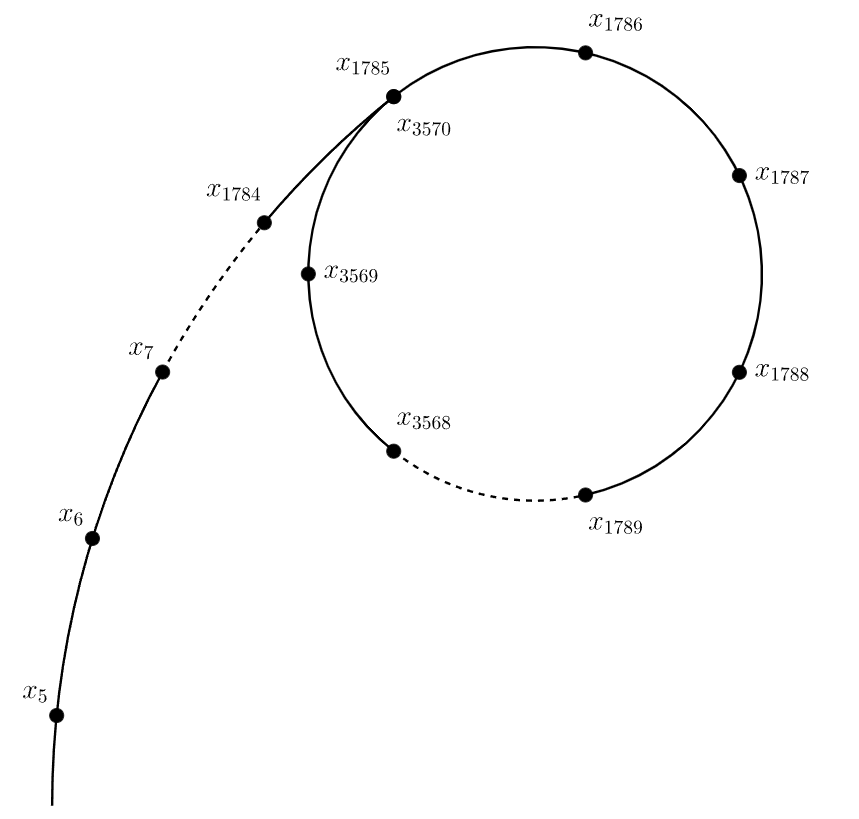
\includegraphics[width=0.6\textwidth]{contents/0x30 数学/figures/0x34 rho 形图.png}
\end{center}

我们发现，\textbf{若 $x \equiv y \pmod p$，必有 $f(x) \equiv f(y) \pmod p$}。由此可得\textbf{在模 $p$ 的环上，只要某个相距 $d$ 步的点对满足条件，则所有相距 $d$ 步的点对均满足条件}。所以我们每次最好要检查不同的距离。

\textbf{Brent 倍增迭代}：初始有两个点 $a, b$，在第 $k$ 轮，$a$ 原地不动，$b$ 不断地向前共计 $2^k$ 步，最后再让 $a$ 直接跳到 $b$ 的位置。$b$ 的每一步移动，我们都计算 $d = \gcd(|a - b|, n)$，当第一次出现 $d > 1$ 时

\begin{itemize}
\item 若 $1 < d < n$，则我们已经找到了一个非平凡因数，直接返回 $d$。
\item 若 $d = n$，则说明我们已经完整地跑完了一个环，继续在环上跑也没有意义。\newline{}
此时我们应该换个映射，或者换一个初始值继续做。
\end{itemize}

\textbf{进一步，我们想要降低求解 $\gcd$ 的次数}。注意到，如果 $\gcd(a, n) > 1$，则对于任意正整数 $b$ 均有 $\gcd(ab \bmod n, n) = \gcd(ab, n) > 1$。

也就是说，如果 $\gcd\left(\prod |x_i - x_j| \bmod n, n\right) > 1$，那么其中必有一对 $x_i, x_j$ 满足 $\gcd(|x_i - x_j|, n) > 1$。

于是我们每 $k$ 对 $a, b$ 就计算一次 $\gcd$。时间复杂度 $\mathcal{O}(\sqrt{p} + k^{-1}\sqrt{p} \log n)$，当 $k$ 与 $\log n$ 大致相等时，\textbf{可以得到 $\mathcal{O}(\sqrt{p})$ 的理论复杂度}。具体实现中，一般取 $k = 128$。

\Highlight{Pollard-Rho 质因数分解}：如果要对 $n$ 进行质因数分解，先使用 Miller-Rabin 判断 $n$ 是否是质数，若 $n$ 为合数，则使用 Pollard-Rho 找出 $n$ 的一个非平凡因数 $d$，得到两个规模分别为 $d$ 和 $\frac{n}{d}$ 的两个子问题，递归进行求解。

\InputCode{cpp}{contents/0x30 数学/code/0x34 素性测试与质因数分解（Miller-Rabin + Pollard-Rho）.cpp}

\section{0x34\ 数学\ 初等数论-约数}
\label{sec:0x34b}

\subsection{约数}

\Highlight{整除}：设 $d, n \in \mathbb{Z}$ 且 $d \neq 0$，如果 $\exists q \in \mathbb{Z}$ 使得 $qd = n$，那么称 $d$ 整除 $n$（记作 $d \mid n$）。

\Highlight{整除的简单性质}：

\begin{itemize}
\item $a \mid b \land b \mid c \Longrightarrow a\mid c$。
\item $a \mid b \land a \mid c \Longrightarrow \forall x, y \in \mathbb{Z}, a \mid (xb + yc)$。
\item 设 $m \neq 0$，则 $a \mid b \Longrightarrow ma \mid mb$。
\item 设 $\gcd(a, m) = 1$，则 $a \mid mb \Longrightarrow a\mid b$。
\end{itemize}

\Highlight{约数个数}：

\begin{itemize}
\item $n$ 的约数个数必定不超过 $2\sqrt{n}$。实际上很难到达该上界，可以简单认为在 $10^6 \sim 10^{18}$ 范围内为 $\mathcal{O}(\sqrt[3]{n})$ 级别。
\item $1\sim n$ 的约数个数总和为 $\mathcal{O}(n \log n)$ 级别。
\end{itemize}

\subsection{最大公约数与最小公倍数}

\Highlight{最大公约数}：最大的公共约数（\textbf{G}reatest \textbf{C}ommon \textbf{D}ivisor，简写 GCD）。

\Highlight{最小公倍数}：最小的公共倍数（\textbf{L}east \textbf{C}ommon \textbf{M}ultiple，简写 LCM）。

\Highlight{\textbf{唯一分解角度下的 gcd 与 lcm}}：设 $a = p_1^{c_1}p_2^{c_2}\dots$，$b = p_1^{d_1}p_2^{d_2} \dots$，则有
\[
\begin{gathered}
\gcd(a, b) = p_1^{\min(c_1, d_1)}p_2^{\min(c_2, d_2)} \dots \\
\mathrm{lcm}(a, b) = p_1^{\max(c_1, d_1)}p_2^{\max(c_2, d_2)} \dots
\end{gathered}
\]
在唯一分解角度下，\textbf{gcd 相当于是对每个指数取 min，lcm 相当于是对每个指数取 max}。

\Highlight{gcd 的简单性质}：

\begin{itemize}
\item $\gcd(a_1, \dots, a_n) = \gcd(|a_1|, \dots, |a_n|)$。
\item $\gcd(a, 0) = \gcd(a, a) = |a|$。
\item $\gcd(bq + r, b) = \gcd(r, b)$。
\item 设 $\gcd(a, m) = 1$，则 $\gcd(a, mb) = \gcd(a, b)$。
\item $\gcd(ma_1, \dots, ma_n) = |m| \gcd(a_1, \dots, a_n)$。
\end{itemize}

\Highlight{lcm 的简单性质}：

\begin{itemize}
\item $\mathrm{lcm}(a_1, \dots, a_n) = \mathrm{lcm}(|a_1|, \dots, |a_n|)$。
\item $\mathrm{lcm}(a, 1) = \mathrm{lcm}(a, a) = |a|$。
\item $\mathrm{lcm}(ma_1, \dots, ma_n) = |m| \operatorname{lcm}(a_1, \dots, a_n)$。
\end{itemize}

\subsubsection{gcd 和 lcm 的常见恒等式}

\Highlight{gcd-lcm 恒等式}：
\[
\gcd(a, b) \operatorname{lcm}(a, b) = ab
\]
请注意！\textbf{该式子扩展到三元以上几乎不成立！}

事实上当 $n \geq 3$ 时，$\gcd(a_1, \dots, a_n) \operatorname{lcm}(a_1, \dots, a_n) = a_1\dots a_n$ 当且仅当 $a_1, \dots, a_n$ 两两互质。

\Highlight{gcd 和 lcm 的结合律}：
\[
\begin{gathered}
\gcd(a, b, c) = \gcd(\gcd(a, b), c) \\
\mathrm{lcm}(a, b, c) = \mathrm{lcm}(\mathrm{lcm}(a, b), c)
\end{gathered}
\]
该式子扩展到任意多元仍然成立。

于是可以使用恒等式 $\mathrm{lcm}(a, b) = \frac{ab}{\gcd(a, b)}$，用来求解 $\mathrm{lcm}(a, b, c)$，以及 $\mathrm{lcm}(a_1, \dots, a_n)$。

\Highlight{gcd 对乘法的分配律}：
\[
\gcd(a, bc) = \gcd(a, b) \gcd\left(\frac{a}{\gcd(a, b)}, c\right)
\]
根据对乘法的分配律计算 $\gcd(a, b_1\dots b_n)$。每次处理 $b_i$ 时，计算 $t = \gcd(a, b_i)$，然后将 $a$ 除以 $t$（相当于是将已计算的质因数贡献去掉），答案乘以 $t$。

\Highlight{gcd 的差分律}：
\[
\gcd(a_1, a_2, \dots, a_n) = \gcd(a_1, a_2 - a_1, \dots, a_n - a_{n - 1})
\]
通过差分律，我们可以维护差分数组的 gcd，以实现 “区间加” 与 “区间 gcd”。

\Highlight{斐波那契数列 gcd 恒等式}：
\[
\gcd(\mathrm{Fib}_n, \mathrm{Fib}_m) = \mathrm{Fib}_{\gcd(n, m)}
\]
\Highlight{幂差 gcd 恒等式}：\textbf{不妨设 $a \geq b$，当 $\gcd(a, b) = 1$ 时}，有
\[
\gcd(a^n - b^n, a^m - b^m) = a^{\gcd(n, m)} - b^{\gcd(n, m)}
\]
简单推导：

\textbf{右边整除左边}：可以证明 $x - y \mid x^k - y^k$。

\begin{quoteblock}
$k$ 次方差公式：$x^k - y^k = (x - y)(x^{k - 1} + x^{k - 2}y + \dots + xy^{k - 2} + y^{k - 1})$。
\end{quoteblock}

对于 $n, m$ 的公约数 $d$ 来说，可以证得 $a^d - b^d \mid a^n - b^n$ 与 $a^d - b^d \mid a^m - b^m$。

于是 $a^d - b^d \mid \gcd(a^n - b^n, a^m - b^m)$。所以
\[
a^{\gcd(n, m)} - b^{\gcd(n, m)} \mid \gcd(a^n - b^n, a^m - b^m)
\]
\textbf{左边整除右边}：

\begin{quoteblock}
“降幂引理”：不妨设 $r \geq s$，当 $\gcd(a, b) = 1$ 时，有
\[
\gcd(a^r - b^r, a^s - b^s) \mid a^{r - s} - b^{r - s}
\]

证明：设 $d$ 为 $a^r - b^r, a^s - b^s$ 的公约数。

因为 $(a^r - b^r) - a^{r - s}(a^s - b^s) = b^s(a^{r - s} - b^{r - s})$，可以证得 $d \mid b^s(a^{r - s} - b^{r - s})$；同理可得 $d \mid a^s(a^{r - s} - b^{r - s})$。

又由于 $\gcd(a, b) = 1$，于是 $d \mid a^{r - s} - b^{r - s}$，“降幂引理” 得证。
\end{quoteblock}

对 $\gcd(a^n - b^n, a^m - b^m)$ 反复应用 “降幂引理”，过程等价于辗转相除法。所以
\[
\gcd(a^n - b^n, a^m - b^m) \mid a^{\gcd(n, m)} - b^{\gcd(n, m)}
\]

\subsection{最大公约数常见求法}

已有的轮子：\texttt{std::gcd(a, b)}。

\subsubsection{求法 1：辗转相除法}

（也称之为欧几里得算法）

对于 $\forall a, b \in \mathbb{N}$ 且 $b \neq 0$，有
\[
\gcd(a, b) = \gcd(b, a \bmod b)
\]

\begin{itemize}
\item 当 $a < b$ 时，一次迭代后就会转化为 $a \geq b$。
\item 当 $a \geq b$ 时，由于 $a \bmod b \leq \frac{a}{2}$，这样的迭代不超过 $\log_2 a$ 次。
\end{itemize}

时间复杂度 $\mathcal{O}(\log \max(a, b))$。

使用辗转相除法求解斐波那契数列相邻两项的 gcd，会让该算法达到最坏复杂度。

\begin{minted}{cpp}
// 辗转相除法
int gcd(int a, int b) {
    return b == 0 ? a : gcd(b, a % b);
}
\end{minted}

\subsubsection{求法 2：更相减损术}

对于 $\forall a, b \in \mathbb{N}$，不妨设 $a\geq b$，有
\[
\begin{gathered}
\gcd(a, b) = \gcd(a, a - b) = \gcd(b, a - b) \\
\gcd(2a, 2b) = 2\gcd(a, b)
\end{gathered}
\]

\begin{itemize}
\item 当 $a = b$ 时，$\gcd(a, b) = a$。
\item “两个偶数”：$\gcd(a, b) = 2\gcd(\frac{a}{2}, \frac{b}{2})$。
\item “一奇一偶”：不妨设 $a$ 为偶数，$\gcd(a, b) = \gcd(\frac{a}{2}, b)$。
\item “两个奇数”：不妨设 $a \geq b$，$\gcd(a, b) = \gcd(a - b, b)$。
\end{itemize}

当至少有一个偶数的时候，每次迭代至少会将 $a, b$ 之一减半。而两个奇数相减会得到偶数。

时间复杂度 $\mathcal{O}(\log \max(a, b))$。

更相减损术常用于计算高精度 gcd（因为“高精度取模”复杂度较高，“高精度减法”以及“高精除低精”复杂度较低）。

\InputCode{cpp}{contents/0x30 数学/code/0x34 gcd（更相减损术）.cpp}

\subsubsection{求法 3：递推}

初值 $\gcd(i, 0) = \gcd(0, i) = i$，递推式 $\gcd(i, j) = \gcd(i - j, j)$。

时间复杂度：预处理 $\mathcal{O}(n^2)$，查询 $\mathcal{O}(1)$。

\begin{minted}{cpp}
for (int i = 0; i <= n; i ++) {
    g[i][0] = g[0][i] = i;
    for (int j = 1; j <= i; j ++) {
        g[i][j] = g[j][i] = g[i - j][j];
    }
}
\end{minted}

\subsubsection{求法 4：基于值域预处理的快速 gcd}

\textbf{引理}：对于任意正整数 $n$，一定可以被拆分成三个正整数 $a, b, c$ ($a \leq b \leq c$) 的乘积，其中 $a, b\leq \sqrt{n}$，且 $c \leq \sqrt{n}$ 与 $c \in \mathbb{P}$ 至少有一个成立。

\textbf{证明 1}：假设 $c > \sqrt{n}$ 且 $c \notin \mathbb{P}$。因为 $c > \sqrt{n}$ 且 $abc = n$，所以 $ab \leq \sqrt{n}$。由于 $c$ 不是质数，设 $c = xy$，显然 $x, y$ 不可能同时 $>\sqrt{n}$，不妨设 $x \leq y$，则必有 $x \leq \sqrt{n}$。此时 $n$ 可以被拆分成 $x, ab, y$ 的乘积。不断对 $y$ 进行相同的讨论。

由于数值不断递减，迭代到最后 $c \leq \sqrt{n}$ 与 $c \in \mathbb{P}$ 至少有一个成立。

\textbf{证明 2}：考虑归纳。当 $n = 1$ 时显然成立。当 $n > 1$ 时，设 $p$ 为 $n$ 的最小质因数，设 $a', b', c'$ ($a' \leq b' \leq c'$) 为 $\frac{n}{p}$ 的一组合法拆分。

\begin{itemize}
\item 当 $p \leq \sqrt[4]{n}$ 时。由于 $a' \leq \sqrt[3]{\frac{n}{p}}$，所以 $pa' \leq \sqrt[3]{np^2} \leq \sqrt{n}$。此时 $pa', b', c'$ 为一组合法拆分。
\item 当 $p > \sqrt[4]{n}$ 时。假设 $a' \geq p$，则 $n = pa'b'c' \geq p^4 > n$ 矛盾，故 $a' < p$。由于 $p$ 为 $n$ 的最小质因数，所以 $a' = 1$。此时 $p, b', c'$ 为一组合法拆分。
\end{itemize}

\Separator{}

预处理：通过线性筛得出 $1 \sim n$ 所有数的最小质因数。然后根据证明 2，递推得出 $1 \sim n$ 所有数的合法拆分。对于 $i > 1$，设 $p$ 为 $i$ 的最小质因数，\textbf{将 $\frac{i}{p}$ 的合法拆分中的最小数乘以 $p$ 即可得到 $i$ 的合法拆分}。最后预处理出所有 $0 \leq x, y \leq \sqrt{n}$ 的 $\gcd(x, y)$。

查询：当询问 $\gcd(p, q)$ 时，根据 gcd 对乘法的分配律，依次考虑 $q$ 的合法拆分 $a, b, c$，设当前考虑到的数为 $x$。

\begin{itemize}
\item 计算 $t = \gcd(p, x)$，具体地：
  \begin{itemize}
  \item 若 $x$ 为合数（此时 $x \leq \sqrt{n}$），则 $\gcd(p, x) = \gcd(x, p \bmod x)$。使用预处理的 gcd 值回答即可。
  \item 若 $x$ 为质数，则当且仅当 $p$ 为 $x$ 的倍数时 $\gcd(p, x) = x$，否则 $\gcd(p, x) = 1$。
  \end{itemize}
\item 然后将 $p$ 除以 $t$，答案乘以 $t$。
\end{itemize}

时间复杂度：预处理 $\mathcal{O}(n)$，查询 $\mathcal{O}(1)$。

\InputCode{cpp}{contents/0x30 数学/code/0x34 gcd（基于值域预处理的快速 gcd）.cpp}

\subsection{类欧几里得算法}

\Highlight{类欧几里得算法}：用来解决一类形如 $\left\lfloor \frac{ai + b}{c} \right\rfloor$ 结构的求和问题。

基本模型为
\[
f(a, b, c, n) = \sum_{i = 0}^n \left\lfloor \frac{ai + b}{c} \right\rfloor
\]
首先，可以转化为 $0 \leq a, b < c$ 的情况
\[
\begin{aligned}
f(a, b, c, n) & = \sum_{i = 0}^n \left\lfloor \frac{ai + b}{c} \right\rfloor \\
& = \sum_{i = 0}^n \left\lfloor \frac{\left(\left\lfloor \frac{a}{c} \right\rfloor c + (a \bmod c) \right)i + \left(\left\lfloor \frac{b}{c} \right\rfloor c + (b \bmod c)\right)}{c} \right\rfloor \\
& = \sum_{i = 0}^n \left( \left\lfloor \frac{a}{c} \right\rfloor i + \left\lfloor \frac{b}{c} \right\rfloor + \left\lfloor \frac{(a \bmod c) i + (b \bmod c)}{c} \right\rfloor \right) \\
& = \frac{n(n + 1)}{2} \left\lfloor \frac{a}{c} \right\rfloor + (n + 1)\left\lfloor \frac{b}{c} \right\rfloor + f(a \bmod c, b \bmod c, c, n)
\end{aligned}
\]
然后，令 $m = \left\lfloor \frac{an + b}{c} \right\rfloor$
\[
\begin{aligned}
f(a, b, c, n) & = \sum_{i = 0}^n \left\lfloor \frac{ai + b}{c} \right\rfloor \\
& = \sum_{i = 0}^n \sum_{j = 0}^{m - 1} \left[ j < \left\lfloor \frac{ai + b}{c} \right\rfloor \right] \\
& = \sum_{i = 0}^n \sum_{j = 0}^{m - 1} \left[ j + 1 \leq \frac{ai + b}{c} \right] \\
& = \sum_{i = 0}^n \sum_{j = 0}^{m - 1} \left[ cj + c - b - 1 < ai \right] \\
& = \sum_{j = 0}^{m - 1} \sum_{i = 0}^n \left[ \left\lfloor \frac{cj + c - b - 1}{a} \right\rfloor < i \right] \\
& = \sum_{j = 0}^{m - 1} \left( n - \left\lfloor \frac{cj + c - b - 1}{a} \right\rfloor \right) \\
& = nm - f(c, c - b - 1, a, m - 1)
\end{aligned}
\]

结合这两步操作，二元组 $(a, c) \to (c, a \bmod c)$，相当于对 $(a, c)$ 进行辗转相除法，故称之为类欧几里得算法。

时间复杂度 $\mathcal{O}(\log \min(a, c))$。

\InputCode{cpp}{contents/0x30 数学/code/0x34 类欧几里得算法.cpp}

\section{0x34\ 数学\ 初等数论-取整}
\label{sec:0x34c}

\subsection{取整}

\Highlight{向下取整}：$\lfloor x \rfloor$，表示不超过 $x$ 的最大整数（floor）。

\Highlight{向上取整}：$\lceil x \rceil$，表示不小于 $x$ 的最小整数（ceiling）。

注意：C++ 中的整数除法结果\textbf{向零取整}，取模结果\textbf{与被除数同号}，与数学中的取整有较大区别。

\Highlight{取整的简单性质}：

\begin{itemize}
\item $x - 1 < \lfloor x \rfloor \leq x$，$x \leq \lceil x \rceil < x + 1$。
\item $\lfloor -x \rfloor = - \lceil x \rceil$，$\lceil -x \rceil = - \lfloor x \rfloor$。
\end{itemize}

\subsubsection{取整的常见恒等式}

\Highlight{上下取整的相互转化}：$n, m \in \mathbb{Z}$，$m > 0$
\[
\begin{gathered}
\left\lceil \frac{n}{m} \right\rceil = \left\lfloor \frac{n + m - 1}{m} \right\rfloor = \left\lfloor \frac{n - 1}{m} \right\rfloor + 1 \\
\left\lfloor \frac{n}{m} \right\rfloor = \left\lceil \frac{n - m + 1}{m} \right\rceil = \left\lceil \frac{n + 1}{m} \right\rceil - 1
\end{gathered}
\]
\Highlight{上下取整的嵌套恒等式}：$a, b, c \in \mathbb{N}_+$
\[
\begin{gathered}
\left\lfloor \frac{ \left\lfloor \frac{a}{b} \right\rfloor }{c} \right\rfloor = \left\lfloor \frac{a}{bc} \right\rfloor \\
\left\lceil \frac{ \left\lceil \frac{a}{b} \right\rceil }{c} \right\rceil = \left\lceil \frac{a}{bc} \right\rceil
\end{gathered}
\]

\Highlight{上下取整对加法的恒等式}：$A, B, C, D \in \mathbb{N}_+$
\[
\begin{gathered}
\left\lfloor \frac{ \left\lfloor \frac{A}{B} \right\rfloor + C }{D} \right\rfloor = \left\lfloor \frac{A + BC}{BD} \right\rfloor \\
\left\lceil \frac{ \left\lceil \frac{A}{B} \right\rceil + C }{D} \right\rceil = \left\lceil \frac{A + BC}{BD} \right\rceil
\end{gathered}
\]

\subsection{数论分块}

也称之为整除分块。

\subsubsection{下取整数论分块}

给出一个正整数 $n$，记 $D_n$ 表示 $\left\lfloor \frac{n}{d} \right\rfloor$ 所有可能的取值构成的集合，即 $D_n = \{ \left\lfloor \frac{n}{d} \right\rfloor \mid 1 \leq d \leq n \}$。

\textbf{性质 1}：$\left\lfloor \frac{n}{d} \right\rfloor$ 的取值不超过 $2\sqrt{n}$ 种，即 $|D_n| \leq 2\sqrt{n}$。

简单推导：

\begin{itemize}
\item 当 $d \leq \sqrt{n}$ 时，因为 $d$ 的取值不超过 $\sqrt{n}$ 种，所以此时 $\left\lfloor \frac{n}{d} \right\rfloor$ 的取值不超过 $\sqrt{n}$ 种。
\item 当 $d > \sqrt{n}$ 时，因为 $\left\lfloor \frac{n}{d} \right\rfloor \leq \sqrt{n}$，所以此时 $\left\lfloor \frac{n}{d} \right\rfloor$ 的取值不超过 $\sqrt{n}$ 种。
\end{itemize}

\textbf{性质 2}：若 $m \in D_n$，则 $D_m \subseteq D_n$。

简单推导：设 $m = \left\lfloor \frac{n}{k} \right\rfloor$，此时对于任意 $d \in \mathbb{N}_+$
\[
\left\lfloor \frac{m}{d} \right\rfloor = \left\lfloor \frac{\left\lfloor \frac{n}{k} \right\rfloor}{d} \right\rfloor = \left\lfloor \frac{n}{kd} \right\rfloor \in D_n
\]
这意味着，\textbf{如果我们想要递归地应用数论分块（类似杜教筛）}，在计算过程中涉及到的取值集合均为 $D_n$。

\Highlight{下取整数论分块}：快速地划分出 $\left\lfloor \frac{n}{d} \right\rfloor$ 取值相同的所有区间。

由于函数 $\frac{n}{x}$ 在区间 $(0, +\infty)$ 上单调递减，所以 $\left\lfloor \frac{n}{x} \right\rfloor$ 取值相同的所有自变量 $x$ \textbf{构成一段连续的区间}。并且由上述分析，这样的区间不超过 $2\sqrt{n}$ 个。

对于任意 $i$ ($1 \leq i \leq n$)，需要找到一个最大的 $j$ ($i \leq j \leq n$) 满足 $\left\lfloor \frac{n}{i} \right\rfloor = \left\lfloor \frac{n}{j} \right\rfloor$。由不等式 $\left\lfloor \frac{n}{i} \right\rfloor \leq \frac{n}{j}$ 可得 $\boldsymbol{j = \left\lfloor \frac{n}{\left\lfloor \frac{n}{i} \right\rfloor} \right\rfloor}$。

根据该公式，我们就可以根据区间的左端点计算出右端点。于是依次遍历所有区间即可。

\begin{minted}{cpp}
// h 表示 x 的上界
for (int x = 1, nx; x <= h; x = nx + 1) {
    nx = h;
    if (x <= n) {
        chmin(nx, n / (n / x));
    }
    // 区间 [x, nx] 内：下取整的值均为 n/x
}
\end{minted}

\begin{quoteblock}
By the way：数论分块套数论分块的时间复杂度为 $\mathcal{O}(n^{\frac{3}{4}})$。
\end{quoteblock}

\subsubsection{上取整数论分块}

\Highlight{上取整数论分块}：快速地找出 $\lceil \frac{n}{d} \rceil$ 取值相同的所有区间。

由恒等式 $\left\lceil \frac{n}{m} \right\rceil = \left\lfloor \frac{n - 1}{m} \right\rfloor + 1$ 可知，$n$ 的上取整数论分块与 $n - 1$ 的下取整数论分块，分出的区间是一样的。

于是套用 $n - 1$ 的下取整数论分块即可，\textbf{注意 $d \geq n$ 的特殊情况}。

\begin{minted}{cpp}
// h 表示 x 的上界
for (int x = 1, nx; x <= h; x = nx + 1) {
    nx = h;
    if (x < n) {
        chmin(nx, (n - 1) / ((n - 1) / x));
    }
    // 区间 [x, nx] 内：上取整的值均为 (n-1)/x+1
}
\end{minted}

\subsubsection{多维数论分块}

\Highlight{二维数论分块}：快速地找出 $\left\lfloor \frac{n}{d} \right\rfloor, \left\lfloor \frac{m}{d} \right\rfloor$ 取值均相同的所有区间。

显然，这样的区间不超过 $2\sqrt{n} + 2\sqrt{m}$ 个。

对于任意 $i$，需要找到一个最大的 $j$ 满足 $\left\lfloor \frac{n}{i} \right\rfloor = \left\lfloor \frac{n}{j} \right\rfloor, \left\lfloor \frac{m}{i} \right\rfloor = \left\lfloor \frac{m}{j} \right\rfloor$。则有 $\boldsymbol{j = \min\left\{ \left\lfloor \frac{n}{ \left\lfloor \frac{n}{i} \right\rfloor } \right\rfloor, \left\lfloor \frac{m}{ \left\lfloor \frac{m}{i} \right\rfloor } \right\rfloor \right\}}$。

扩展到多维也是一样。

\begin{minted}{cpp}
// h 表示 x 的上界
for (int x = 1, nx; x <= h; x = nx + 1) {
    nx = h;
    if (x <= n) {
        chmin(nx, n / (n / x));
    }
    if (x <= m) {
        chmin(nx, m / (m / x));
    }
    // 区间 [x, nx] 内：n, m 对 x 下取整的值分别为 n/x, m/x
}
\end{minted}

\subsection{积性函数与狄利克雷卷积}

\Highlight{积性函数}：若数论函数 $f(n)$，对于\textbf{任意互质}正整数 $x, y$，都有 $f(xy) = f(x)f(y)$，则称 $f(n)$ 为积性函数。

\Highlight{完全积性函数}：若数论函数 $f(n)$，对于\textbf{任意}正整数 $x, y$，都有 $f(xy) = f(x)f(y)$，则称 $f(n)$ 为完全积性函数。

\Highlight{积性函数的简单性质}：

\begin{itemize}
\item 对于任意积性函数 $f(x)$（除了恒为 $0$ 的函数），有 $f(1) = 1$。
\item 对于任意积性函数 $f(x), g(x)$，\textbf{以下的函数仍为积性函数}
\[
\begin{gathered}
f(x^p) \\
f^p(x) \\
f(x)g(x) \\
\sum_{d \mid x} f(d)g\left( \frac{x}{d} \right)
\end{gathered}
\]

\item 对于任意积性函数 $f(x)$，将 $x$ 唯一分解成 $x = p_1^{c_1}p_2^{c_2}\dots p_t^{c_t}$，有 $f(x) = \prod_{i = 1}^t f(p_i^{c_i})$。
\end{itemize}

\subsubsection{常见积性函数（及性质）}

\paragraph{单位函数（完全积性）}
\[
\epsilon(n) = [n = 1]
\]

\paragraph{恒等函数（完全积性）}
\[
\mathrm{ID}_k(n) = n^k
\]

当 $k = 1$ 时，亦可简写为 $\mathrm{ID}(n) = n$。

\paragraph{常数函数（完全积性）}
\[
1(n) = 1
\]

\paragraph{约数函数（积性）}

\Highlight{约数函数}：
\[
\sigma_k(n) = \sum_{d \mid n} d^k
\]

当 $k = 0$ 时，$\sigma_0(n)$ 表示 $n$ 的约数个数函数。

\Highlight{约数个数函数的前缀和}：
\[
\sum_{i = 1}^n \sigma_0(i) = \sum_{i = 1}^n \left\lfloor \frac{n}{i} \right\rfloor
\]
\Highlight{乘积的约数个数函数}：
\[
\begin{gathered}
\sigma_0(ij) = \sum_{x \mid i} \sum_{y \mid j} [\gcd(x, y) = 1] \\
\sigma_0(ijk) = \sum_{a \mid i} \sum_{b \mid j} \sum_{c \mid k} [\gcd(a, b) = \gcd(b, c) = \gcd(a, c) = 1]
\end{gathered}
\]
简单推导（仅证二维）：从唯一分解的角度，对每个质因子 $p$ 单独考虑。$p$ 在 $(x, y)$ 中的出现情况数，为 $i, j$ 中质因子 $p$ 的个数之和再加 $1$。将所有质因子 $p$ 的贡献相乘，这正是 $\sigma_0(ij)$ 的表达式。

可以扩展至更多维。

\paragraph{欧拉函数（积性）}

\Highlight{欧拉函数}：$\varphi(n)$，表示 $1 \sim n$ 中与 $n$ 互质的数的个数。将 $n$ 唯一分解成 $n = p_1^{c_1}p_2^{c_2}\dots p_t^{c_t}$，则欧拉函数为
\[
\varphi(n) = n \prod_{i = 1}^t (1 - \frac{1}{p_i})
\]

\Highlight{乘积的欧拉函数}：
\[
\varphi(ij) = \frac{\varphi(i) \varphi(j) \gcd(i, j)}{\varphi(\gcd(i, j))}
\]
简单推导：设 $P(n)$ 表示 $n$ 的质因数集合，则有 $P(ij) = P(i) \cup P(j)$ 与 $P(\gcd(i, j)) = P(i) \cap P(j)$。

由容斥原理得
\[
\prod_{p \mid ij} \left(1 - \frac{1}{p}\right) = \frac{\prod_{p \mid i} \left(1 - \frac{1}{p}\right) \prod_{p \mid j} \left(1 - \frac{1}{p}\right)}{\prod_{p \mid \gcd(i, j)} \left(1 - \frac{1}{p}\right)}
\iff
\frac{\varphi(ij)}{ij} = \frac{ \frac{\varphi(i)}{i} \frac{\varphi(j)}{j} }{\frac{\varphi(\gcd(i, j))}{\gcd(i, j)}}
\]

\paragraph{莫比乌斯函数（积性）}

\Highlight{莫比乌斯函数}：$\mu(n)$，将 $n$ 唯一分解成 $n = p_1^{c_1}p_2^{c_2}\dots p_t^{c_t}$，则莫比乌斯函数有如下的定义
\[
\mu(n) = \begin{cases}
(-1)^t & \forall i\in[1, t], c_i = 1 \\
0 & \exists i\in[1, t], c_i > 1
\end{cases}
\]
特别地，$\mu(1) = 1$。

\Highlight{莫比乌斯函数的平方}：
\[
\mu^2(n) = \sum_{d^2 \mid n} \mu(d)
\]
简单推导：记 $m = \prod p_i^{\left\lfloor c_i / 2 \right\rfloor}$，则 $d^2 \mid n \iff d \mid m$，由 $\sum_{d \mid m}\mu(d) = [m = 1]$ 可证。

\subsubsection{线性筛筛积性函数}

对于积性函数 $f(x)$，若\textbf{质数幂的函数值 $f(p^c)$ 便于求出}。则 $f(x)$ 的前 $n$ 项函数值可以通过线性筛得出。

具体地，记 $\mathrm{low}_i$ 表示：设 $i$ 的最小质因子为 $p_1$，其次数为 $c_1$，则 $\mathrm{low}_i = p_1^{c_1}$。

在线性筛的过程中，额外进行如下的维护

\begin{itemize}
\item 维护 $\mathrm{low}_i$ 数组。
\item 每当筛出一个质数 $p$，就将 $f(p), f(p^2), \dots, f(p^c)$ 全都求出来。
\item 其余满足 $i \neq\mathrm{low}_i$ 的 $i$，使用递推式 $f(i) = f(\mathrm{low}_i) \times f\left(\frac{i}{\mathrm{low}_i}\right)$ 计算函数值。
\end{itemize}

\InputCode{cpp}{contents/0x30 数学/code/0x34 线性筛筛积性函数.cpp}

\subsubsection{狄利克雷卷积}

\Highlight{狄利克雷卷积}：对于两个数论函数 $f, g$，定义 $f, g$ 的狄利克雷卷积为
\[
(f \ast g)(x) = \sum_{d \mid x} f(d)g\left( \frac{x}{d} \right)
\]
\Highlight{狄利克雷卷积的简单性质}：

\begin{itemize}
\item 交换律：$f \ast g = g \ast f$。
\item 结合律：$(f \ast g) \ast h = f \ast (g \ast h)$。
\item 分配律：$f \ast (g + h) = f \ast g + f \ast h$。
\item 单位元：$f \ast \epsilon = \epsilon \ast f = f$，因此 $\epsilon$ 又被称为狄利克雷卷积的单位元。
\end{itemize}

\subsubsection{常见狄利克雷卷积式}

\paragraph{式 1}
\[
\boldsymbol{\epsilon = \mu \ast 1 \iff \sum_{d \mid n} \mu(d) = [n = 1]}
\]

简单推导：由积性函数的简单性质可知，关于 $n$ 的函数 $f(n) = \sum_{d \mid n} \mu(d)$ 为积性函数。

\begin{itemize}
\item 当 $n = 1$ 时，等式成立。
\item 当 $n > 1$ 时，将 $n$ 唯一分解成 $n = p_1^{c_1}p_2^{c_2}\dots p_t^{c_t}$，则有
\[
\begin{aligned}
f(n) & = \prod_{i = 1}^t f(p_i^{c_i}) \\
& = \prod_{i = 1}^t \left( \sum_{j = 0}^{c_i} \mu(p_i^j) \right) \\
& = \prod_{i = 1}^t \left( \mu(1) + \mu(p_i) \right) \\
& = 0
\end{aligned}
\]
\end{itemize}

综上，$\sum_{d \mid n} \mu(d) = [n = 1]$。

\paragraph{式 2}
\[
\boldsymbol{\mathrm{ID} = \varphi \ast 1 \iff \sum_{d \mid n} \varphi(d) = n}
\]

简单推导：由积性函数的简单性质可知，关于 $n$ 的函数 $f(n) = \sum_{d \mid n} \varphi(d)$ 为积性函数。

\begin{itemize}
\item 当 $n = 1$ 时，等式成立。
\item 当 $n > 1$ 时，将 $n$ 唯一分解成 $n = p_1^{c_1}p_2^{c_2}\dots p_t^{c_t}$，则有
\[
\begin{aligned}
f(n) & = \prod_{i = 1}^t f(p_i^{c_i}) \\
& = \prod_{i = 1}^t \left( \sum_{j = 0}^{c_i} \varphi(p_i^j) \right) \\
& = \prod_{i = 1}^t \left( 1 + \sum_{j = 1}^{c_i}(p_i^{j} - p_i^{j - 1}) \right) \\
& = \prod_{i = 1}^t p_i^{c_i} \\
& = n
\end{aligned}
\]
\end{itemize}

综上，$\sum_{d \mid n} \varphi(d) = n$。

\paragraph{式 3}
\[
\boldsymbol{\varphi = \mu \ast \mathrm{ID} \iff \varphi(n) = \sum_{d \mid n} d\mu\left( \frac{n}{d} \right)}
\]

简单推导：
\[
\begin{aligned}
\varphi \ast 1 = \mathrm{ID} & \Longrightarrow \varphi \ast 1 \ast \mu = \mathrm{ID} \ast \mu \\
& \Longrightarrow \varphi \ast \epsilon = \mathrm{ID} \ast \mu \\
& \Longrightarrow \varphi = \mathrm{ID} \ast \mu
\end{aligned}
\]

\subsection{杜教筛}

\Highlight{杜教筛}：用于 $\mathcal{O}(n^{\frac{2}{3}})$ 时间内，求解一类数论函数 $f(x)$ 的前缀和。

\begin{itemize}
\item $f(x)$ 为积性函数。
\item 存在辅助函数 $g(x)$，满足函数 $f \ast g$ 与 $g$ 的前缀和便于求出。
\end{itemize}

\Separator{}

记 $S(n) = \sum_{i = 1}^n f(i)$。取杜教筛中的辅助函数 $g(x)$，则有
\[
\begin{aligned}
\sum_{i = 1}^n (f \ast g)(i) & = \sum_{i = 1}^n \sum_{d \mid i} g(d)f\left( \frac{i}{d} \right) \\
& = \sum_{i = 1}^n g(i) \sum_{j = 1}^{\left\lfloor \frac{n}{i} \right\rfloor} f(j) \\
& = \sum_{i = 1}^n g(i) S\left( \left\lfloor \frac{n}{i} \right\rfloor \right)
\end{aligned}
\]
移项得
\[
g(1)S(n) = \sum_{i = 1}^n (f \ast g)(i) - \sum_{i = 2}^n g(i)S\left( \left\lfloor \frac{n}{i} \right\rfloor \right)
\]
此时得到了一个 $S(n)$ 关于 $S\left( \left\lfloor \frac{n}{i} \right\rfloor \right)$ 的递推式。\textbf{若函数 $f \ast g$ 与 $g$ 的前缀和便于求出，就可以使用数论分块处理该式}。因此找到一个合适的辅助函数 $g$ 是杜教筛的关键。

\Highlight{杜教筛的时间复杂度分析}：

由数论分块的性质，对于 $m \in D_n$，有 $D_m \subseteq D_n$。于是我们\textbf{需要使用记忆化保证杜教筛的复杂度}，使用记忆化以后，只需要对所有的 $k \in D_n$ 计算一次 $S(k)$ 即可。

假设函数 $f \ast g$ 与 $g$ 的前缀和均可 $\mathcal{O}(1)$ 求出，设计算 $S(n)$ 的时间复杂度为 $T(n)$，则有
\[
\begin{aligned}
T(n) & = \sum\limits_{k \in D_n} T(k) \\
& = \mathcal{O}(\sqrt{n}) + \sum_{i = 1}^{\sqrt{n}}\mathcal{O}(\sqrt{i}) + \sum_{i = 2}^{\sqrt{n}} \mathcal{O}\left( \sqrt{\frac{n}{i}} \right) \\
& = \mathcal{O}\left( \int_0^{\sqrt{n}} \left( \sqrt{x} + \sqrt{\frac{n}{x}} \right) \mathrm{dx} \right) \\
& = \mathcal{O}(n^{\frac{3}{4}})
\end{aligned}
\]
进一步优化，\textbf{我们预处理出数论函数 $f(x)$ 的前 $m$ 项（其中 $m \geq \sqrt{n}$），并预处理出其前缀和}。设预处理的时间复杂度为 $T_0(m)$，则有
\[
\begin{aligned}
T(n) & = T_0(m) + \sum_{k \in D_n, k > m} \mathcal{O}(\sqrt{k}) \\
& = T_0(m) + \sum_{i = 1}^{\left\lfloor \frac{n}{m} \right\rfloor} \mathcal{O}\left(\sqrt{\frac{n}{i}}\right) \\
& = \mathcal{O}\left(T_0(m) + \int_0^{\frac{n}{m}} \sqrt{\frac{n}{x}} \mathrm{dx}\right) \\
& = \mathcal{O}\left(T_0(m) + \frac{n}{\sqrt{m}} \right)
\end{aligned}
\]
通常我们使用线性筛预处理 $f(x)$ 的前 $m$ 项，此时 $T_0(m) = \mathcal{O}(m)$。由均值不等式，取 $m = \mathcal{O}(n^{\frac{2}{3}})$ 可得杜教筛的最优时间复杂度 $\mathcal{O}(n^{\frac{2}{3}})$。

总结：预处理出 $f(x)$ 的前 $n^{\frac{2}{3}}$ 项及其前缀和，使用关于 $S\left( \left\lfloor \frac{n}{i} \right\rfloor \right)$ 的递推式求解 $S(n)$，并使用 \texttt{std::map} 记忆化。

\InputCode{cpp}{contents/0x30 数学/code/0x34 杜教筛.cpp}

\Highlight{杜教筛求莫比乌斯函数与欧拉函数前缀和}：

给莫比乌斯函数选择的辅助函数为 $1(n) = 1$，由于 $\mu \ast 1 = \epsilon$，函数 $\epsilon$ 与 $1$ 的前缀和均便于求出。代入杜教筛公式得
\[
S(n) = 1 - \sum_{i = 2}^n S\left( \left\lfloor \frac{n}{i} \right\rfloor \right)
\]
给欧拉函数选择的辅助函数为 $1(n) = 1$，由于 $\varphi \ast 1 = \mathrm{ID}$，函数 $\mathrm{ID}$ 与 $1$ 的前缀和均便于求出。代入杜教筛公式得
\[
S(n) = \frac{n(n + 1)}{2} - \sum_{i = 2}^n S\left( \left\lfloor \frac{n}{i} \right\rfloor \right)
\]
求欧拉函数前缀和，更简便的方法是莫比乌斯反演，注意到 $\sum_{i = 1}^n \varphi(i) = \sum_{1 \leq i \leq j \leq n} [\gcd(i, j) = 1]$。

然而 $\sum_{i = 1}^n \sum_{j = 1}^n [\gcd(i, j) = 1] = \sum_{d = 1}^n \mu(d)\left\lfloor \frac{n}{d} \right\rfloor^2$，使用莫比乌斯函数前缀和配合数论分块处理该式即可。

\subsection{Min\_25 筛}

\sout{待填坑。}

\section{0x34\ 数学\ 初等数论-同余}
\label{sec:0x34d}

\subsection{同余}

\Highlight{带余除法}：对于任意 $n, m \in \mathbb{Z}$ 且 $m \neq 0$，\textbf{存在唯一的} $q, r \in \mathbb{Z}$，使得 $n = qm + r$ ($0 \leq r < |m|$)。

当 $m > 0$ 时，记 $q = \left\lfloor \frac{n}{m} \right\rfloor$，$r = n \bmod m$。

\Highlight{同余}：若 $a \bmod m = b \bmod m$，则称 $a, b$ 模 $m$ 同余，记作 $a \equiv b \pmod m$。

\Highlight{同余的简单性质}：

\begin{itemize}
\item 若 $a \equiv b \pmod m, c \equiv d \pmod m$，则
  \begin{itemize}
  \item $a + c \equiv b + d \pmod m$。
  \item $ac \equiv bd \pmod m$。
  \end{itemize}
\item $ac \equiv bc \pmod m \Longrightarrow a \equiv b \pmod{\frac{m}{\gcd(c, m)}}$。
\end{itemize}

\Highlight{同余类}：集合 $\overline{a} = \{a + km \mid k \in \mathbb{Z}\}$（其中 $a\in [0, m - 1]$）中的所有数模 $m$ 同余，余数均为 $a$，该集合称为一个模 $m$ 的同余类。

\Highlight{（完全）剩余系}：$m$ 的完全剩余系包含 $m$ 个元素 $\overline{0}, \overline{1}, \dots, \overline{m - 1}$。

\Highlight{（简化）剩余系}：$m$ 的简化剩余系包含 $\varphi(m)$ 个元素，$1 \sim m$ 中与 $m$ 互质的数代表的同余类构成该剩余系。

\Highlight{剩余系的简单性质}：

\begin{itemize}
\item 对于 $i = 0, 1, \dots, m - 1$，$ia \bmod m$ 两两不同当且仅当 $\gcd(a, m) = 1$。
\item 对于与 $m$ 互质的整数 $i, j$，$ij \bmod m$ 仍然与 $m$ 互质。
\end{itemize}

\subsection{费马小定理与欧拉定理}

\Highlight{费马小定理}：设 $p$ 是质数，对于任意整数 $a$（$a$ 不能是 $p$ 的倍数），满足 $a^{p - 1} \equiv 1 \pmod p$。

\begin{quoteblock}
另一个形式：设 $p$ 是质数。对于任意整数 $a$，满足 $a^p \equiv a \pmod p$。
\end{quoteblock}

简单推导：由于 $p$ 是质数且 $p \nmid a$，对于 $i = 0, 1, \dots, p - 1$，$ia \bmod p$ 两两不同。

因此 $\{ ia \bmod p \}$ 也构成 $0 \sim p - 1$ 的排列。所以
\[
\prod_{i = 1}^{p - 1}(ia \bmod p) = \prod_{i = 1}^{p - 1} i
\]
又由于
\[
\prod_{i = 1}^{p - 1}ia \equiv a^{p - 1}\prod_{i = 1}^{p - 1} i \pmod p
\]
所以
\[
(a^{p - 1} - 1)\prod_{i = 1}^{p - 1}i \equiv 0 \pmod p
\]
由于 $1, 2, \dots, p - 1$ 均不是 $p$ 的倍数，所以 $a^{p - 1} - 1$ 是 $p$ 的倍数。即 $a^{p - 1}\equiv 1 \pmod p$。

\begin{quoteblock}
By the way：费马小定理的逆命题并不成立。

即使对于所有与 $p$ 互质的整数 $a$ 均满足 $a^{p - 1} \equiv 1 \pmod p$，$p$ 也不一定是质数。
\end{quoteblock}

\Highlight{欧拉定理}：设整数 $m > 0$，对于任意满足 $\gcd(a, m) = 1$ 的整数 $a$，满足 $a^{\varphi(m)} \equiv 1 \pmod m$。

简单推导：设 $R$ 表示 $1 \sim m$ 中与 $m$ 互质的数构成的集合。已知 $a\in R$，对于所有 $R$ 中的元素 $r$，$ra \bmod m$ 仍然属于 $R$ 且两两不同。所以
\[
\prod_{r \in R} (ra \bmod m) = \prod_{r \in R} r
\]
又由于
\[
\prod_{r \in R} ra \equiv a^{\varphi(m)} \prod_{r \in R} r \pmod m
\]
所以
\[
(a^{\varphi(m)} - 1) \prod_{r \in R} r \equiv 0 \pmod m
\]
由于每个 $r\in R$ 均与 $m$ 互质，所以 $a^{\varphi(m)} \equiv 1 \pmod m$。

\Highlight{扩展欧拉定理}：设整数 $m > 0$，对于任意整数 $a, b$ ($b \geq 0$)，有
\[
a^b \equiv \begin{cases}
a^{b \bmod \varphi(m)} & \gcd(a, m) = 1 \\
a^b & \gcd(a, m) \neq 1, b < \varphi(m) \\
a^{b \bmod \varphi(m) + \varphi(m)} & \gcd(a, m) \neq 1, b \geq \varphi(m)
\end{cases}
\pmod m
\]
直观理解：\textbf{考虑 $a^b \bmod m$ 的循环情况}。当 $\gcd(a, m) = 1$ 时，该循环为纯循环；当 $\gcd(a, m) \neq 1$ 时，该循环为混循环（类似 $\rho$ 形），需要对尾巴和环形分别讨论。

通常使用扩展欧拉定理，以达到降幂的效果。

\subsection{模意义下逆元}

\Highlight{模意义下逆元}：对于非零整数 $a, m$，如果存在整数 $b$ 使得 $ab \equiv 1 \pmod m$，则称 $b$ 为 $a$ 在模 $m$ 意义下的逆元。记作 $a^{-1} \bmod m$。

\subsubsection{模质数意义下逆元}

当模数 $p$ 为质数时。对于任意整数 $a$（$a$ 不能是 $p$ 的倍数），有
\[
a \times a^{p - 2} \equiv 1 \pmod p
\]
此时，$a^{p - 2} \bmod p$ 即为 $a$ 在模 $p$ 意义下的逆元。

\subsubsection{单个逆元的求解}

若要求解 $a$ 在模 $m$ 意义下的逆元，相当于是要求解线性同余方程 $ax \equiv 1 \pmod m$，使用 exgcd 即可。

时间复杂度 $\mathcal{O}(\log V)$。

\InputCode{cpp}{contents/0x30 数学/code/0x34 单个逆元的求解.cpp}

\subsubsection{多个逆元的求解}

若要求解多个整数 $a_1, \dots, a_n$ 在模 $m$ 意义下的逆元，处理出前缀积与前缀积逆元，通过 $a^{-1}_i = S_{i - 1}S^{-1}_i \bmod m$ 求出所有数的逆元即可。

时间复杂度 $\mathcal{O}(n)$。

\subsubsection{预处理线性逆元}

若要求解 $1 \sim n$ 所有整数模质数 $p$ 意义下的逆元。对于 $1 < i < p$，有
\[
0 \equiv \left\lfloor \frac{p}{i} \right\rfloor i + (p \bmod i) \pmod p
\]
将等式两边同乘以 $i^{-1}(p \bmod i)^{-1}$，得
\[
i^{-1} \equiv -\left\lfloor \frac{p}{i} \right\rfloor (p \bmod i)^{-1} \pmod p
\]
根据上式递推即可。

时间复杂度 $\mathcal{O}(n)$。

\InputCode{cpp}{contents/0x30 数学/code/0x34 预处理线性逆元.cpp}

\subsection{线性同余方程}

\Highlight{裴蜀定理}：设 $a, b$ 是不均为 $0$ 的整数。

\begin{itemize}
\item 存在整数 $x, y$，使得 $ax + by = \gcd(a, b)$。
\item 对于任意整数 $x, y$，均有 $\gcd(a, b) \mid ax + by$。
\end{itemize}

\begin{quoteblock}
裴蜀定理可以扩展到更多维：设 $a_1, \dots, a_n$ 是不均为 $0$ 的整数。

\begin{itemize}
\item 存在整数 $x_1, \dots, x_n$，使得 $\sum_{i = 1}^n a_ix_i = \gcd(a_1, \dots, a_n)$。
\item 对于任意整数 $x_1, \dots, x_n$，均有 $\gcd(a_1, \dots, a_n) \mid \sum_{i = 1}^n a_ix_i$。
\end{itemize}

可以使用 gcd 的结合律进行归纳证明。
\end{quoteblock}

\Highlight{exgcd（扩展欧几里得算法）}：用于求出二元一次不定方程 $ax + by = \gcd(a, b)$ 的一组可行解 $x, y$。

在欧几里得算法的基础上归纳求解：

\begin{itemize}
\item 当 $b = 0$ 时。此时有 $x = 1, y = 0$，使得 $a \cdot 1 + 0 \cdot 0 = \gcd(a, 0)$。
\item 当 $b > 0$ 时。由于 $\gcd(a, b) = \gcd(b, a \bmod b)$，假设存在一对 $x, y$ 使得
\[
bx + (a \bmod b)y = \gcd(b, a \bmod b)
\]
\end{itemize}

利用 $a \bmod b = a - \left\lfloor \frac{a}{b} \right\rfloor b$，并移项得
\[
ay + b\left(x - \left\lfloor \frac{a}{b} \right\rfloor y\right) = \gcd(a, b)
\]
此时取 $x' = y, y' = x - \left\lfloor \frac{a}{b} \right\rfloor y$，使得 $ax' + by' = \gcd(a, b)$。

时间复杂度 $\mathcal{O}(\log \max(a, b))$。

可以证明，扩展欧几里得算法求出的可行解 $x, y$ 满足 $|x| \leq b, |y| \leq a$。

\InputCode{cpp}{contents/0x30 数学/code/0x34 exgcd（扩展欧几里得算法）.cpp}

\Highlight{\textbf{二元一次不定方程 $ax + by = c$}}：

\begin{itemize}
\item 有解性：当且仅当 $\gcd(a, b) \mid c$。
\item 通解：使用 exgcd 找出方程 $ax + by = \gcd(a, b)$ 的一组特解 $x_0, y_0$，则有通解
\[
\begin{gathered}
x = \frac{c}{\gcd(a, b)}x_0 + k\frac{b}{\gcd(a, b)} \\
y = \frac{c}{\gcd(a, b)}y_0 - k\frac{a}{\gcd(a, b)}
\end{gathered}
\]
\end{itemize}

\Highlight{\textbf{线性同余方程 $ax \equiv b \pmod m$}}：

该方程等价于 $ax - b$ 为 $m$ 的倍数，不妨设为 $-y$ 倍，则原方程转化为 $ax + my = b$。

\begin{itemize}
\item 有解性：当且仅当 $\gcd(a, m) \mid b$。
\item 通解：使用 exgcd 找出方程 $ax + my = \gcd(a, m)$ 的一组特解 $x_0, y_0$，则有通解
\[
x = \frac{b}{\gcd(a, m)}x_0 + k\frac{m}{\gcd(a, m)}
\]
\end{itemize}

\begin{quoteblock}
将线性同余方程中 $x$ 的系数消成 $1$：

对于线性同余方程 $ax \equiv b \pmod m$，有解的充要条件是 $\gcd(a, m) \mid b$。当满足该条件时，方程可以转化为
\[
\frac{a}{\gcd(a, m)}x \equiv \frac{b}{\gcd(a, m)} \pmod{\frac{m}{\gcd(a, m)}}
\]

此时 $\gcd\left( \frac{a}{\gcd(a, m)}, \frac{m}{\gcd(a, m)} \right) = 1$，$x$ 在模 $\frac{m}{\gcd(a, m)}$ 意义下有唯一解 $x'$。

于是线性同余方程 $ax \equiv b \pmod m$ 转化为了 $x \equiv x' \pmod{m'}$ 的形式。该形式对线性同余方程组的求解大有用处。
\end{quoteblock}

\subsection{线性同余方程组}

\Highlight{\textbf{模数两两互质}的一元线性同余方程组（中国剩余定理，CRT）}：
\[
\begin{cases}
x \equiv a_1 \pmod{m_1} \\
x \equiv a_2 \pmod{m_2} \\
\dots \\
x \equiv a_n \pmod{m_n}
\end{cases}
\]

\begin{itemize}
\item 记所有模数的积为 $M = \prod_{i = 1}^n m_i$。
\item 对于第 $i$ 个方程：
  \begin{itemize}
  \item 记 $M_i = \frac{M}{m_i}$。
  \item 记 $V_i$ 表示 $M_i$ 在模 $m_i$ 意义下的逆元。
  \end{itemize}
\item 特解：
\[
x_0 = \sum_{i = 1}^n a_iM_iV_i
\]

\item 通解：
\[
x = x_0 + kM
\]
\end{itemize}

\InputCode{cpp}{contents/0x30 数学/code/0x34 CRT（中国剩余定理）.cpp}

\Highlight{\textbf{不保证模数两两互质}的一元线性同余方程组（扩展中国剩余定理，exCRT）}：

仅考虑两个方程的合并（多个方程的情况，可以依次合并）。设这两个方程为
\[
\begin{cases}
x \equiv a_1 \pmod{m_1} \\
x \equiv a_2 \pmod{m_2}
\end{cases}
\]
则
\[
x = pm_1 + a_1 = qm_2 + a_2 \Longrightarrow m_1p - m_2q = a_2 - a_1
\]
使用 exgcd 找出方程 $m_1p - m_2q = a_2 - a_1$ 的一组特解 $p_0, q_0$。

此时取 $a' = p_0m_1 + a_1$ 与 $m' = \operatorname{lcm}(m_1, m_2)$，两个方程合并为
\[
x \equiv a' \pmod{m'}
\]
\InputCode{cpp}{contents/0x30 数学/code/0x34 exCRT（扩展中国剩余定理）.cpp}

\subsection{阶与原根}

\Highlight{阶}：设整数 $m > 0$，满足 $a^x \equiv 1 \pmod m$ 的最小正整数 $x$，称作 $a$ 模 $m$ 的阶。记作 $\mathrm{ord}_m(a)$。

\Highlight{阶的存在条件}：\textbf{当且仅当 $\gcd(a, m) = 1$ 时}，$a$ 模 $m$ 的阶存在。

\begin{quoteblock}
必要性：当 $\gcd(a, m) \neq 1$ 时，$a$ 在模 $m$ 意义下的逆元不存在。故必定有 $\gcd(a, m) = 1$。

充分性：当 $\gcd(a, m) = 1$ 时，由欧拉定理 $a^{\varphi(m)} \equiv 1 \pmod m$，故此时阶必定存在，并且 $\mathrm{ord}_m(a) \mid \varphi(m)$。
\end{quoteblock}

\Highlight{阶的简单性质}：

\begin{itemize}
\item 若 $a\perp m$，则 $a, a^2, \dots, a^{\mathrm{ord}_m(a)}$ 模 $m$ 两两不同。
\item 若 $a \perp m$，则 $\mathrm{ord}_m(a) \mid \varphi(m)$。
\item 若 $a \perp m$，则
\[
\mathrm{ord}_m(a^k) = \frac{\mathrm{ord}_m(a)}{\gcd(\mathrm{ord}_m(a), k)}
\]

\end{itemize}

简单推导：$\mathrm{ord}_m(a^k) = \frac{\mathrm{lcm}(\mathrm{ord}_m(a), k)}{k}$。

\begin{itemize}
\item 若 $a\perp m, b\perp m$，则
\[
\frac{\mathrm{lcm}(\mathrm{ord}_m(a), \mathrm{ord}_m(b))}{\gcd(\mathrm{ord}_m(a), \mathrm{ord}_m(b))} \mid
\mathrm{ord}_m(ab)
\mid \mathrm{lcm}(\mathrm{ord}_m(a), \mathrm{ord}_m(b))
\]

\item 若 $a \perp m, b \perp m$，则
\[
\mathrm{ord}_m(ab) = \mathrm{ord}_m(a)\mathrm{ord}_m(b) \iff \gcd(\mathrm{ord}_m(a), \mathrm{ord}_m(b)) = 1
\]

\item 若 $a \perp m, b\perp m$，则总是存在满足 $c\perp m$ 的 $c$，使得
\[
\mathrm{ord}_m(c) = \mathrm{lcm}(\mathrm{ord}_m(a), \mathrm{ord}_m(b))
\]
\end{itemize}

\begin{quoteblock}
简单构造：将 $\mathrm{ord}_m(a), \mathrm{ord}_m(b)$ 唯一分解
\[
\mathrm{ord}_m(a) = \prod p_i^{s_i}, \quad
\mathrm{ord}_m(b) = \prod p_i^{t_i}
\]

根据 $s_i$ 与 $t_i$ 的大小关系，可以将所有质因子分成两类
\[
A = \{ i \mid s_i \geq t_i \}, \quad B = \{ i \mid s_i < t_i \}
\]

记
\[
x_A = \prod_{i \in A} p_i^{s_i}, \quad
x_B = \prod_{i \in B} p_i^{s_i}, \quad
y_A = \prod_{i \in A} p_i^{t_i}, \quad
y_B = \prod_{i \in B} p_i^{t_i}
\]

此时 $\mathrm{ord}_m(a) = x_Ax_B, \mathrm{ord}_m(b) = y_Ay_B$，可得
\[
\mathrm{ord}_m(a^{x_B}) = x_A, \quad
\mathrm{ord}_m(b^{y_A}) = y_B
\]

又由于 $x_A \perp y_B$，所以
\[
\mathrm{ord}_m(a^{x_B}b^{y_A}) = x_Ay_B = \prod p_i^{\max(s_i, t_i)} = \mathrm{lcm}(\mathrm{ord}_m(a), \mathrm{ord}_m(b))
\]

取 $c = a^{x_B}b^{y_A}$ 即可。
\end{quoteblock}

\Highlight{原根}：设整数 $m > 0$，若 $\gcd(g, m) = 1$ 且 $\mathrm{ord}_m(g) = \varphi(m)$，则称 $g$ 为模 $m$ 的原根。

\textbf{此时 $g, g^2, \dots, g^{\varphi(m)}$ 构成了 $m$ 的简化剩余系}。

\Highlight{原根判定定理}：设整数 $m \geq 3$，则 $g$ 是模 $m$ 的原根，当且仅当 $\gcd(g, m) = 1$ 且对于 $\varphi(m)$ 的每个质因子 $p$，都有
\[
g^{\frac{\varphi(m)}{p}} \not\equiv 1 \pmod m
\]

\Highlight{原根存在定理}：$m$ 存在原根，当且仅当 $m = 1, 2, 4, p^c, 2p^c$（其中 $p$ 为奇质数且 $c \geq 1$）。

\Highlight{阶的数量}：若 $m$ 存在原根，则对于 $d \mid \varphi(m)$，阶等于 $d$ 的元素恰好有 $\varphi(d)$ 个。

\begin{quoteblock}
简单推导：设 $m$ 的原根为 $g$，则 $m$ 的简化剩余系中的元素可以写成 $g^k \bmod m$ 的形式，其中 $1 \leq k \leq \varphi(m)$。则
\[
\mathrm{ord}_m(g^k) = \frac{\varphi(m)}{\gcd(\varphi(m), k)}
\]

令 $\mathrm{ord}_m(g^k) = d$，则有 $\gcd(\varphi(m), k) = \frac{\varphi(m)}{d}$。

整个式子除以 $\frac{\varphi(m)}{d}$ 可得 $\gcd(d, k') = 1$，其中 $1 \leq k' \leq d$，此时 $k'$ 的数量为 $\varphi(d)$。
\end{quoteblock}

\Highlight{原根数量}：若 $m$ 存在原根，则 $m$ 的原根个数为 $\varphi(\varphi(m))$。

\begin{quoteblock}
相当于是阶等于 $\varphi(m)$ 的元素个数，由上述分析，恰好有 $\varphi(\varphi(m))$ 个。
\end{quoteblock}

\Highlight{最小原根的上界}：若 $m$ 存在原根，则 $m$ 的最小原根的上界为 $m^{0.25}$ 级别。

\Highlight{原根求解}：若 $m$ 存在原根，先求出 $\varphi(m)$，再求出 $\varphi(m)$ 的唯一分解形式。此时就可以根据 “原根判定定理” 配合快速幂判断一个数是否为 $m$ 的原根。

\textbf{从小到大暴力寻找原根，即可找到最小原根 $g$}。

当我们已知其中一个原根 $g$ 时，可以根据 $g$ 生成其他所有的原根。对于所有满足 $1 \leq k \leq \varphi(m)$ 且 $\gcd(k, \varphi(m)) = 1$ 的 $k$，这些 $g^k \bmod m$ 不重不漏地覆盖了所有原根。

\InputCode{cpp}{contents/0x30 数学/code/0x34 最小原根.cpp}

\InputCode{cpp}{contents/0x30 数学/code/0x34 所有原根.cpp}

\subsection{离散对数}

\Highlight{离散对数}：设整数 $m > 0$ 存在原根 $g$，对于 $m$ 的简化剩余系中的元素 $a$，必存在唯一的整数 $0 \leq k < \varphi(m)$ 使得 $g^k \equiv a \pmod m$。

此时称 $k$ 为以 $g$ 为底，模 $m$ 的离散对数。记作 $k = \mathrm{ind}_g(a)$。

\Highlight{离散对数的简单性质}：

\begin{itemize}
\item $\mathrm{ind}_g(ab) \equiv \mathrm{ind}_g(a) + \mathrm{ind}_g(b) \pmod{\varphi(m)}$。\newline{}
说明离散对数可以将 “模 $m$ 意义下乘法” 转换成 “模 $\varphi(m)$ 意义下加法”。
\item $\mathrm{ind}_g(a^k) \equiv k\operatorname{ind}_g(a) \pmod{\varphi(m)}$。
\item $\mathrm{ind}_{g_1}(a) \equiv \operatorname{ind}_{g_2}(a) \operatorname{ind}_{g_1}(g_2) \pmod{\varphi(m)}$。其中 $g_1, g_2$ 均为 $m$ 的原根。
\end{itemize}

\subsection{高次同余方程}

\Highlight{\textbf{固定底数且与模数互质}的高次同余方程 $a^x \equiv b \pmod{p}$（BSGS）}：

取 $S = \left\lceil \sqrt{p} \right\rceil$，设 $m = iS - j$（其中 $i \geq 1$ 且 $0 \leq j < S$），则有
\[
\begin{gathered}
a^{iS - j} \equiv b \pmod p \\
a^{iS} \times a^{-j} \equiv b \pmod p \\
a^{iS} \equiv b \times a^j \pmod p
\end{gathered}
\]
预处理 $0 \leq j < S$ 的 $b\times a^j \bmod p$ 存入哈希表，枚举所有 $1 \leq i \leq S$，在哈希表中查询 $(a^S)^i \bmod p$ 及其对应的 $j$。如果查询成功则返回 $iS - j$。如果一直查询失败则方程无解。

时间复杂度 $\mathcal{O}(\sqrt{p})$。

\InputCode{cpp}{contents/0x30 数学/code/0x34 BSGS（大步小步算法）.cpp}

\Highlight{\textbf{固定底数且不保证与模数互质}的高次同余方程 $a^x \equiv b \pmod{p}$（exBSGS）}：

该方程等价于 $a^x - b$ 为 $p$ 的倍数，不妨设为 $-k$ 倍，则原方程转化为 $a\cdot a^{x - 1} + kp = b$。

若 $\gcd(a, p) \nmid b$ 则无解，否则
\[
a^{x - 1} \frac{a}{\gcd(a, p)} + k\frac{p}{\gcd(a, p)} = \frac{b}{\gcd(a, p)}
\]
每次将 $\frac{a}{\gcd(a, p)}$ 提取出来，并将 $b, p$ 除以 $\gcd(a, p)$，就变成了一个规模更小的子问题。

记已经提取出的系数之积为 $r = \prod \frac{a}{\gcd(a, p)}$。在递降的过程中，若 $r \equiv b' \pmod{p'}$，则直接返回答案。

否则一直递降直到 $\gcd(a, p') = 1$，此时得到一个\textbf{固定底数且与模数互质}的高次同余方程 $ra^x \equiv b' \pmod{p'}$，套用 BSGS。

\InputCode{cpp}{contents/0x30 数学/code/0x34 exBSGS（扩展大步小步算法）.cpp}

\Highlight{\textbf{固定次数且模数为质数}的高次同余方程 $x^a \equiv b \pmod p$}：设 $p$ 的原根为 $g$，记 $x = g^c$（这里 $c$ 是未知数），问题转化为
\[
(g^a)^c \equiv b \pmod p
\]
记 $v = g^a$，此时得到一个\textbf{固定底数}的高次同余方程 $v^c \equiv b \pmod p$。

\begin{itemize}
\item 特解：$x \equiv g^{c} \pmod p$，使用 BSGS 得到。
\item 通解：$x \equiv g^{c + k\frac{p - 1}{\gcd(p - 1, a)}} \pmod{p}$，此时 $k = 0, 1, \dots, \gcd(p - 1, a) - 1$，其中 $\frac{p - 1}{\gcd(p - 1, a)}$ 表示 $\mathrm{ord}_p(g^a)$。
\end{itemize}

注意特判 $b = 0$ 的情况。

\subsection{Misc}

\subsubsection{平方差}

\Highlight{平方差表示}：当且仅当 $1, 2, 4$，以及所有形如 $4k + 2$ 的正整数，\textbf{不能}被表示成\textbf{两个不同正整数的平方差}。

\Highlight{平方差表示证明}：对于正整数 $n$，相当于判断是否存在两个不同的正整数 $a, b$ ($a > b$) 使得 $n = a^2 - b^2 = (a + b)(a - b)$。

设 $x = a + b, y = a - b$，由于 $x, y$ 之间的差为 $2b$，所以 $x, y$ 奇偶性相同。对于同奇偶的两个 $x, y$ ($x > y$)，也都可以解出 $a, b$ 的值。

故对于正整数 $n$，相当于是要找出 $n$ 的两个不同的约数 $x, y$，且 $x, y$ 奇偶性相同。

\begin{itemize}
\item 当 $n$ 为奇数时，取 $x = n, y = 1$ 即可。
\item 当 $n$ 为偶数时：
  \begin{itemize}
  \item 当 $n = 4k$ 时，取 $x = 2k, y = 2$ 即可。
  \item 当 $n = 4k + 2$ 时，分解出的两个约数，必为一奇一偶。
  \end{itemize}
\item $n = 1, 2, 4$ 为特殊情况，均不能被表示。
\end{itemize}


\section{0x35\ 数学\ 离散数学}
\label{sec:0x35}



\section{0x36\ 数学\ 线性代数}
\label{sec:0x36}



\section{0x37\ 数学\ 概率论}
\label{sec:0x37}



\section{0x38\ 数学\ 博弈论}
\label{sec:0x38}



\section{0x41\ 数据结构\ 序列结构}
\label{sec:0x41}

\subsection{ST 表}

\InputCode{cpp}{contents/0x40 数据结构/code/0x41 ST 表.cpp}

\subsection{并查集}

\InputCode{cpp}{contents/0x40 数据结构/code/0x41 可撤销并查集.cpp}

\subsection{线段树}

\subsubsection{扫描线}



\subsubsection{势能线段树}

\Highlight{区间开平方}：一个整数 $x$ 开平方 $\mathcal{O}(\log \log V)$ 次之后就会变成 $1$。若区间 $\mathrm{max} = 1$ 则 \texttt{return}。

\Highlight{区间取模}：一个整数 $x$ ($x \ge p$) 对 $p$ 取模，$x$ 至少变小一半。若区间 $\mathrm{max} < p$ 则 \texttt{return}。

\Highlight{区间除法}：整除 $p$ 之后，由于 $\lfloor \frac{\max}{p} \rfloor - \lfloor \frac{\min}{p} \rfloor \leq \lceil \frac{\max - \min}{p} \rceil$，区间最大值与最小值的差，多数情况下会减半。

\begin{itemize}
\item 若区间 $\mathrm{max} - \mathrm{min} = 0$，则区间加之后 \texttt{return}。
\item 若区间 $\mathrm{max} - \mathrm{min} = 1$ 且 $\lfloor \frac{\mathrm{\max}}{p} \rfloor \neq \lfloor \frac{\mathrm{\min}}{p} \rfloor$，则区间加之后 \texttt{return}。
\end{itemize}

\Highlight{区间按位与}：一个二进制数 $x$ 与 $v$ 进行按位与，至多进行 $\log V$ 次有效操作。若区间（在二进制下）$\mathrm{bitor} \subseteq v$ 则 \texttt{return}。

\Highlight{区间取最值（吉老师线段树）}：以区间取最小值为例：

\begin{itemize}
\item 在线段树上的每一个节点 $p$ 需要维护：
  \begin{itemize}
  \item \texttt{mx}：区间最大值。
  \item \texttt{cnt}：区间最大值个数。
  \item \texttt{md}：区间严格次大值。
  \end{itemize}
\item 在区间修改时，若遇到一个 “被询问区间完全覆盖的节点” 时：
  \begin{itemize}
  \item 若 $x \geq \mathrm{mx}$，则 \texttt{return}。
  \item 若 $x \leq \mathrm{md}$，则暴力递归左右儿子修改。
  \item 若 $\mathrm{md} < x < \mathrm{mx}$，则有 $\mathrm{cnt}$ 个 $\mathrm{mx}$ 被修改成 $x$，打标记后 \texttt{return}。
  \end{itemize}
\item 时间复杂度 $\mathcal{O}(n \log^2 n)$。
\end{itemize}

\InputCode{cpp}{contents/0x40 数据结构/code/0x41 吉老师线段树.cpp}

\subsection{笛卡尔树}



\subsubsection{区间笛卡尔树}



\section{0x42\ 数据结构\ 树上结构}
\label{sec:0x42}

\subsection{并查集}

\InputCode{cpp}{contents/0x40 数据结构/code/0x42 可撤销并查集.cpp}



\section{0x51\ 动态规划\ 状态设计}
\label{sec:0x51}



\section{0x52\ 动态规划\ 转移优化}
\label{sec:0x52}



\section{0x65\ 图论\ 二分图与网络流}
\label{sec:0x65}

\subsection{最大流}

\subsubsection{Dinic}

\InputCode{cpp}{contents/0x60 图论/code/0x65 最大流（Dinic）.cpp}



\section{0x71\ 计算几何\ I}
\label{sec:0x71}



\section{0x72\ 计算几何\ II}
\label{sec:0x72}



\end{document}